\documentclass[11pt,a4paper]{report}

\usepackage[a4paper,left=30mm,right=25mm,top=25mm,bottom=25mm]{geometry}
\usepackage{amsmath,amssymb}
\usepackage{booktabs}
\usepackage{longtable}
\usepackage{graphicx}
\usepackage{microtype}
\usepackage{siunitx}
\usepackage{caption}
\usepackage{subcaption}
\usepackage{url}
\usepackage{tikz}
\usepackage{pgfplots}
\usepackage{fancyhdr}
\usepackage{tocbibind}
\usepackage[hidelinks]{hyperref}
\usepackage{enumitem}
\usepackage{xcolor}

\pgfplotsset{compat=1.18}
\usetikzlibrary{arrows.meta,positioning,calc,patterns,decorations.pathreplacing,
                shapes.geometric,fit,backgrounds,3d}

\sisetup{detect-weight=true,detect-family=true,group-separator={,},group-digits=integer,group-minimum-digits=4}

\definecolor{accent}{HTML}{2F5D7C}
\definecolor{warm}{HTML}{B5553F}
\definecolor{green2}{HTML}{2F6D4F}
\definecolor{slate}{HTML}{4A5568}
\definecolor{lightbg}{HTML}{EEF2F5}

\pagestyle{fancy}
\fancyhf{}
\fancyhead[L]{\small\leftmark}
\fancyhead[R]{\small\thepage}
\renewcommand{\headrulewidth}{0.4pt}
\fancypagestyle{plain}{\fancyhf{}\fancyfoot[C]{\small\thepage}\renewcommand{\headrulewidth}{0pt}}

\captionsetup{font=small,labelfont=bf,width=0.92\textwidth}
\setlist{itemsep=2pt,parsep=0pt,topsep=4pt}

% a boxed "key result" environment
\newenvironment{keybox}{%
  \par\vspace{4pt}\noindent
  
\begin{tikzpicture}\node[draw=accent,line width=0.8pt,fill=lightbg,rounded corners=2pt,
    inner sep=8pt,text width=\dimexpr\textwidth-22pt\relax,align=justify]\bgroup\small}
  {\egroup;\end{tikzpicture}\par\vspace{4pt}}

\begin{document}

% ===================================================================
\begin{titlepage}
\centering
\vspace*{8mm}
{\small\scshape School of Electrical Engineering\\and Telecommunications\\
The University of New South Wales\par}
\vspace{30mm}
{\LARGE\bfseries Comparison and Implementation of Data\\[4pt]
Compression Methods for SoC-based\\[4pt] Radar Systems\par}
\vspace{18mm}
{\large by\par}
\vspace{4mm}
{\Large Jordan Mohindra\par}
\vspace{3mm}
{\normalsize Student ID: z5418455\par}
\vspace{25mm}
{\normalsize Thesis submitted as a requirement for the degree\\
Bachelor of Engineering (Electrical Engineering)\par}
\vspace{20mm}
{\normalsize Submitted: September 2026\par}
\vspace{4mm}
{\normalsize Supervisor: A/Prof.\ Beena Ahmed\par}
\vfill
\end{titlepage}

\pagenumbering{roman}
\setcounter{page}{1}

% ===================================================================
\chapter*{Abstract}
\addcontentsline{toc}{chapter}{Abstract}
\markboth{Abstract}{Abstract}

High-resolution cascaded MIMO radar produces data faster than a vehicle's
network and central processor can comfortably absorb it. Compressing that data
at the sensor, before it enters the network, is an attractive way to buy back
bandwidth --- but only if the compressor is fast, cheap in silicon, and
lossless, because a radar that quietly discards weak targets to save bits is
not a safe radar.

This thesis implements, verifies and critically evaluates two lossless
compressors for radar range--FFT data on an AMD Kintex UltraScale+ FPGA:
\emph{Doppler Redundancy Hybrid Encoding} (DRHE), a streaming polar-domain
predictor, and a second-order \emph{Linear Predictive Coder} (LPC) with
Yule--Walker coefficients. Both share a category-plus-append entropy back end
with a fixed Huffman dictionary. Both were developed in MATLAB against a
double-precision reference, translated to C++ for Vitis HLS, verified
bit-exactly over 50 frames of the real ColoRadar cascade dataset, and
characterised through RTL co-simulation.

The headline results are not the ones that were expected. A systematic audit of
the compression ratio found that \emph{neither predictor was contributing
anything}: coding the quantised FFT output through the identical entropy coder
with no prediction whatsoever achieves a compression ratio of \num{3.489},
against \num{3.319} for DRHE and \num{3.397} for LPC. Both predictors were
making the data measurably harder to compress. The cause was traced to an
assumption inherited from the single-transmitter literature. In a
twelve-transmitter time-division MIMO cascade the ramp index interleaves
transmitters, so ``the previous ramp'' belongs to a different physical antenna
eleven times out of twelve, separated in space by the array baseline rather
than in time by a pulse interval. Predicting instead from the previous ramp of
the \emph{same} transmitter --- lag $n_{\mathrm{Tx}}$ rather than lag 1 ---
converts a \SI{4.9}{\percent} loss into an \SI{8.2}{\percent} gain. Measured in
hardware simulation over the full dataset, compression rises from \num{3.310}
to \num{3.751} for DRHE and from \num{3.385} to \num{3.697} for LPC, in both
cases with every sample still reconstructed exactly. For DRHE the correction
costs \num{40} additional block RAMs --- \SI{4}{\percent} of the device ---
with logic, clock frequency and measured frame latency all unchanged.

Two implementation defects were also found and fixed, neither visible on real
data and both caught by synthetic edge cases: a residual value of $-32768$ that
the entropy code cannot represent and which aliased silently onto $+32767$, and
a 128-bit to single-precision conversion in the Yule--Walker solver that
returned zero for operands above $2^{64}$. A throughput figure widely quoted for
this class of design was also found to be expressed in gibibits rather than
gigabits, understating the performance gap by \SI{7.4}{\percent}.

The thesis closes with a decomposition of where the compression ratio genuinely
comes from --- \num{1.63}$\times$ from an under-filled fixed-point container,
\num{2.14}$\times$ from spectral sparsity, and only then a modest contribution
from prediction --- and argues that reporting a no-prediction baseline alongside
any such ratio should be standard practice.

\chapter*{Acknowledgements}
\addcontentsline{toc}{chapter}{Acknowledgements}
\markboth{Acknowledgements}{Acknowledgements}

I would like to thank A/Prof.\ Beena Ahmed for her guidance throughout this
project, and Dr.\ Mostafa Shahin for his assessment and feedback. I am also
indebted to Lukas Kiem, whose master's thesis provided the algorithmic baseline
this work builds on and corrects; the fact that this thesis identifies a
limitation in applying that work to MIMO radar should be read as a measure of
how carefully specified it was, since a vaguer description could not have been
tested against measurement at all.

\chapter*{Abbreviations}
\addcontentsline{toc}{chapter}{Abbreviations}
\markboth{Abbreviations}{Abbreviations}

\begin{longtable}{@{}p{28mm}p{110mm}@{}}
ADAS   & Advanced Driver Assistance Systems\\
ADC    & Analog-to-Digital Converter\\
AR     & Autoregressive\\
ASIC   & Application-Specific Integrated Circuit\\
AXI    & Advanced eXtensible Interface\\
BAQ    & Block Adaptive Quantization\\
BFP    & Block Floating Point\\
BRAM   & Block Random Access Memory\\
CFAR   & Constant False Alarm Rate\\
CR     & Compression Ratio\\
CSIM   & C-Simulation\\
DDR    & Double Data Rate (memory)\\
DPCM   & Differential Pulse-Code Modulation\\
DRHE   & Doppler Redundancy Hybrid Encoding\\
DSP    & Digital Signal Processing / DSP slice\\
ECU    & Electronic Control Unit\\
EGE    & Exponential-Golomb Encoding\\
EVM    & Evaluation Module\\
FDR    & False Discovery Rate\\
FF     & Flip-Flop\\
FFT    & Fast Fourier Transform\\
FMCW   & Frequency-Modulated Continuous Wave\\
FN     & False Negative\\
FNR    & False Negative Rate\\
FP     & False Positive\\
FPGA   & Field-Programmable Gate Array\\
FPU    & Floating-Point Unit\\
FX16   & 16-bit Fixed-point representation\\
HDL    & Hardware Description Language\\
HLS    & High-Level Synthesis\\
IF     & Intermediate Frequency\\
IIR    & Infinite Impulse Response\\
II     & Initiation Interval\\
I/Q    & In-phase / Quadrature\\
LPC    & Linear Predictive Coding\\
LSB    & Least Significant Bit\\
LUT    & Look-Up Table\\
MIMO   & Multiple-Input Multiple-Output\\
MSB    & Most Significant Bit\\
PRI    & Pulse Repetition Interval\\
RTL    & Register-Transfer Level\\
RX     & Receive / Receiver\\
SAR    & Synthetic Aperture Radar\\
SerDes & Serialiser/Deserialiser\\
SNR    & Signal-to-Noise Ratio\\
SoC    & System-on-Chip\\
TDM    & Time-Division Multiplexing\\
TX     & Transmit / Transmitter\\
URAM   & UltraRAM\\
\end{longtable}

\tableofcontents
\listoffigures
\listoftables

\cleardoublepage
\pagenumbering{arabic}
\setcounter{page}{1}

% ===================================================================
\chapter{Introduction}
\label{ch:intro}

\section{The problem in one paragraph}

A modern high-resolution automotive radar generates data faster than the
vehicle it is bolted to can conveniently move it. The sensor at the centre of
this thesis produces \SI{3}{\mebi\byte} of raw digitised samples every frame,
and it is one of several such sensors on a car. Getting that data to the
central processor means either expensive shielded high-speed cabling, or
compressing it at the sensor first. Compression is the cheaper answer, but it
has to be done in a few hundred microseconds, in a small amount of silicon, and
--- because this data feeds a system that decides whether to brake --- without
losing anything. This thesis builds two such compressors, puts them on an FPGA,
measures them properly, and finds that the accepted way of applying them to a
MIMO radar is wrong.

\section{Motivation}
\label{sec:motivation}

Radar earns its place in a vehicle's sensor suite because it works when the
other sensors do not. Cameras fail in fog, glare and darkness; lidar is
degraded by rain and airborne dust; radar sees through all of them
\cite{waldschmidt2021,yao2023}. That robustness is why radar has been in
production vehicles for two decades, initially for simple distance warning and
now for adaptive cruise control, automatic emergency braking, blind-spot
detection and lane-change assistance \cite{skolnik2008}.

What has changed recently is resolution. Supporting SAE Level 2+ autonomy needs
more than ``something is \SI{40}{\metre} ahead''. It needs a map: how many
objects, where, how fast, how wide, and what they probably are. Angular
resolution is what separates ``an object'' from ``a car and a pedestrian
standing beside it'', and angular resolution comes from having many antennas.
A radar with $N_t$ transmitters and $N_r$ receivers can synthesise an effective
array of $N_t \times N_r$ elements, so resolution improves roughly with the
product. The data volume, unfortunately, scales the same way.

At the same time, vehicle electrical architectures have been consolidating.
Where a car once had a hundred small electronic control units each doing one
job, the industry has moved to domain controllers, then to \emph{zonal}
architectures where sensors report to a nearby gateway, and toward fully
centralised designs where one high-performance system-on-chip does everything
\cite{bandur2021,liu2022,barabas2024}. Centralising the computation has obvious
advantages, but it means the raw sensor data has to travel.

Figure~\ref{fig:arch} shows the consequence. A Serialiser/Deserialiser (SerDes)
link \cite{ti_serdes,gmsl} carries the aggregated output of several radar
modules at \SI{2.5}{Gbit\per\second} or more. Those data rates are achievable,
but they require shielded cable, they cost money and weight, and they put a
matching ingest burden on the SoC's memory system \cite{matheus2021}. If
instead the data is compressed at the radar module by a factor of \num{2.5} or
better, the same information fits inside Gigabit Ethernet
\cite{ieee8023bp} --- a cheap, standard, unshielded interconnect. That single
substitution is the economic argument for this entire body of work.

\begin{figure}[t]
\centering
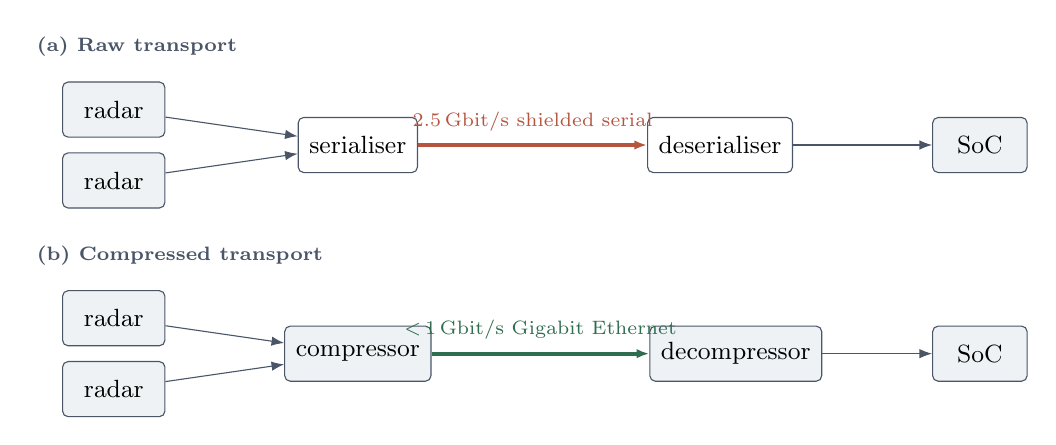
\begin{tikzpicture}[font=\small,
  box/.style={draw=slate,fill=white,rounded corners=2pt,minimum height=7mm,inner xsep=4pt},
  rad/.style={box,fill=lightbg,minimum width=13mm},
  lbl/.style={font=\scriptsize,text=slate}]

% ---- top: without compression
\node[lbl,anchor=west] at (-0.2,1.9) {\textbf{(a) Raw transport}};
\node[rad] (r1) at (0.9,1.1) {radar};
\node[rad] (r2) at (0.9,0.2) {radar};
\node[box,minimum width=14mm] (ser) at (4.0,0.65) {serialiser};
\node[box,minimum width=14mm] (des) at (8.6,0.65) {deserialiser};
\node[box,minimum width=12mm,fill=lightbg] (soc) at (11.9,0.65) {SoC};
\draw[-{Latex[length=1.6mm]},slate] (r1) -- (ser);
\draw[-{Latex[length=1.6mm]},slate] (r2) -- (ser);
\draw[-{Latex[length=1.6mm]},warm,line width=1.4pt] (ser) -- node[above,lbl,text=warm,yshift=1pt]{\SI{2.5}{Gbit/s} shielded serial} (des);
\draw[-{Latex[length=1.6mm]},slate] (des) -- (soc);

% ---- bottom: with compression
\node[lbl,anchor=west] at (-0.2,-0.75) {\textbf{(b) Compressed transport}};
\node[rad] (q1) at (0.9,-1.55) {radar};
\node[rad] (q2) at (0.9,-2.45) {radar};
\node[box,minimum width=16mm,fill=lightbg] (cmp) at (4.0,-2.0) {compressor};
\node[box,minimum width=18mm,fill=lightbg] (dec) at (8.8,-2.0) {decompressor};
\node[box,minimum width=12mm,fill=lightbg] (soc2) at (11.9,-2.0) {SoC};
\draw[-{Latex[length=1.6mm]},slate] (q1) -- (cmp);
\draw[-{Latex[length=1.6mm]},slate] (q2) -- (cmp);
\draw[-{Latex[length=1.6mm]},green2,line width=1.4pt] (cmp) -- node[above,lbl,text=green2,yshift=1pt]{$<$\,\SI{1}{Gbit/s} Gigabit Ethernet} (dec);
\draw[-{Latex[length=1.6mm]},slate] (dec) -- (soc2);
\end{tikzpicture}
\caption[Raw versus compressed radar transport]{The economic argument for
sensor-edge compression. Compressing by a factor of \num{2.5} or better at the
radar module replaces an expensive shielded high-speed serial link with
standard Gigabit Ethernet, without changing what the central processor
receives.}
\label{fig:arch}
\end{figure}

\section{Why the compressor must be lossless}
\label{sec:lossless}

It is tempting to relax the requirement. Lossy compression reaches much higher
ratios, and radar data is noisy anyway, so surely a little extra noise is
harmless?

It is not, and the reason is specific rather than philosophical. The
compressor sits \emph{upstream} of detection. Whatever it discards is
discarded before the detector ever sees it, and the detector's job is to find
weak returns close to the noise floor --- a pedestrian at range, a motorcycle
between two trucks. Lossy compression raises the noise floor precisely where
the margin is thinnest. Chapter~\ref{ch:results} quantifies this: Block
Adaptive Quantization, a respected lossy scheme, reaches a compression ratio
comparable to the lossless coders studied here but misses nearly three times as
many real detections and invents nearly nine times as many false ones.

Losslessness also has a practical virtue that matters enormously for a project
of this kind: it makes verification unambiguous. The pass criterion is that
every reconstructed sample equals its original exactly. There is no tolerance
to argue about, no distortion metric to trade off. A single differing bit
anywhere in \num{157} million samples is a defect, and the test reports it as
one. Section~\ref{sec:defects} describes two defects that were found exactly
this way and would have been invisible under any tolerance-based criterion.

\section{Objectives}
\label{sec:objectives}

The starting point for this thesis is the master's work of Lukas Kiem
\cite{kiem2025}, which evaluated a wide range of radar compression schemes and
identified Doppler Redundancy Hybrid Encoding as the best of them, reaching a
compression ratio of \num{3.2} at a latency of \SI{0.08}{\milli\second} on a
Zynq UltraScale+ device. Kiem's work left three openings, which became the
objectives of this thesis:

\begin{enumerate}
\item \textbf{Validate on real data.} Kiem's FPGA implementation was exercised
with synthetic stimulus. This thesis drives both compressors with real captured
data --- 50 consecutive frames from a Texas Instruments MMWCAS-RF-EVM cascade,
taken from the public ColoRadar dataset \cite{kramer2022} --- through the entire
verification chain, from MATLAB to RTL co-simulation.

\item \textbf{Broaden the algorithm comparison.} DRHE is compared here not only
against the schemes Kiem considered but against a second-order linear
predictive coder with Yule--Walker coefficients, and against a
\emph{no-prediction} baseline that turns out to be the most informative
comparison of all.

\item \textbf{Implement the complete pipeline.} Kiem implemented compression
only. This thesis implements compression \emph{and} decompression for both
algorithms, which is what makes bit-exact verification possible at every level,
and which exposed a subtle encoder/decoder divergence described in
Section~\ref{sec:defect32768}.
\end{enumerate}

\section{Contributions}
\label{sec:contributions}

The substantive contributions of this thesis are:

\begin{enumerate}
\item \textbf{A working, bit-exact, fully verified FPGA implementation of two
lossless radar compressors}, each with a matching decompressor, verified over
50 frames of real cascade radar data at three levels of abstraction (MATLAB
reference, HLS C-simulation, RTL co-simulation) with zero reconstruction error
at every level.

\item \textbf{The identification and correction of a prediction-axis error} in
applying slow-time predictive compression to time-division MIMO radar. Both
algorithms, applied the way the literature describes, performed \emph{worse
than no prediction at all}. Correcting the prediction lag to the transmitter
period recovers the intended gain, lifting measured compression from
\num{3.310} to \num{3.751} for DRHE and \num{3.385} to \num{3.697} for LPC.
This is, to the author's knowledge, not reported elsewhere.

\item \textbf{A decomposition of the compression ratio} into its three genuine
sources --- unused fixed-point container headroom, spectral sparsity, and
prediction --- which shows that the headline ratios reported in this field are
substantially a property of sensor gain staging rather than of the algorithm.

\item \textbf{Two implementation defects found and fixed}, both invisible on
real data and both caught by synthetic edge-case testing: an unrepresentable
residual value that aliased onto a different value, and a wide-integer to
floating-point conversion that silently returned zero.

\item \textbf{Three corrections to the surrounding literature and to the
author's own earlier reporting}: a throughput figure quoted in gibibits and
compared against decimal figures; a detection metric labelled as a false
positive rate that is in fact a false discovery rate; and two malformed source
citations.
\end{enumerate}

\section{How to read this report}
\label{sec:structure}

The report is written to be self-contained for a reader who knows some signal
processing and digital design but nothing in particular about radar or about
compression.

\textbf{Chapter~\ref{ch:background}} builds up the necessary background from
first principles: how an FMCW radar turns a frequency sweep into a range
measurement, what ``slow time'' and Doppler mean, how MIMO and time-division
multiplexing produce a virtual array, what is actually in the data that has to
be compressed, how lossless compression works in general, and what an FPGA
gives you and charges you for. A reader already fluent in these can skip to
Section~\ref{sec:sota}.

\textbf{Chapter~\ref{ch:algorithms}} specifies the two algorithms and the
entropy coder they share, in enough detail to reimplement them.

\textbf{Chapter~\ref{ch:method}} sets out the four-phase verification framework
and defines every metric used, including several that are commonly used
loosely.

\textbf{Chapter~\ref{ch:implementation}} describes the hardware architectures
and the two defects.

\textbf{Chapter~\ref{ch:results}} reports results, and is where the audit and
the prediction-axis correction appear.

\textbf{Chapter~\ref{ch:discussion}} discusses what the numbers support and what
they do not, and \textbf{Chapter~\ref{ch:conclusion}} concludes.

% ===================================================================
\chapter{Background}
\label{ch:background}

This chapter assumes no prior knowledge of radar. It builds up, in order, what
the radar measures, how it measures it, what the resulting data looks like, why
there is so much of it, how lossless compression works in general, and what an
FPGA can do about it. Each section ends with the specific fact that the later
chapters depend on.

\section{How an FMCW radar measures range}
\label{sec:fmcw}

\subsection{The chirp}

Automotive radar is almost universally \emph{frequency-modulated continuous
wave} (FMCW). Instead of emitting a short pulse and timing the echo --- which
would demand impractically fast electronics for the distances involved --- an
FMCW radar transmits continuously, sweeping its frequency linearly upward over
a short interval. One such sweep is called a \emph{chirp}. The sensor used here
sweeps \SI{1.798}{\giga\hertz} of bandwidth around a \SI{77}{\giga\hertz}
centre frequency in \SI{78.5}{\micro\second}.

When the chirp reflects off an object at range $R$, the echo arrives delayed by
the round-trip time
\begin{equation}
\tau = \frac{2R}{c},
\end{equation}
where $c$ is the speed of light. Because the transmitter has kept sweeping in
the meantime, the echo's frequency at any instant is lower than what is
currently being transmitted, by an amount proportional to the delay. If the
chirp sweeps $B$ hertz in $T_c$ seconds, the sweep slope is $S = B/T_c$ and the
frequency difference is
\begin{equation}
\label{eq:beat}
f_b = S\,\tau = \frac{2 S R}{c}.
\end{equation}

\begin{figure}[t]
\centering
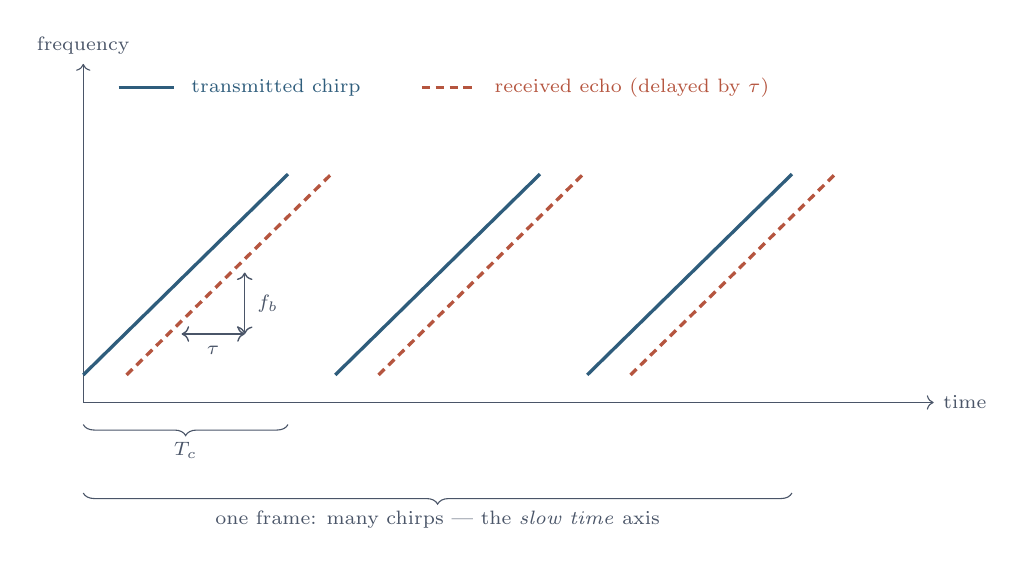
\begin{tikzpicture}[font=\small]
% axes
\draw[->,slate] (0,0) -- (10.8,0) node[right,font=\scriptsize]{time};
\draw[->,slate] (0,0) -- (0,4.3) node[above,font=\scriptsize]{frequency};
% legend (clear of the chirps)
\draw[accent,line width=1.2pt] (0.45,4.0) -- (1.15,4.0);
\node[font=\scriptsize,text=accent,anchor=west] at (1.25,4.0) {transmitted chirp};
\draw[warm,line width=1.2pt,densely dashed] (4.3,4.0) -- (5.0,4.0);
\node[font=\scriptsize,text=warm,anchor=west] at (5.1,4.0) {received echo (delayed by $\tau$)};
% transmitted chirps
\foreach \s in {0,3.2,6.4}{ \draw[accent,line width=1.2pt] (\s,0.35) -- (\s+2.6,2.9); }
% received (delayed)
\foreach \s in {0,3.2,6.4}{ \draw[warm,line width=1.2pt,densely dashed] (\s+0.55,0.35) -- (\s+3.15,2.9); }
% delay + beat annotation on first chirp
\draw[slate,dotted] (1.25,0.87) -- (2.05,0.87);
\draw[<->,slate,line width=0.5pt] (1.25,0.87) -- (2.05,0.87)
      node[midway,below,font=\scriptsize,text=slate,yshift=-1pt]{$\tau$};
\draw[<->,slate,line width=0.5pt] (2.05,0.87) -- (2.05,1.65)
      node[midway,right,font=\scriptsize,text=slate,xshift=1pt]{$f_b$};
% chirp duration brace
\draw[decorate,decoration={brace,amplitude=4pt,mirror},slate]
   (0,-0.28) -- (2.6,-0.28) node[midway,below,font=\scriptsize,text=slate,yshift=-3pt]{$T_c$};
\draw[decorate,decoration={brace,amplitude=4pt,mirror},slate]
   (0,-1.15) -- (9.0,-1.15) node[midway,below,font=\scriptsize,text=slate,yshift=-3pt]
   {one frame: many chirps --- the \emph{slow time} axis};
\end{tikzpicture}
\caption[FMCW chirp and beat frequency]{FMCW operation. Each chirp sweeps
linearly in frequency. The echo is a delayed copy, so at any instant the
transmitted and received frequencies differ by $f_b = S\tau$, proportional to
target range. A frame consists of many such chirps in succession; the axis
running across chirps is called \emph{slow time} and is where Doppler
information lives.}
\label{fig:chirp}
\end{figure}

A mixer multiplies the transmitted and received signals, producing a
low-frequency \emph{beat} or intermediate-frequency signal at exactly $f_b$.
That signal is low-pass filtered and digitised by an analog-to-digital
converter (ADC) at a modest rate --- \SI{8}{\mega\hertz} here, rather than the
tens of gigahertz the raw RF would need. This is the central trick of FMCW: it
converts a timing measurement that would need picosecond resolution into a
frequency measurement that an ordinary ADC can make.

\subsection{From beat frequency to a range profile}

Measuring $f_b$ is a spectral estimation problem, so the natural tool is the
Fourier transform. Taking an $N_s$-point FFT across the $N_s$ ADC samples of a
single chirp produces a \emph{range profile}: bin $n$ of the FFT corresponds,
through Equation~\eqref{eq:beat}, to range
\begin{equation}
R_n = n \cdot \frac{c}{2B},
\end{equation}
so the range resolution is
\begin{equation}
\Delta R = \frac{c}{2B} \approx \SI{8.3}{\centi\metre}
\end{equation}
for the \SI{1.798}{\giga\hertz} bandwidth used here. A peak in the range
profile is an object. This first transform is called the \textbf{Range FFT},
and its output is the data this thesis compresses.

\subsection{Slow time and Doppler}

A single chirp gives range but not velocity. To get velocity, the radar
transmits many chirps in rapid succession --- a \emph{frame} --- and looks at
how the \emph{phase} of a given range bin evolves from chirp to chirp.

The reasoning is worth spelling out, because the whole of DRHE rests on it. A
target at range $R$ produces a range-FFT value whose phase is
$\theta = -4\pi R/\lambda$, where $\lambda$ is the wavelength. Over the
chirp-to-chirp interval $T$, a target moving at radial velocity $v$ changes
range by $vT$, so its phase changes by
\begin{equation}
\label{eq:dopplerphase}
\Delta\theta = -\frac{4\pi v T}{\lambda}.
\end{equation}
At \SI{77}{\giga\hertz}, $\lambda \approx \SI{3.9}{\milli\metre}$, so even a
very slow target produces a measurable phase step --- which is exactly why
radar is good at velocity. Critically for compression, $\Delta\theta$ is
\emph{constant} for a target at constant velocity. The phase of a given range
bin therefore advances linearly across chirps, and its magnitude barely changes
at all. That is a highly predictable sequence, and predictable sequences
compress.

The axis running across chirps within a frame is called \textbf{slow time}, as
opposed to the \emph{fast time} axis of samples within a chirp. Taking a second
FFT along slow time resolves $\Delta\theta$ into velocity: this is the
\textbf{Doppler FFT}.

\begin{keybox}
\textbf{Carry forward:} slow time is where the redundancy is. A target at
constant velocity produces a range-bin sequence whose magnitude is nearly
constant and whose phase advances by a constant increment. Both DRHE and LPC
exist to exploit exactly this.
\end{keybox}

\section{Angle, MIMO and the virtual array}
\label{sec:mimo}

\subsection{Why more antennas}

Range and velocity are not enough to drive a car. The radar also has to know
\emph{where} a target is in angle, and how well it can separate two targets at
the same range and velocity but different bearings.

Angle is measured by comparing the phase of the same echo at physically
separated receive antennas. A wavefront arriving at angle $\phi$ reaches
adjacent antennas, spaced $d$ apart, with a path difference $d\sin\phi$, hence
a phase difference
\begin{equation}
\label{eq:steering}
\Delta\psi = \frac{2\pi d \sin\phi}{\lambda}.
\end{equation}
An FFT across the receive-antenna axis --- the \textbf{Angle FFT} --- turns
those phase differences into a bearing estimate. The angular resolution
improves with the physical size of the array, which in practice means with the
number of elements.

\subsection{MIMO: buying antennas cheaply}

Building a large physical receive array is expensive. Multiple-Input
Multiple-Output (MIMO) radar gets the same effect more cheaply. If $N_t$
transmitters and $N_r$ receivers are arranged suitably, and the signal from
each transmitter can be separated at each receiver, then each of the
$N_t \times N_r$ transmit--receive pairs behaves like an element of a
\emph{virtual array}. The sensor used here has $N_t = 12$ and $N_r = 16$,
giving \num{192} virtual elements from \num{28} physical antennas.

\subsection{Time-division multiplexing, and why it matters here}
\label{sec:tdm}

The separability requirement has to be met somehow. The simplest method, and
the one this sensor uses, is \emph{time-division multiplexing} (TDM): the
transmitters fire one at a time, in a fixed rotation, so whatever a receiver
hears during transmitter $t$'s slot must have come from transmitter $t$.

TDM is simple and robust, and it has one consequence that this thesis turns
out to hinge on. Inside every repetition of the frame --- every ``chirp loop''
--- all $N_t$ transmitters fire in sequence before the loop repeats. When the
resulting data is laid out as a two-dimensional array of (ramp, range bin),
which is how a streaming compressor sees it, the ramp index is
\begin{equation}
\label{eq:rampindex}
m = c\,N_t + t,
\qquad c \in [0, N_c), \quad t \in [0, N_t),
\end{equation}
where $c$ indexes the chirp loop and $t$ the transmitter. The transmitter index
varies \emph{fastest}.

This is the correct physical time order. It is also, as Figure~\ref{fig:tdm}
makes visual, a trap. Ramp $m$ and ramp $m-1$ are different physical
transmitters $N_t - 1$ times out of $N_t$. They are separated in \emph{space}
by the array baseline, not in \emph{time} by a pulse interval, and the phase
relationship between them is governed by Equation~\eqref{eq:steering} --- the
target's bearing --- not by Equation~\eqref{eq:dopplerphase} --- the target's
velocity. The genuine slow-time neighbour of ramp $m$, the one whose phase
differs by a Doppler step, is ramp $m - N_t$.

\begin{figure}[t]
\centering
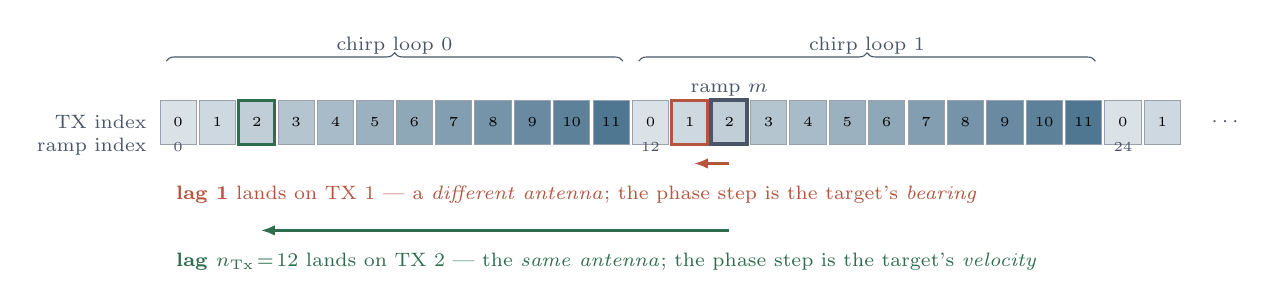
\begin{tikzpicture}[font=\small,x=0.50cm,y=0.50cm]
\foreach \i in {0,...,25}{
  \pgfmathtruncatemacro{\tx}{mod(\i,12)}
  \pgfmathsetmacro{\shade}{18+\tx*6}
  \node[draw=slate!55,line width=0.3pt,fill=accent!\shade,minimum width=0.46cm,
        minimum height=0.56cm,inner sep=0pt,font=\tiny] (c\i) at (\i,0) {\tx};
}
\node[anchor=east,font=\scriptsize,text=slate] at (-0.55,0) {TX index};
\node[anchor=west,font=\scriptsize,text=slate] at (26.0,0) {$\cdots$};
% highlight the three cells that matter
\node[draw=green2,line width=1.1pt,minimum width=0.46cm,minimum height=0.56cm,inner sep=0pt] at (2,0) {};
\node[draw=warm,line width=1.1pt,minimum width=0.46cm,minimum height=0.56cm,inner sep=0pt] at (13,0) {};
\node[draw=slate,line width=1.4pt,minimum width=0.46cm,minimum height=0.56cm,inner sep=0pt] at (14,0) {};
\node[font=\scriptsize,text=slate,anchor=south] at (14,0.40) {ramp $m$};
% ramp ruler
\foreach \i/\l in {0/0,12/12,24/24}{ \node[font=\tiny,text=slate] at (\i,-0.62) {\l}; }
\node[anchor=east,font=\scriptsize,text=slate] at (-0.55,-0.62) {ramp index};
% chirp loop braces
\draw[decorate,decoration={brace,amplitude=3pt},slate] (-0.3,1.55) -- (11.3,1.55)
   node[midway,above,font=\scriptsize,text=slate,yshift=-1pt]{chirp loop 0};
\draw[decorate,decoration={brace,amplitude=3pt},slate] (11.7,1.55) -- (23.3,1.55)
   node[midway,above,font=\scriptsize,text=slate,yshift=-1pt]{chirp loop 1};
% lag arrows, drawn under the strip
\draw[warm,line width=1.0pt,-{Latex[length=1.8mm]}] (14,-1.05) -- (13.1,-1.05);
\node[font=\scriptsize,text=warm,anchor=west] at (-0.3,-1.85)
   {\textbf{lag 1} lands on TX 1 --- a \emph{different antenna}; the phase step is the target's \emph{bearing}};
\draw[green2,line width=1.0pt,-{Latex[length=1.8mm]}] (14,-2.75) -- (2.1,-2.75);
\node[font=\scriptsize,text=green2,anchor=west] at (-0.3,-3.55)
   {\textbf{lag $n_{\mathrm{Tx}}\!=\!12$} lands on TX 2 --- the \emph{same antenna}; the phase step is the target's \emph{velocity}};
\end{tikzpicture}
\caption[TDM-MIMO ramp interleaving]{Why ``the previous ramp'' is the wrong
neighbour on a TDM-MIMO cascade. Each cell is one ramp, labelled with the
transmitter that produced it; the twelve transmitters rotate inside every chirp
loop. Predicting ramp $m$ from ramp $m-1$ (red) crosses a transmitter boundary
eleven times out of twelve, so the two ramps differ by the target's array
steering phase. Predicting from ramp $m - n_{\mathrm{Tx}}$ (green) stays on the
same physical antenna and therefore on the genuine Doppler axis.}
\label{fig:tdm}
\end{figure}

\begin{keybox}
\textbf{Carry forward:} on a TDM-MIMO radar the ramp axis is
transmitter-interleaved. Any algorithm that assumes consecutive ramps are
consecutive \emph{in time on the same antenna} --- which includes DRHE as
published, and a plain lag-1/lag-2 linear predictor --- is operating on the
wrong axis. This is the central finding of Chapter~\ref{ch:results}.
\end{keybox}

\section{The radar data cube, and why it is large}
\label{sec:cube}

Putting the three axes together gives the \emph{radar data cube}: fast time
(samples within a chirp) $\times$ slow time (ramps) $\times$ receive channel.
Three FFTs are applied along the three axes in turn, yielding range, velocity
and angle. Figure~\ref{fig:cube} shows the arrangement and where in the chain
this thesis intervenes.

\begin{figure}[t]
\centering
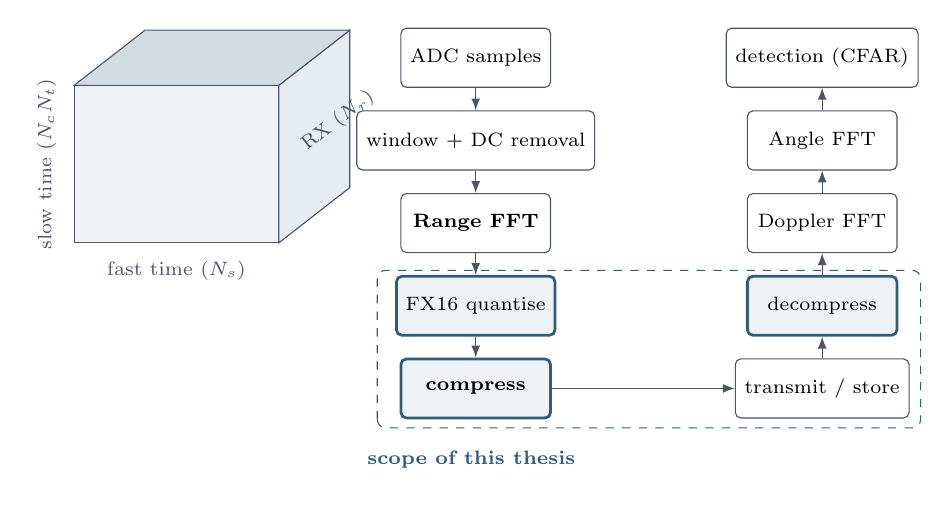
\begin{tikzpicture}[font=\small]
% cube
\begin{scope}[shift={(0,0)},scale=1.0]
  \draw[fill=lightbg,draw=slate] (0,0) -- (2.6,0) -- (2.6,2.0) -- (0,2.0) -- cycle;
  \draw[fill=accent!12,draw=slate] (2.6,0) -- (3.5,0.7) -- (3.5,2.7) -- (2.6,2.0) -- cycle;
  \draw[fill=accent!22,draw=slate] (0,2.0) -- (2.6,2.0) -- (3.5,2.7) -- (0.9,2.7) -- cycle;
  \node[font=\scriptsize,text=slate] at (1.3,-0.35) {fast time ($N_s$)};
  \node[font=\scriptsize,text=slate,rotate=90] at (-0.35,1.0) {slow time ($N_c N_t$)};
  \node[font=\scriptsize,text=slate,rotate=38] at (3.35,1.55) {RX ($N_r$)};
\end{scope}
% chain
\begin{scope}[shift={(5.1,0.25)},
  b/.style={draw=slate,fill=white,rounded corners=2pt,minimum width=19mm,minimum height=7.5mm,font=\scriptsize},
  h/.style={draw=accent,line width=1pt,fill=lightbg,rounded corners=2pt,minimum width=19mm,minimum height=7.5mm,font=\scriptsize}]
  \node[b] (a) at (0,2.1) {ADC samples};
  \node[b] (b) at (0,1.05) {window + DC removal};
  \node[b] (c) at (0,0.0) {\textbf{Range FFT}};
  \node[h] (d) at (0,-1.05) {FX16 quantise};
  \node[h] (e) at (0,-2.1) {\textbf{compress}};
  \node[b] (f) at (4.4,-2.1) {transmit / store};
  \node[h] (g) at (4.4,-1.05) {decompress};
  \node[b] (h2) at (4.4,0.0) {Doppler FFT};
  \node[b] (i) at (4.4,1.05) {Angle FFT};
  \node[b] (j) at (4.4,2.1) {detection (CFAR)};
  \foreach \x/\y in {a/b,b/c,c/d,d/e} {\draw[-{Latex[length=1.5mm]},slate] (\x) -- (\y);}
  \draw[-{Latex[length=1.5mm]},slate] (e) -- (f);
  \foreach \x/\y in {f/g,g/h2,h2/i,i/j} {\draw[-{Latex[length=1.5mm]},slate] (\x) -- (\y);}
  \node[font=\scriptsize,text=accent,align=left,anchor=west] at (-1.5,-3.0)
     {\textbf{scope of this thesis}};
  \draw[accent,dashed,rounded corners=3pt] (-1.25,-2.6) rectangle (5.65,-0.6);
\end{scope}
\end{tikzpicture}
\caption[Radar data cube and processing chain]{The radar data cube and the
processing chain. The compressor sits immediately after range-FFT and
fixed-point quantisation, before the data leaves the sensor. Everything
downstream --- Doppler FFT, angle FFT, detection --- sees the reconstructed
data, which for a lossless compressor is bit-identical to the original.}
\label{fig:cube}
\end{figure}

The volume follows directly. For the sensor used here, one frame is
\begin{equation}
N_s \times N_c \times N_r \times N_t
 = 256 \times 16 \times 16 \times 12 = \num{786432}
\end{equation}
complex samples. Each is two 16-bit integers, so a frame is
\SI{3145728}{\byte} --- exactly \SI{3}{\mebi\byte}. At a typical frame rate
this is gigabits per second from a single sensor, and a vehicle carries
several.

\section{Lossless compression: how it actually works}
\label{sec:compression}

\subsection{The two categories}

Compression divides into \emph{lossless}, where the decompressed data is
bit-identical to the input, and \emph{lossy}, where some information is
permanently discarded in exchange for a smaller payload \cite{sayood2017}.
Lossy compression can reach far higher ratios; lossless compression is bounded
by the information content of the data itself. Section~\ref{sec:lossless}
explained why this application needs the lossless kind.

\subsection{The bound: entropy}

There is a hard limit on lossless compression, and knowing it is what makes the
results in Chapter~\ref{ch:results} interpretable. If a source emits symbols
$x$ with probabilities $p(x)$, its \emph{order-0 entropy} is
\begin{equation}
\label{eq:entropy}
H = -\sum_x p(x) \log_2 p(x) \quad\text{bits per symbol},
\end{equation}
and no code that treats symbols independently can average fewer bits than $H$
\cite{sayood2017}. This gives a concrete yardstick: measure $H$ for the data,
compare it against what the coder actually achieves, and the gap is the coder's
inefficiency. Section~\ref{sec:decomposition} does exactly this, and finds the
entropy coder used here runs only \SI{6.2}{\percent} above the order-0 entropy
of its input --- which is good, and which means the room for improvement is not
in the entropy coder.

\subsection{The standard two-stage structure}

Almost every practical lossless compressor has the same shape
(Figure~\ref{fig:twostage}): a \emph{decorrelation} stage followed by an
\emph{entropy coding} stage.

\begin{figure}[t]
\centering
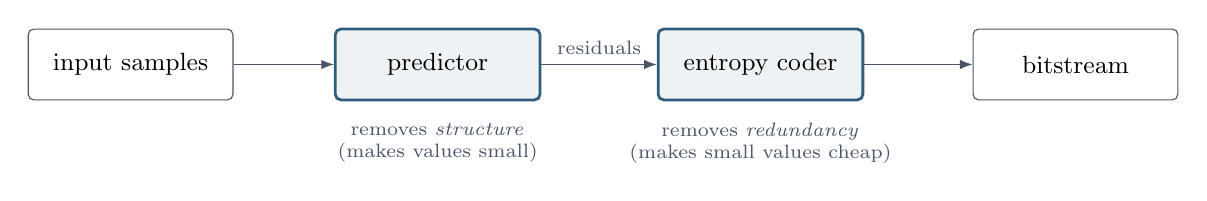
\begin{tikzpicture}[font=\small,
  b/.style={draw=slate,fill=white,rounded corners=2pt,minimum width=26mm,minimum height=9mm,font=\small},
  h/.style={draw=accent,line width=1pt,fill=lightbg,rounded corners=2pt,minimum width=26mm,minimum height=9mm,font=\small}]
\node[b] (in) at (0,0) {input samples};
\node[h] (p) at (3.9,0) {predictor};
\node[h] (e) at (8.0,0) {entropy coder};
\node[b] (out) at (12.0,0) {bitstream};
\draw[-{Latex[length=1.6mm]},slate] (in) -- (p);
\draw[-{Latex[length=1.6mm]},slate] (p) -- node[above,font=\scriptsize,text=slate]{residuals} (e);
\draw[-{Latex[length=1.6mm]},slate] (e) -- (out);
\node[font=\scriptsize,text=slate,align=center] at (3.9,-1.0)
  {removes \emph{structure}\\(makes values small)};
\node[font=\scriptsize,text=slate,align=center] at (8.0,-1.0)
  {removes \emph{redundancy}\\(makes small values cheap)};
\end{tikzpicture}
\caption[Two-stage lossless compressor]{The standard structure of a lossless
compressor. The two stages do different jobs and can fail independently ---
which is precisely what Chapter~\ref{ch:results} finds had happened.}
\label{fig:twostage}
\end{figure}

The \textbf{decorrelation} stage exploits structure. If consecutive samples are
similar, predict each one from its neighbours and transmit only the
\emph{residual}, the difference between prediction and truth. When the
prediction is good, residuals cluster tightly around zero even though the
original samples spanned the full dynamic range. Nothing is lost: given the
residual and the same prediction rule, the decoder reconstructs the original
exactly.

The \textbf{entropy coding} stage exploits the resulting skew in the
distribution. Values that occur often get short codewords; values that occur
rarely get long ones. Huffman coding \cite{huffman1952} is the classic
construction and produces the optimal prefix-free code for a known symbol
distribution.

Crucially, the two stages are independent. A predictor that fails --- that
produces residuals no more skewed than its input --- does not break the coder;
the coder simply carries on compressing whatever it is handed, and the
compression ratio can still look respectable. Detecting this requires
deliberately measuring what the coder achieves \emph{without} the predictor,
which is not a standard practice and which is how the central finding of this
thesis came to light.

\subsection{Open-loop versus closed-loop prediction}
\label{sec:closedloop}

One subtlety in predictive coding matters enough to state now, because it
caused a defect described in Section~\ref{sec:defect32768}.

The encoder predicts from past samples. So does the decoder --- but the decoder
does not have the past \emph{original} samples, only the past
\emph{reconstructed} ones. In \emph{open-loop} prediction the encoder uses the
originals; in \emph{closed-loop} prediction (classically, differential
pulse-code modulation, DPCM) the encoder reconstructs each sample exactly as
the decoder will, and predicts from that.

When compression is perfectly lossless the two are identical, because
reconstruction equals the original. The moment anything --- a saturation, a
rounding, a clamp --- makes reconstruction differ from the original by even one
bit, an open-loop encoder and its decoder begin predicting from different
histories and \emph{diverge}. With an IIR predictor, as in DRHE, that
divergence is then carried forward through every subsequent ramp. Closing the
loop confines the error to the affected sample.

\begin{keybox}
\textbf{Carry forward:} a compression ratio is the product of two independent
effects, and a healthy-looking ratio does not imply a working predictor. Always
measure the entropy coder alone as a baseline.
\end{keybox}

\section{The sensor and the dataset}
\label{sec:sensor}

\subsection{AWR2243 and the MMWCAS-RF-EVM}

The radar front end assumed throughout is the Texas Instruments AWR2243, a
76--\SI{81}{\giga\hertz} FMCW transceiver with three transmit and four receive
channels \cite{ti_awr2243}. Importantly for this work, the AWR2243 performs no
signal processing of its own: it transmits, receives, mixes and digitises, then
streams raw ADC samples out over a MIPI CSI-2 interface. It therefore exposes
exactly the payload that creates the transport bottleneck.

Four AWR2243 devices are cascaded on the MMWCAS-RF-EVM evaluation module,
giving \num{12} transmit and \num{16} receive channels on one synchronised
board --- the \num{192}-element virtual array of Section~\ref{sec:mimo}.

\subsection{ColoRadar}

Rather than synthetic stimulus, this thesis uses real captures from the public
ColoRadar dataset \cite{kramer2022}, which includes cascade recordings from
exactly this module across indoor, outdoor and subterranean environments.
Table~\ref{tab:capture} lists the relevant parameters. Fifty consecutive frames
were used throughout; that is \num{157286400} complex samples, or
\SI{150}{\mebi\byte} of raw data, which is enough to make a claim of
losslessness meaningful.

\begin{table}[t]
\centering
\caption{ColoRadar cascade capture parameters used throughout this thesis.}
\label{tab:capture}
\begin{tabular}{@{}llr@{}}
\toprule
Parameter & Symbol & Value \\
\midrule
ADC samples per chirp      & $N_s$ & 256 \\
Chirp loops per frame      & $N_c$ & 16 \\
Receive channels           & $N_r$ & 16 \\
Transmit channels (TDM)    & $N_t$ & 12 \\
Ramps per frame            & $N_c N_t$ & 192 \\
Fast-time sample rate      & $f_s$ & \SI{8}{\mega\hertz} \\
Chirp bandwidth            & $B$ & \SI{1.798}{\giga\hertz} \\
Chirp-to-chirp interval    & $T_c$ & \SI{78.5}{\micro\second} \\
Centre frequency           & $f_c$ & \SI{77}{\giga\hertz} \\
Range resolution           & $\Delta R$ & \SI{8.34}{\centi\metre} \\
Frame size (raw)           & --- & \SI{3145728}{\byte} \\
\bottomrule
\end{tabular}
\end{table}

Each complex sample is stored as two contiguous \texttt{int16} values. The
index of the sample at (fast-time $s$, chirp loop $c$, receiver $r$,
transmitter $t$) in the file is
\begin{equation}
i = 2\bigl(s + N_s(c + N_c(r + t N_r))\bigr),
\end{equation}
so the layout from slowest to fastest varying is $[t, r, c, s]$. Reshaping this
into the (fast time, ramp, receiver) cube the processing chain expects is what
produces the transmitter-interleaved ramp axis of Equation~\eqref{eq:rampindex}.

\section{Number representation and quantisation}
\label{sec:numbers}

\subsection{Fixed point versus floating point}

Hardware has to represent numbers somehow, and the choice is consequential.

\emph{Fixed-point} representation allocates a constant number of bits to the
integer and fractional parts, commonly written $Qm.n$. Because the binary point
never moves, addition, subtraction and multiplication are ordinary integer
operations: cheap, single-cycle, and small in silicon \cite{parhami2010}. The
price is a fixed dynamic range. Values too large wrap around; values too small
round to zero.

\emph{Floating-point} representation stores a sign, exponent and mantissa, so
the binary point moves with the magnitude \cite{ieee754}. This buys enormous
dynamic range but costs a great deal: every operation requires exponent
alignment, normalisation and special-case handling, which needs a dedicated
floating-point unit and takes multiple clock cycles. Chapter~\ref{ch:results}
shows this concretely --- the DRHE implementation's LUT count is dominated by
four floating-point transcendental functions per sample, and they are why it
misses its clock target.

\subsection{Quantisation error, and the FX16 step}
\label{sec:fx16}

The range-FFT output is naturally a complex floating-point quantity. Before it
can be compressed by a fixed-point pipeline it has to be quantised to 16-bit
integers --- the \textbf{FX16} step. This is a scaling followed by rounding:
\begin{equation}
\label{eq:scale}
\sigma = \frac{32767}{A_{\max}\,2^{\mathrm{shift}} \sum_k w_k \,/\, (2 N_s)},
\qquad
x_{\mathrm{FX16}} = \mathrm{round}(\sigma \cdot x),
\end{equation}
where $A_{\max}$ is the full-scale ADC amplitude and $w$ is the window applied
along fast time.

Two things about Equation~\eqref{eq:scale} matter later. First, the rounding
introduces an error bounded by half a least-significant bit, which acts as a
wideband noise floor \cite{widrow2008}; this is the dominant source of
detection degradation in the whole chain, and Chapter~\ref{ch:results}
separates it cleanly from the cost of compression. Second, and more
consequentially for this thesis, the scale factor is \emph{fixed} --- it is
calibrated from a theoretical full-scale ADC sinusoid, not from the data.
If the actual capture sits well below full scale, the top bits of every
resulting \texttt{int16} are structurally zero.
Section~\ref{sec:decomposition} shows that this is exactly what happens, and
that it accounts for more of the reported compression ratio than the
compression algorithms do.

\begin{keybox}
\textbf{Carry forward:} the FX16 scale factor is fixed and calibrated to
full scale. Whether the capture actually fills the container is a property of
the sensor's gain staging, and it silently inflates any compression ratio
measured downstream.
\end{keybox}

\section{FPGAs and high-level synthesis}
\label{sec:fpga}

\subsection{What an FPGA is}

A field-programmable gate array is a chip full of small configurable logic
blocks and configurable wiring between them. Rather than executing
instructions, an FPGA \emph{becomes} the circuit you describe. The practical
consequences for this application are three:

\begin{itemize}
\item \textbf{Parallelism.} A processor handles four receive channels one after
another. An FPGA can instantiate four copies of the datapath and do all four in
the same clock cycle. Every design in this thesis does exactly that.
\item \textbf{Deterministic latency.} There is no cache, no operating system,
no interrupt jitter. A design that takes \num{61253} cycles takes
\num{61253} cycles every time, which is what a safety-critical pipeline needs.
\item \textbf{Reconfigurability.} The design can be changed after fabrication,
which is what makes an FPGA the right platform for a thesis --- and what made
it practical to build, measure and then substantially revise two compressors
inside one project.
\end{itemize}

In production, a design proven on an FPGA is normally migrated into an ASIC or
into a fixed-function accelerator block inside a larger SoC, for cost and power
reasons \cite{kuon2008,nxp_an5375}. The FPGA here is a proof of concept, not a
proposed product.

\subsection{The four currencies: LUT, FF, BRAM, DSP}

FPGA resource usage is reported in four units, and it is worth knowing what
each is because the two algorithms in this thesis trade them against each other
in an interesting way.

\begin{description}[leftmargin=!,labelwidth=24mm,style=nextline,font=\normalfont\bfseries]
\item[LUT] \emph{Look-up table.} A small memory that implements an arbitrary
Boolean function of a few inputs. LUTs are the raw material of combinational
logic. Complicated arithmetic --- square roots, arctangents --- costs a lot of
LUTs.
\item[FF] \emph{Flip-flop.} A one-bit register. Flip-flops hold values between
clock cycles; deep pipelines need many of them.
\item[BRAM] \emph{Block RAM.} Dedicated on-chip memory, here counted in
\SI{18}{\kilo bit} units. Arrays that are too large to live in flip-flops go
here. BRAMs typically have two access ports, which becomes important below.
\item[DSP] \emph{DSP slice.} A hardened multiply--accumulate unit. Using a DSP
for a multiply is far cheaper than building one from LUTs.
\end{description}

The target device throughout is an AMD Kintex UltraScale+
\texttt{xcku5p-ffvb676-2-e}, which provides \num{216960} LUTs,
\num{433920} flip-flops, \num{960} \SI{18}{\kilo bit} BRAMs and \num{1824} DSP
slices.

\subsection{Pipelining, initiation interval and $F_{\max}$}
\label{sec:pipelining}

Three timing concepts recur throughout the results.

\textbf{Pipelining} splits a long computation into stages separated by
registers, so several inputs can be in flight at once. The \emph{depth} of a
pipeline is how many cycles a single input takes to traverse it.

\textbf{Initiation interval} (II) is how many cycles must elapse between
accepting one input and the next. $\mathrm{II} = 1$ means a new sample every
cycle, which is the goal. $\mathrm{II} = 2$ halves throughput. II is limited by
the tightest resource constraint in the loop body --- very often, as
Chapter~\ref{ch:results} shows, by the number of access ports on a block RAM.

\textbf{$F_{\max}$} is the highest clock frequency at which the longest
combinational path still settles within one period. A design that estimates
\SI{81.88}{\mega\hertz} cannot be clocked at \SI{100}{\mega\hertz} without
either redesign or a slower clock.

Latency, throughput and $F_{\max}$ interact: a frame of $K$ beats at
initiation interval $\mathrm{II}$ and clock $f$ takes roughly
$K \cdot \mathrm{II} / f$ seconds, \emph{plus} the pipeline depth once per
invocation. That last term is usually negligible --- and
Section~\ref{sec:tdmimpl} contains a case where it emphatically is not, costing
\num{65000} cycles that a naive model misses entirely.

\subsection{High-level synthesis}

Traditionally FPGA designs are written in a hardware description language such
as VHDL or Verilog, at the level of registers and wires. \emph{High-level
synthesis} (HLS) instead takes annotated C++ and generates the RTL
automatically. Loops become state machines; arrays become memories; pragmas
tell the tool to pipeline a loop, partition an array, or expose a port as an
AXI4-Stream interface.

HLS is used throughout this thesis for a specific reason beyond convenience:
because the design source is C++, the \emph{same source} can be compiled and
run as ordinary software against the MATLAB reference, before any hardware is
generated. That makes the verification ladder of Chapter~\ref{ch:method}
possible, and it is how both defects in Section~\ref{sec:defects} were caught
in seconds rather than in hours of RTL simulation.

\subsection{AXI4-Stream}

The interface used by both compressors is AXI4-Stream: a simple
valid/ready handshake carrying a fixed-width data word per beat. The designs
here accept \num{128} bits per beat --- four receive channels, each a 16-bit
real and a 16-bit imaginary part --- and emit \num{256} bits per beat of
compressed bitstream. A useful consequence for benchmarking is that
``\num{128} bits per cycle'' is the theoretical maximum input rate, and
therefore what a perfectly efficient design at $\mathrm{II}=1$ would achieve.
Section~\ref{sec:kiemcompare} uses this to resolve an ambiguity in a published
throughput figure.

\section{Related work and the baseline}
\label{sec:sota}

\subsection{Deterministic industrial schemes}

Because automotive safety systems demand bounded latency, commercial radar
processors use lightweight deterministic compressors. Texas Instruments uses
Exponential-Golomb Encoding \cite{ti_ege}; NXP's S32R family uses block
floating-point formats such as CP4D, in which several mantissas share one
exponent \cite{nxp_an5375}. These are described as ``near lossless'' --- CP4D
introduces under \SI{0.25}{\decibel} of signal loss --- and reach ratios of
roughly \num{2} to \num{4}.

\subsection{Block Adaptive Quantization}

BAQ originates in synthetic aperture radar \cite{kwok1989}. It divides the data
into blocks, estimates each block's statistics, and adapts the quantiser step
size accordingly, so weak blocks are quantised finely and strong blocks
coarsely. It is lossy. It appears in this thesis as a comparison point, and
Chapter~\ref{ch:results} shows what its losses cost in detection terms.

\subsection{Neural and spectral approaches}

Autoencoder-based compressors reach high ratios but are expensive to deploy at
the sensor \cite{cheng2021}. AdaRadar \cite{park2026} avoids this by keeping the
edge side simple --- a discrete cosine transform and spectral pruning --- and
placing the neural decoder at the SoC, with a feedback loop that adapts the
rate to downstream perception performance. These are outside the scope of this
thesis, which concerns itself with lossless schemes, but they define the upper
end of the ratio spectrum.

\subsection{The baseline: Kiem's thesis}
\label{sec:kiembaseline}

The direct predecessor of this work is Lukas Kiem's master's thesis
\cite{kiem2025}, which performed a design-space exploration across
Exponential-Golomb variants, Infineon common-exponent formats, and predictive
coders, and concluded that Doppler Redundancy Hybrid Encoding gave the best
combination of compression ratio, noise-floor impact and detection accuracy. He
implemented DRHE on a Zynq UltraScale+ device, reporting a compression ratio of
\num{3.2}, an IP-core latency of \SI{230}{\nano\second} and a throughput of
``\SI{11.92}{Gbit\per\second}'' at \SI{100}{\mega\hertz}.

That thesis is the source of the DRHE specification used here, including the
filter coefficients and the Huffman dictionary, both of which were verified
entry-by-entry against it (Section~\ref{sec:huffman}). It left three gaps ---
synthetic-only validation, a narrow algorithm comparison, and a
compression-only implementation --- which Section~\ref{sec:objectives} listed as
this thesis's objectives.

It also, as Chapter~\ref{ch:results} shows, contains an assumption that does not
survive the move to a TDM-MIMO cascade. That is not a criticism of the work: a
single-transmitter radar has no transmitter-interleaved ramp axis, and on such
a radar the specification is correct as written. It becomes wrong only when
applied, unmodified, to a sensor of a different kind --- which is exactly what
this thesis did before measuring it.

\section{Summary of what the later chapters assume}

\begin{enumerate}
\item The data to be compressed is the \emph{range-FFT output}, quantised to
16-bit integers, arranged as (ramp $\times$ range bin $\times$ receiver).
\item The redundancy worth exploiting lives along \emph{slow time}: a target at
constant velocity gives nearly constant magnitude and a constant phase
increment.
\item On this sensor the ramp axis is \emph{transmitter-interleaved}, so the
slow-time neighbour of ramp $m$ is ramp $m - N_t$, not ramp $m-1$.
\item A compression ratio is the product of a decorrelation gain and an
entropy-coding gain, and the two must be measured separately.
\item The FX16 scale factor is fixed to full scale, so container occupancy is a
confounding variable in any measured ratio.
\item FPGA cost is measured in LUTs, flip-flops, BRAMs and DSPs, and timing in
initiation interval, pipeline depth and $F_{\max}$.
\end{enumerate}

% ===================================================================
\chapter{The Two Algorithms}
\label{ch:algorithms}

Both compressors follow the two-stage structure of
Section~\ref{sec:compression}: a predictor that turns samples into small
residuals, followed by an entropy coder that turns small residuals into few
bits. They share the entropy coder exactly, which is deliberate --- it means
any difference in compression ratio between them is attributable entirely to
the predictor, and it is what makes the no-prediction baseline of
Chapter~\ref{ch:results} a fair comparison for both.

This chapter specifies the entropy coder first, then each predictor.

\section{The shared entropy coder: turning residuals into bits}
\label{sec:entropycoder}

This section is deliberately detailed. The entropy coder is where the
compression ratio is physically realised --- it is the only part of either
design that actually emits bits --- so understanding exactly what it charges
for is what makes the results of Chapter~\ref{ch:results} interpretable rather
than merely quotable.

\subsection{What a residual is}
\label{sec:whatresidual}

Let $x[m]$ be the sample to be transmitted and let $P$ be some rule --- the
\emph{predictor} --- that produces an estimate
\begin{equation}
\hat{x}[m] = P\bigl(x[m-1],\, x[m-2],\, \ldots\bigr)
\end{equation}
from samples that have \emph{already been transmitted}. The encoder does not
send $x[m]$. It sends the \emph{residual}
\begin{equation}
\label{eq:residualdef}
d[m] = x[m] - \hat{x}[m].
\end{equation}

The decoder, having already reconstructed $x[m-1], x[m-2], \ldots$, runs the
identical rule $P$ on them, obtains the identical $\hat{x}[m]$, and recovers
\begin{equation}
x[m] = d[m] + \hat{x}[m].
\end{equation}

Two things follow, and both matter.

\paragraph{Nothing is lost.}
Equation~\eqref{eq:residualdef} is a \emph{re-expression}, not an
approximation. Given $\hat{x}[m]$, the map $x \mapsto d$ is a bijection. The
sequence $\{d[m]\}$ carries exactly the information the sequence $\{x[m]\}$
carried --- no more, no less. This is why a predictive coder can be lossless at
all.

\paragraph{The predictor must be causal.}
$P$ may only use samples the decoder already has. This is not a stylistic
preference but a hard constraint: a predictor that peeked at $x[m]$ itself
would be unreproducible at the far end. It is also why
Section~\ref{sec:closedloop} makes such a point of \emph{which} version of the
past the encoder uses --- the originals or the reconstructions --- since those
differ the moment anything is not exactly lossless.

\subsection{Why a re-expression can be worth anything}

If no information is lost and none is gained, why is the residual sequence any
cheaper to write down?

Because the \emph{distribution} has changed, and a well-chosen code charges by
distribution. Table~\ref{tab:rawvsresid} shows this on real data: one range bin
of one receive channel, sixteen consecutive ramps, taken from frame~0 of the
ColoRadar capture.

\begin{table}[t]
\centering
\caption[Raw values against residuals]{The same sixteen real samples, written
two ways. Range bin 75, receive channel 1, ramps 168--183. Both rows carry
identical information.}
\label{tab:rawvsresid}
\small
\setlength{\tabcolsep}{3.4pt}
\begin{tabular}{@{}l*{16}{r}@{}}
\toprule
$m$ & 168 & 169 & 170 & 171 & 172 & 173 & 174 & 175 & 176 & 177 & 178 & 179 & 180 & 181 & 182 & 183\\
\midrule
$x$ (raw) & $-69$ & $-52$ & $59$ & $-6$ & $-29$ & $-15$ & $59$ & $-20$ & $-69$ & $-73$ & $-45$ & $84$ & $-73$ & $-50$ & $59$ & $-5$\\
$d$ (residual) & $3$ & $-3$ & $0$ & $-1$ & $1$ & $3$ & $-4$ & $3$ & $-1$ & $-2$ & $-1$ & $0$ & $-2$ & $4$ & $-1$ & $1$\\
\bottomrule
\end{tabular}
\end{table}

The raw values swing over $[-73, +84]$; writing any of them needs eight bits.
The residuals never leave $[-4, +4]$; four bits would do. Since the two rows
are informationally equivalent, that factor of two is free --- provided the
coder can be told about it.

And there is the catch. The bound $[-4,+4]$ holds for \emph{these} sixteen
samples. Somewhere else in the frame a target appears, or the scene changes,
and a residual of $400$ arrives. A fixed four-bit field cannot carry it. What
is needed is a code that spends few bits on the common case, many on the rare
one, and lets the decoder tell which is which.

\subsection{The parsing problem}

The naive approach fails immediately. Suppose the rule were ``small values get
four bits, large values get twelve''. When the decoder reads four bits, it has
no way to know whether it has just read a complete small value or the first
third of a large one. Variable-length coding is not merely a matter of writing
fewer bits; it is a matter of writing them so that the boundaries can be
recovered.

There are two standard answers:

\begin{enumerate}
\item \textbf{A prefix-free code over every possible value.} Assign every one
of the \num{65536} possible 16-bit residuals its own codeword, no codeword
being a prefix of another. This is optimal, and it is what a Huffman code over
the raw alphabet would give --- but it needs a \num{65536}-entry table, and the
table has to be derived from the data and transmitted alongside it.

\item \textbf{Split the value into a size and a payload.} Send a small
\emph{description of how big the value is}, coded with a prefix-free code over
a handful of symbols, followed by the value itself in exactly that many raw
bits. The decoder reads the size first, so it always knows how many bits to
read next.
\end{enumerate}

Both compressors here take the second route, which is the same construction
JPEG uses for DC coefficients. It is cheap in every respect that matters for
hardware: the prefix-free table has sixteen entries rather than \num{65536}, it
can be fixed at design time rather than derived per frame, and decoding a
symbol is a sixteen-way comparison rather than a tree walk.

\subsection{The category $S_4$}

The ``size'' half of the split is the category
\begin{equation}
\label{eq:s4}
S_4(v) =
\begin{cases}
0 & v = 0,\\[2pt]
\min\bigl(15,\ \lfloor \log_2 |v| \rfloor + 1\bigr) & v \neq 0,
\end{cases}
\end{equation}
which is simply the number of bits needed to write $|v|$. Its ranges are given
in Table~\ref{tab:catranges}.

\begin{table}[h]
\centering
\caption[S4 category ranges]{The first few categories. Category $k \geq 1$
covers $|v| \in [2^{k-1},\, 2^k - 1]$, which counting both signs is exactly
$2^k$ distinct values --- precisely what $k$ raw bits can enumerate.}
\label{tab:catranges}
\small
\begin{tabular}{@{}rlrl@{}}
\toprule
$S_4$ & values covered & count & \\
\midrule
0 & $v = 0$ & 1 & the only category with no payload\\
1 & $v \in \{-1, +1\}$ & 2 & \\
2 & $|v| \in \{2,3\}$ & 4 & \\
3 & $|v| \in [4,7]$ & 8 & \\
4 & $|v| \in [8,15]$ & 16 & \\
$\vdots$ & & & \\
15 & $|v| \in [16384, 32767]$ & \num{32768} & exactly fills 15 bits\\
\bottomrule
\end{tabular}
\end{table}

The design is tight by construction: category $k$ contains exactly $2^k$
values, so $k$ payload bits identify one of them with nothing wasted and
nothing left over. Section~\ref{sec:hole} shows what happens at the one place
where ``nothing left over'' turns out to be a problem.

\subsection{The APPEND bits}

The payload half is
\begin{equation}
\label{eq:append}
A(v) =
\begin{cases}
v & v \geq 0,\\
v + 2^{S_4(v)} - 1 & v < 0,
\end{cases}
\end{equation}
written in $S_4(v)$ raw bits.

The offset for negative values looks arbitrary but is doing something specific.
Table~\ref{tab:cat3} enumerates category~3 in full.

\begin{table}[h]
\centering
\caption[Category 3 enumerated]{Every codepoint of category 3. The negative
values map to patterns with a clear most significant bit, the positive values
to patterns with it set --- so the sign is recovered from that one bit without
transmitting a sign bit.}
\label{tab:cat3}
\small
\begin{tabular}{@{}rrlc@{}}
\toprule
$v$ & $A(v)$ & 3-bit pattern & MSB \\
\midrule
$-7$ & 0 & \texttt{000} & 0\\
$-6$ & 1 & \texttt{001} & 0\\
$-5$ & 2 & \texttt{010} & 0\\
$-4$ & 3 & \texttt{011} & 0\\
$+4$ & 4 & \texttt{100} & 1\\
$+5$ & 5 & \texttt{101} & 1\\
$+6$ & 6 & \texttt{110} & 1\\
$+7$ & 7 & \texttt{111} & 1\\
\bottomrule
\end{tabular}
\end{table}

Because positive values in category $k$ span $[2^{k-1}, 2^k - 1]$ --- exactly
the $k$-bit patterns with the top bit set --- and the offset maps the negatives
onto $[0, 2^{k-1} - 1]$ --- exactly those with it clear --- the sign falls out
of the payload for free. The decoder's rule is therefore
\begin{equation}
v = \begin{cases}
A & \text{if the MSB of the $S_4$ payload bits is set},\\
A - \bigl(2^{S_4} - 1\bigr) & \text{otherwise},
\end{cases}
\end{equation}
which in hardware is one bit test and one subtract.

\subsection{Cost, and the shape of the dictionary}
\label{sec:huffman}

The total cost of coding one residual is
\begin{equation}
\label{eq:cost}
L(v) = \underbrace{\ell\bigl(S_4(v)\bigr)}_{\text{Huffman codeword}}
     + \underbrace{S_4(v)}_{\text{payload}},
\end{equation}
where $\ell(\cdot)$ is the codeword length for that category. The dictionary is
\emph{fixed} --- not computed per frame --- which saves transmitting it and
removes a serial dependency from the hardware. Its lengths are
\begin{equation}
\ell = [\,4,3,2,2,2,5,6,7,8,9,10,11,14,14,13,12\,]\ \text{bits}.
\end{equation}
The full dictionary, codewords included, is in Appendix~\ref{app:huffman}.
Every one of the sixteen entries was verified against the published table
\cite[Table~A.1]{kiem2025}; all sixteen agree once the published
most-significant-bit-first codes are reversed for the least-significant-bit-first
packer used in this implementation.

Substituting into Equation~\eqref{eq:cost} gives the cost curve that governs
everything downstream:

\begin{table}[h]
\centering
\small
\begin{tabular}{@{}rrrrr@{}}
\toprule
$S_4$ & $|v|$ range & $\ell$ & payload & \textbf{total} \\
\midrule
0 & $0$        & 4 & 0 & \textbf{4}\\
1 & $1$        & 3 & 1 & \textbf{4}\\
2 & $2$--$3$   & 2 & 2 & \textbf{4}\\
3 & $4$--$7$   & 2 & 3 & \textbf{5}\\
4 & $8$--$15$  & 2 & 4 & \textbf{6}\\
5 & $16$--$31$ & 5 & 5 & \textbf{10}\\
6 & $32$--$63$ & 6 & 6 & \textbf{12}\\
7 & $64$--$127$& 7 & 7 & \textbf{14}\\
8 & $128$--$255$& 8 & 8 & \textbf{16}\\
\bottomrule
\end{tabular}
\end{table}

Three features of this curve deserve attention.

\paragraph{Everything below 16 is nearly free.}
A residual anywhere in $[-15, +15]$ costs between four and six bits. Against
sixteen raw bits that is already a compression ratio between \num{2.7} and
\num{4.0}, achieved without the predictor doing anything clever --- it only has
to keep residuals small.

\paragraph{There is a cliff at category 5.}
Cost jumps from six bits to ten. A residual of \num{15} costs six bits; a
residual of \num{16} costs ten. The coder is, by design, forgiving of small
errors and severe about larger ones.

\paragraph{Above category 8 the code loses.}
A residual of \num{128} costs sixteen bits --- exactly what the raw value
would have cost. Beyond that the coder actively expands. This is not a flaw:
it is the inevitable consequence of assigning short codewords to some symbols,
and it is why the \texttt{random-int16} edge case of
Section~\ref{sec:edgecases} expands the data by \SI{67}{\percent}.

The dictionary's shape encodes an assumption about the data --- that categories
2, 3 and 4 dominate, since those get the two-bit codewords.
Section~\ref{sec:bitbudget} measures whether that assumption holds.

\subsection{Worked example 1: one value, in full}

Take $v = -5$.

\begin{enumerate}
\item $|v| = 5$, and $\lfloor \log_2 5 \rfloor + 1 = 3$, so $S_4 = 3$.
\item $v < 0$, so $A(v) = -5 + 2^3 - 1 = 2$, written in three bits as
\texttt{010}.
\item The dictionary gives category 3 the codeword \texttt{00}, two bits.
\item The emitted bits are \texttt{00}\,\texttt{010} --- five bits, against
sixteen for the raw value.
\end{enumerate}

Decoding runs the same steps backwards. The decoder matches \texttt{00} against
the dictionary, recovers $S_4 = 3$, reads the next three bits \texttt{010},
sees the most significant is \texttt{0} so the value was negative, and computes
$2 - (2^3 - 1) = -5$.

\subsection{Worked example 2: sixteen real samples, both ways}
\label{sec:workedbig}

The single-value example shows the mechanism. The following example shows why
it matters, and it doubles as a concrete demonstration of the central result of
this thesis.

Table~\ref{tab:worked16} traces sixteen consecutive ramps of one range bin ---
the same bin as Table~\ref{tab:rawvsresid} --- through the DRHE predictor twice.
The left half predicts from ramp $m-1$, which is how the algorithm is described
in the literature. The right half predicts from ramp $m - n_{\mathrm{Tx}}$,
which Section~\ref{sec:tdm} argued is the true slow-time neighbour. Everything
else --- the filters, the coefficients, the entropy coder, the dictionary --- is
identical between the two halves. Only the lag differs.

\begin{table}[htbp]
\centering
\caption[Sixteen samples traced through both predictors]{Sixteen real samples
traced through DRHE at two prediction lags. Range bin 75, receive channel 1,
frame 0, ramps 168--183; real part shown, the imaginary part behaves
identically. The window is late enough in the frame that both predictors'
filters are fully converged. The two halves differ only in which earlier ramp
the prediction comes from.}
\label{tab:worked16}
\small
\setlength{\tabcolsep}{4pt}
\begin{tabular}{@{}rr r@{\hskip 10pt} rrrr @{\hskip 10pt} rrrr@{}}
\toprule
& & & \multicolumn{4}{c}{\textbf{predicted from ramp $m-1$}}
    & \multicolumn{4}{c}{\textbf{predicted from ramp $m-n_{\mathrm{Tx}}$}}\\
\cmidrule(lr){4-7}\cmidrule(lr){8-11}
$m$ & TX & $x$ & $\hat{x}$ & $d$ & $S_4$ & bits & $\hat{x}$ & $d$ & $S_4$ & bits\\
\midrule
168 & 0  & $-69$ & $67$  & $-136$ & 8 & 16 & $-72$ & $3$  & 2 & 4\\
169 & 1  & $-52$ & $-75$ & $23$   & 5 & 10 & $-49$ & $-3$ & 2 & 4\\
170 & 2  & $59$  & $81$  & $-22$  & 5 & 10 & $59$  & $0$  & 0 & 4\\
171 & 3  & $-6$  & $64$  & $-70$  & 7 & 14 & $-5$  & $-1$ & 1 & 4\\
172 & 4  & $-29$ & $24$  & $-53$  & 6 & 12 & $-30$ & $1$  & 1 & 4\\
173 & 5  & $-15$ & $-29$ & $14$   & 4 & 6  & $-18$ & $3$  & 2 & 4\\
174 & 6  & $59$  & $-6$  & $65$   & 7 & 14 & $63$  & $-4$ & 3 & 5\\
175 & 7  & $-20$ & $-83$ & $63$   & 6 & 12 & $-23$ & $3$  & 2 & 4\\
176 & 8  & $-69$ & $-93$ & $24$   & 5 & 10 & $-68$ & $-1$ & 1 & 4\\
177 & 9  & $-73$ & $-65$ & $-8$   & 4 & 6  & $-71$ & $-2$ & 2 & 4\\
178 & 10 & $-45$ & $-44$ & $-1$   & 1 & 4  & $-44$ & $-1$ & 1 & 4\\
179 & 11 & $84$  & $28$  & $56$   & 6 & 12 & $84$  & $0$  & 0 & 4\\
180 & 0  & $-73$ & $70$  & $-143$ & 8 & 16 & $-71$ & $-2$ & 2 & 4\\
181 & 1  & $-50$ & $-75$ & $25$   & 5 & 10 & $-54$ & $4$  & 3 & 5\\
182 & 2  & $59$  & $81$  & $-22$  & 5 & 10 & $60$  & $-1$ & 1 & 4\\
183 & 3  & $-5$  & $67$  & $-72$  & 7 & 14 & $-6$  & $1$  & 1 & 4\\
\midrule
\multicolumn{6}{r}{\textbf{total bits}} & \textbf{176} & & & & \textbf{66}\\
\multicolumn{6}{r}{bits per value} & 11.00 & & & & 4.12\\
\multicolumn{6}{r}{compression ratio} & 1.455 & & & & \textbf{3.879}\\
\bottomrule
\end{tabular}
\end{table}

The left half is a predictor that is barely working. Its residuals ($-136$,
$+23$, $-22$, $-70$, \ldots) are frequently \emph{larger in magnitude than the
samples they replace}, they land in categories 5 through 8, and they cost
\num{11.00} bits per value --- a compression ratio of \num{1.455}, which is to
say the entropy coder is salvaging a little from a predictor that has actively
made things worse.

The right half is the same predictor on the correct axis. Its residuals never
exceed 4 in magnitude, they land in categories 0 through 3, and they cost
\num{4.12} bits per value.

\begin{figure}[t]
\centering
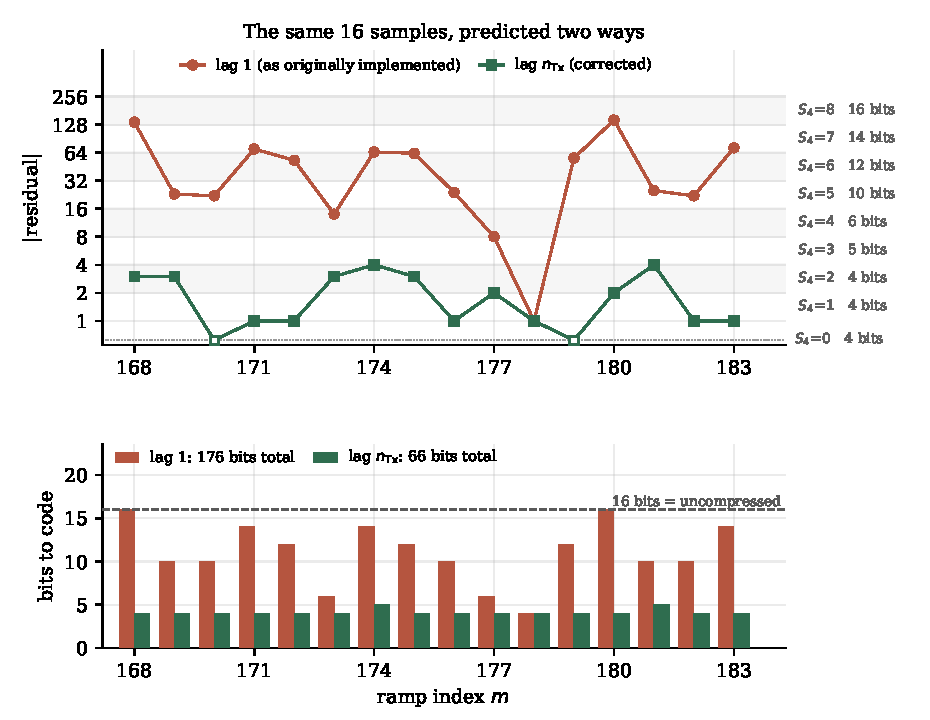
\includegraphics[width=\textwidth]{fig_worked.pdf}
\caption[The sixteen samples, plotted]{Table~\ref{tab:worked16} drawn. Above:
residual magnitude on a logarithmic scale, with the $S_4$ category bands and
their bit costs marked on the right; hollow markers are residuals of exactly
zero. Below: the bits each sample costs, against the \num{16} bits it would
have taken uncompressed. The lag-1 predictor spends \num{176} bits on this
window; the same predictor on the correct axis spends \num{66}.}
\label{fig:worked}
\end{figure}

\subsubsection*{Why the difference is so large}

Table~\ref{tab:workedpolar} answers this directly, and it is worth studying
because it is the mechanism behind every result in Chapter~\ref{ch:results}.
Recall from Section~\ref{sec:fmcw} that DRHE predicts magnitude with a smoother
and phase with a double integrator, both of which work when the quantity being
predicted changes slowly and smoothly.

\begin{table}[t]
\centering
\caption[Why the two lags differ]{The same window in polar coordinates. Against
ramp $m-1$ the magnitude moves by up to \num{22} and the phase jumps
unpredictably over the full $\pm\pi$ range. Against ramp $m-n_{\mathrm{Tx}}$ the
magnitude moves by at most \num{4} and the phase increment is essentially zero
--- a stationary target, exactly what the double integrator is built for.}
\label{tab:workedpolar}
\small
\setlength{\tabcolsep}{6pt}
\begin{tabular}{@{}rr rr @{\hskip 12pt} rr @{\hskip 12pt} rr@{}}
\toprule
& & \multicolumn{2}{c}{sample}
  & \multicolumn{2}{c}{change vs.\ $m-1$}
  & \multicolumn{2}{c}{change vs.\ $m-n_{\mathrm{Tx}}$}\\
\cmidrule(lr){3-4}\cmidrule(lr){5-6}\cmidrule(lr){7-8}
$m$ & TX & $|x|$ & $\angle x$ & $\Delta|x|$ & $\Delta\theta$ & $\Delta|x|$ & $\Delta\theta$\\
\midrule
168 & 0  & 74.1  & $-2.769$ & $-21.8$ & $-2.244$ & $-3.2$ & $\phantom{-}0.002$\\
169 & 1  & 91.3  & $-2.177$ & $17.2$  & $0.592$  & $-0.0$ & $-0.040$\\
170 & 2  & 101.0 & $-0.947$ & $9.8$   & $1.230$  & $-2.5$ & $\phantom{-}0.017$\\
171 & 3  & 110.2 & $-1.625$ & $9.1$   & $-0.678$ & $3.0$  & $-0.008$\\
172 & 4  & 107.0 & $-1.845$ & $-3.2$  & $-0.220$ & $-2.2$ & $\phantom{-}0.004$\\
173 & 5  & 112.0 & $-1.705$ & $5.0$   & $0.140$  & $-0.3$ & $\phantom{-}0.018$\\
174 & 6  & 97.0  & $0.917$  & $-15.0$ & $2.622$  & $-0.4$ & $\phantom{-}0.023$\\
175 & 7  & 81.5  & $1.819$  & $-15.5$ & $0.902$  & $0.4$  & $-0.027$\\
176 & 8  & 73.4  & $2.794$  & $-8.1$  & $0.975$  & $-0.1$ & $\phantom{-}0.043$\\
177 & 9  & 75.0  & $-2.913$ & $1.6$   & $0.576$  & $2.4$  & $\phantom{-}0.021$\\
178 & 10 & 95.3  & $-2.063$ & $20.3$  & $0.850$  & $0.9$  & $\phantom{-}0.005$\\
179 & 11 & 97.8  & $-0.537$ & $2.5$   & $1.526$  & $1.9$  & $-0.013$\\
180 & 0  & 77.5  & $-2.799$ & $-20.3$ & $-2.263$ & $3.4$  & $-0.031$\\
181 & 1  & 92.6  & $-2.141$ & $15.2$  & $0.659$  & $1.4$  & $\phantom{-}0.036$\\
182 & 2  & 102.6 & $-0.958$ & $10.0$  & $1.182$  & $1.6$  & $-0.011$\\
183 & 3  & 106.1 & $-1.618$ & $3.5$   & $-0.659$ & $-4.0$ & $\phantom{-}0.007$\\
\bottomrule
\end{tabular}
\end{table}

Look at the $\Delta\theta$ columns. Against ramp $m-1$ the phase increment is
$-2.244$, then $+0.592$, then $+1.230$, then $-0.678$ --- it swings over most
of $[-\pi, \pi]$ with no pattern a two-tap filter could follow. Against ramp
$m - n_{\mathrm{Tx}}$ it is $0.002$, $-0.040$, $0.017$, $-0.008$: essentially
zero, frame after frame, because this is a stationary target and twelve ramps
later the same antenna sees the same phase.

The magnitude column tells the same story: $\pm 22$ against the immediate
predecessor, $\pm 4$ against the same-transmitter predecessor.

The reason is the one given in Section~\ref{sec:tdm}. Ramps 168 and 167 were
transmitted by \emph{different antennas}, so the phase between them is set by
where the target is in \emph{angle}, via
Equation~\eqref{eq:steering} --- and the twelve transmitters are at twelve
different positions, so that phase jumps around on a period-12 pattern. Ramps
168 and 156 were transmitted by the \emph{same} antenna, so the phase between
them is set by how fast the target is \emph{moving}, via
Equation~\eqref{eq:dopplerphase} --- and it is not moving.

\subsubsection*{The actual bits}

It is worth seeing the bitstream itself. Coding the first six residuals of the
corrected column, using Equations~\eqref{eq:s4} and~\eqref{eq:append} and the
dictionary of Appendix~\ref{app:huffman}:

\begin{center}
\small
\begin{tabular}{@{}rrrlll r@{}}
\toprule
$d$ & $S_4$ & $A(d)$ & codeword & payload & emitted & bits\\
\midrule
$+3$ & 2 & 3 & \texttt{10}   & \texttt{11}  & \texttt{10\,11}   & 4\\
$-3$ & 2 & 0 & \texttt{10}   & \texttt{00}  & \texttt{10\,00}   & 4\\
$0$  & 0 & --- & \texttt{0101} & ---        & \texttt{0101}     & 4\\
$-1$ & 1 & 0 & \texttt{001}  & \texttt{0}   & \texttt{001\,0}   & 4\\
$+1$ & 1 & 1 & \texttt{001}  & \texttt{1}   & \texttt{001\,1}   & 4\\
$+3$ & 2 & 3 & \texttt{10}   & \texttt{11}  & \texttt{10\,11}   & 4\\
\bottomrule
\end{tabular}
\end{center}

\noindent
which concatenates to the 24-bit stream
\begin{center}
\texttt{1011\,1000\,0101\,0010\,0011\,1011}
\end{center}
carrying six samples that would have occupied \num{96} bits raw.

The same six samples on the uncorrected axis --- residuals $-136$, $+23$,
$-22$, $-70$, $-53$, $+14$ --- fall into categories 8, 5, 5, 7, 6 and 4 and
occupy $16 + 10 + 10 + 14 + 12 + 6 = \num{68}$ bits. Nearly three times as many,
for identical information.

\subsection{Decoding the same stream}

Decoding is the mirror image, and seeing it done confirms that no side
information beyond the fixed dictionary is needed. The decoder holds a bit
buffer and consumes from the low end.

\begin{enumerate}
\item Buffer is \texttt{1011\,1000\ldots}. Match the low bits against the
dictionary. The two-bit prefix \texttt{10} is category 2's codeword; no shorter
or longer entry can also match, because the reversed code set is prefix-free.
Consume two bits.
\item Category 2 means two payload bits. Read \texttt{11}, so $A = 3$. The most
significant of those two bits is set, so the value is positive: $d = +3$.
Consume two bits.
\item Add the prediction: the decoder has already reconstructed ramp
$168 - 12 = 156$ for this bin, runs the identical filters on it, obtains
$\hat{x} = -72$, and outputs $x = 3 + (-72) = -69$ --- which is the value in
Table~\ref{tab:worked16}.
\item Buffer is now \texttt{1000\,0101\ldots}. Match \texttt{10} again:
category 2. Read payload \texttt{00}, so $A = 0$, MSB clear, so
$d = 0 - (2^2 - 1) = -3$. Prediction $-49$, output $-52$. Correct.
\item Buffer is \texttt{0101\,0010\ldots}. Now \texttt{10} does \emph{not}
match, because the low two bits are \texttt{01}, which is no entry's codeword.
The four-bit prefix \texttt{0101} is category 0's codeword. Category 0 has no
payload and means $d = 0$ exactly. Prediction $59$, output $59$. Correct.
\end{enumerate}

Step 5 is the one that shows why prefix-freeness is doing real work: the
decoder never had to be told how long the next codeword would be.

\subsection{Where the bits actually go}
\label{sec:bitbudget}

The sixteen-sample window is illustrative but small. Table~\ref{tab:bitbudget}
gives the same accounting over an entire frame --- \num{196608} values, all
four receive channels --- which is what the compression ratio actually
integrates.

\begin{table}[t]
\centering
\caption[Bit budget by category]{Where the bits go, one frame, four receive
channels, \num{196608} values. ``\% values'' is how often a category occurs;
``\% bits'' is how much of the output it accounts for. The two columns are very
different, and the difference is the whole point of entropy coding.}
\label{tab:bitbudget}
\small
\setlength{\tabcolsep}{5pt}
\begin{tabular}{@{}rr rr @{\hskip 10pt} rr @{\hskip 10pt} rr@{}}
\toprule
& & \multicolumn{2}{c}{\textbf{no prediction}}
  & \multicolumn{2}{c}{\textbf{DRHE, lag 1}}
  & \multicolumn{2}{c}{\textbf{DRHE, lag $n_{\mathrm{Tx}}$}}\\
\cmidrule(lr){3-4}\cmidrule(lr){5-6}\cmidrule(lr){7-8}
$S_4$ & cost & \% values & \% bits & \% values & \% bits & \% values & \% bits\\
\midrule
0  & 4  & 16.71 & 14.61 & 11.78 & 9.81  & \textbf{18.85} & 17.87\\
1  & 4  & 28.57 & 24.97 & 22.01 & 18.33 & \textbf{32.94} & 31.22\\
2  & 4  & 31.45 & 27.49 & 31.95 & 26.60 & \textbf{34.40} & 32.60\\
3  & 5  & 14.66 & 16.02 & 22.21 & 23.12 & 11.31 & 13.40\\
4  & 6  & 4.31  & 5.65  & 6.46  & 8.07  & 1.49  & 2.12\\
5  & 10 & 1.75  & 3.82  & 2.36  & 4.92  & 0.50  & 1.18\\
6  & 12 & 1.15  & 3.01  & 1.43  & 3.58  & 0.29  & 0.82\\
7  & 14 & 1.14  & 3.47  & 1.09  & 3.17  & 0.18  & 0.59\\
8  & 16 & 0.19  & 0.66  & 0.65  & 2.17  & 0.03  & 0.13\\
9  & 18 & 0.07  & 0.29  & 0.06  & 0.23  & 0.01  & 0.05\\
\midrule
\multicolumn{2}{@{}l}{bits/value} & \multicolumn{2}{c}{4.576}
  & \multicolumn{2}{c}{4.803} & \multicolumn{2}{c}{\textbf{4.220}}\\
\multicolumn{2}{@{}l}{compression ratio} & \multicolumn{2}{c}{3.497}
  & \multicolumn{2}{c}{3.331} & \multicolumn{2}{c}{\textbf{3.792}}\\
\bottomrule
\end{tabular}
\end{table}

\begin{figure}[t]
\centering
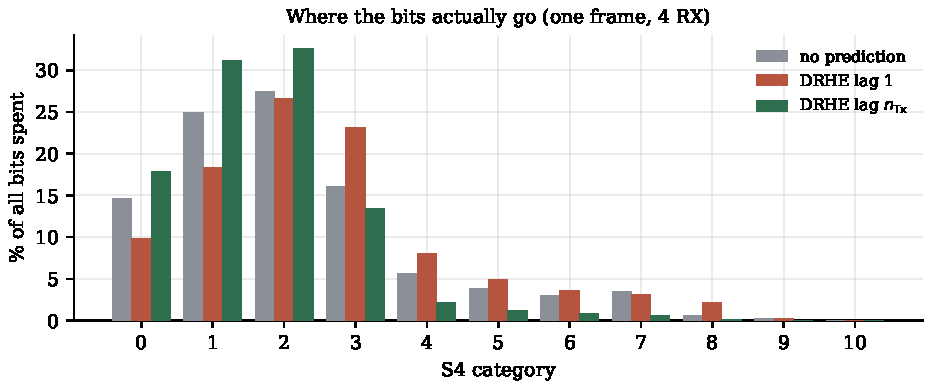
\includegraphics[width=\textwidth]{fig_bitbudget.pdf}
\caption[Bit budget by category]{The ``\% bits'' columns of
Table~\ref{tab:bitbudget} drawn. The corrected predictor concentrates spending
into the three four-bit categories; the lag-1 predictor pushes it out into
categories 3 through 8, where each value costs two to four times as much.}
\label{fig:bitbudget}
\end{figure}

Several things are visible here that the headline ratios hide.

\paragraph{The expensive categories are rare but not negligible.}
Under lag-1 prediction, categories 5 through 8 account for only
\SI{5.53}{\percent} of values but \SI{13.84}{\percent} of bits. One value in
eighteen is consuming one bit in seven. That asymmetry is exactly why the tail
of the residual distribution matters so much, and why
Figure~\ref{fig:residmag} plots the 99th percentile rather than the mean.

\paragraph{The correction works by emptying the tail.}
Comparing the last two column pairs: the corrected predictor moves
\SI{86.19}{\percent} of values into categories 0--2, all of which cost four
bits, and cuts categories 5--8 from \SI{5.53}{\percent} to
\SI{1.00}{\percent} of values. It is not that individual residuals got a little
smaller; it is that the expensive ones almost stopped occurring.

\paragraph{The lag-1 predictor loses to doing nothing in a specific way.}
Against the no-prediction column it \emph{gains} slightly in categories 0--2
but loses heavily in 3, 4 and 8. It is redistributing values upward, not
downward. A predictor that helps should hollow out the right-hand side of this
table; this one fills it in.

\subsection{How good is the coder itself?}

It is worth separating the coder's performance from the predictor's, since the
two are independent and only one of them turned out to be the problem.

The order-0 entropy of the raw FX16 values --- the theoretical floor for any
code that treats values independently, from Equation~\eqref{eq:entropy} --- is
\SI{4.094}{bits}. The coder achieves \SI{4.576}{bits} on the same data. That is
an overhead of \SI{0.48}{bits}, or \SI{11.8}{\percent}, for a dictionary fixed
at design time against a different dataset; on the five-frame average used in
Chapter~\ref{ch:results} the figure is \SI{6.2}{\percent}.

That is a good result, and it has a clear implication: \textbf{there is very
little left to win in the entropy coder}. Even a perfect, data-derived,
per-frame-optimal code would improve the compression ratio by only a few
per cent. All the remaining leverage is in the predictor --- which is what makes
a predictor that was contributing nothing such an expensive thing not to have
noticed.

One caveat is worth recording for future work. The dictionary gives its
two-bit codewords to categories 2, 3 and 4, which suits a distribution centred
there. After the prediction-axis correction the distribution has moved
\emph{down}: categories 0, 1 and 2 now hold \SI{86}{\percent} of values, and
category 0 --- exactly zero --- is paying four bits for what is now the second
most common symbol. Re-deriving the dictionary for the corrected residual
distribution is an obvious and cheap improvement that this thesis does not
make.

\subsection{A representability hole}
\label{sec:hole}

There is one value the code cannot represent, and it caused a real defect.

Category 15 spans $|v| \in [16384, 32767]$. Counting both signs that is exactly
$2^{15} = \num{32768}$ values, which exactly fills the fifteen payload bits ---
the tightness that Table~\ref{tab:catranges} noted as a virtue leaves no spare
codepoint. But \texttt{int16} arithmetic can produce $v = -32768$. Applying
Equation~\eqref{eq:append} gives
\begin{equation}
A(-32768) = -32768 + 32767 = -1,
\end{equation}
which truncated to fifteen bits is \texttt{0x7FFF} --- bit-for-bit the same
payload as $v = +32767$, with the same category and therefore the same
codeword. The two are indistinguishable on the wire, and the decoder returns
$+32767$.

This is not hypothetical. Section~\ref{sec:defect32768} reports it firing in a
synthetic edge case with a reconstruction error of \num{65535}, which is
precisely the distance from $-32768$ to $+32767$ --- a diagnostic number that
pointed straight back to this paragraph.

\section{DRHE: Doppler Redundancy Hybrid Encoding}
\label{sec:drhe}

\subsection{Why predict in polar coordinates}

Section~\ref{sec:fmcw} established what a range-bin sequence looks like across
slow time for a target at constant velocity: the \emph{magnitude} is nearly
constant, and the \emph{phase} advances by a constant increment. In Cartesian
$(I,Q)$ coordinates that is a point rotating on a circle --- both components
oscillate, and a simple difference between consecutive samples is large. In
polar coordinates the same sequence is two nearly-trivial signals: a constant
and a ramp.

DRHE therefore converts to polar, predicts magnitude and phase separately with
filters matched to those two shapes, converts the prediction back to Cartesian,
and subtracts.

\subsection{The two predictors}

For ramp $m$ and range bin $n$, with $a[m,n]$ the magnitude and
$\theta[m,n]$ the phase, the predictions are
\begin{align}
\label{eq:magpred}
\hat{a}[m,n] &= \alpha\,\hat{a}[m-1,n] + (1-\alpha)\,a[m-1,n],\\[3pt]
\label{eq:phasepred}
\hat{\theta}[m,n] &= \beta\,\hat{\theta}[m-1,n]
   + (2-\beta)\,\theta[m-1,n] - \theta[m-2,n],
\end{align}
with $\alpha = 0.6$ and $\beta = 0.4$ \cite[Table~4.4]{kiem2025}, and
$\hat{\theta}$ wrapped into $[-\pi, \pi]$.

Equation~\eqref{eq:magpred} is a first-order infinite-impulse-response
smoother: it blends the previous prediction with the previous observation. For
a constant magnitude it converges to that constant, and the $\alpha$ term gives
it some immunity to noise on any single ramp.

Equation~\eqref{eq:phasepred} is more interesting. Setting $\beta = 0$ reduces
it to $\hat{\theta}[m] = 2\theta[m-1] - \theta[m-2]$, which is a
\emph{double integrator}: it extrapolates the last two phases along a straight
line. For a phase advancing by a constant $\Delta\theta$ per ramp --- exactly
Equation~\eqref{eq:dopplerphase} --- that prediction is perfect. The $\beta$
term mixes in the previous prediction to damp the response to noise.

The prediction is then converted back and subtracted, with int16 wraparound
$\mathcal{W}(\cdot)$:
\begin{align}
d_{\Re} &= \mathcal{W}\bigl(x_{\Re} - \mathrm{round}(\hat{a}\cos\hat{\theta})\bigr),\\
d_{\Im} &= \mathcal{W}\bigl(x_{\Im} - \mathrm{round}(\hat{a}\sin\hat{\theta})\bigr),
\end{align}
and $d_{\Re}$, $d_{\Im}$ are handed to the entropy coder of
Section~\ref{sec:entropycoder}.

\begin{figure}[t]
\centering
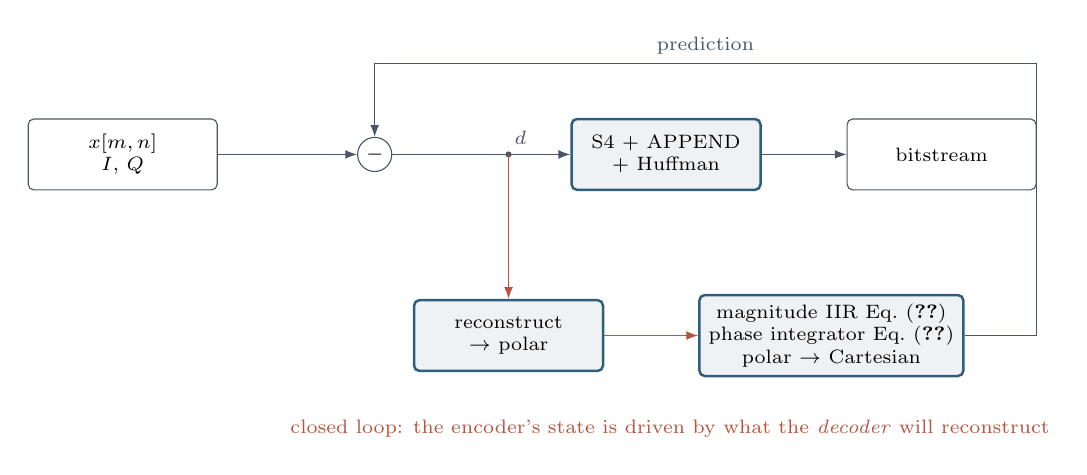
\begin{tikzpicture}[font=\small,
  b/.style={draw=slate,fill=white,rounded corners=2pt,minimum width=24mm,minimum height=9mm,font=\scriptsize,align=center},
  h/.style={b,draw=accent,line width=0.9pt,fill=lightbg},
  s/.style={draw=slate,circle,inner sep=1.5pt,font=\scriptsize},
  a/.style={-{Latex[length=1.5mm]},slate}]

\node[b] (in)  at (0,0)    {$x[m,n]$\\$I,\,Q$};
\node[s] (sum) at (3.2,0)  {$-$};
\node[h] (enc) at (6.9,0)  {S4 + APPEND\\+ Huffman};
\node[b] (out) at (10.4,0) {bitstream};

\node[h] (rec)  at (4.9,-2.3) {reconstruct\\$\to$ polar};
\node[h] (pred) at (9.0,-2.3) {magnitude IIR Eq.~\eqref{eq:magpred}\\phase integrator Eq.~\eqref{eq:phasepred}\\polar $\to$ Cartesian};

\draw[a] (in)  -- (sum);
\draw[a] (sum) -- node[above,font=\scriptsize,text=slate,pos=0.72]{$d$} (enc);
\draw[a] (enc) -- (out);

% tap the residual down into the reconstruction
\fill[slate] (4.9,0) circle (1.1pt);
\draw[a,warm] (4.9,0) -- (rec);
\draw[a,warm] (rec) -- (pred);

% prediction returns to the summing node from above
\draw[a] (pred.east) -- (11.6,-2.3) -- (11.6,1.15) -- node[above,font=\scriptsize,text=slate]{prediction} (3.2,1.15) -- (sum);

\node[font=\scriptsize,text=warm,anchor=north,align=center] at (6.95,-3.25)
  {closed loop: the encoder's state is driven by what the \emph{decoder} will reconstruct};
\end{tikzpicture}
\caption[DRHE block diagram]{DRHE as implemented. Prediction happens in the
polar domain with two filters matched to the expected behaviour of a
constant-velocity target; the prediction is converted back to Cartesian before
subtraction. The red path is the closed-loop correction of
Section~\ref{sec:defect32768}: the encoder drives its state from what the
decoder will reconstruct, not from the original sample.}
\label{fig:drheblock}
\end{figure}

\subsection{The streaming property}

DRHE has a property that matters more than its compression ratio: it is
\emph{causal and streaming}. Each output depends only on the current sample and
on state carried from ramp $m-1$. Concretely, the implementation holds five
floating-point values per (receive channel, range bin) --- the magnitude
prediction, the previous magnitude, the phase prediction, and the previous two
phases --- and nothing else.

It therefore needs no frame buffer, and it emits its first compressed bits as
soon as the first sample arrives. For a compressor sitting between an FFT and a
memory bus, that is exactly the right shape. Section~\ref{sec:headtohead}
returns to this when weighing DRHE against LPC.

\subsection{The assumption}

DRHE's correctness as a \emph{compressor} --- it is lossless regardless --- is
not in question, but its \emph{effectiveness} rests on one assumption made
implicitly by the indices in Equations~\eqref{eq:magpred}
and~\eqref{eq:phasepred}: that ramp $m-1$ is the slow-time predecessor of ramp
$m$.

Section~\ref{sec:tdm} showed that on a TDM-MIMO cascade it is not.

\section{LPC: linear prediction with Yule--Walker coefficients}
\label{sec:lpc}

\subsection{Autoregressive modelling}

The second algorithm takes a more general approach. Rather than assuming a
particular signal shape and hand-designing filters for it, it \emph{fits} a
model to the data.

A second-order autoregressive (AR) model says each sample is approximately a
linear combination of the previous two:
\begin{equation}
\label{eq:ar2}
\hat{x}[m] = a_1 x[m-1] + a_2 x[m-2].
\end{equation}
Given a sequence, the coefficients that minimise the mean-square prediction
error satisfy the Yule--Walker equations, which for order two are
\begin{equation}
\begin{bmatrix} R_0 & R_1 \\ R_1 & R_0 \end{bmatrix}
\begin{bmatrix} a_1 \\ a_2 \end{bmatrix}
=
\begin{bmatrix} R_1 \\ R_2 \end{bmatrix},
\end{equation}
where $R_k = \sum_m x[m]x[m-k]$ is the autocorrelation at lag $k$. Solving
directly,
\begin{equation}
\label{eq:yw}
a_1 = \frac{R_1(R_0 - R_2)}{R_0^2 - R_1^2},
\qquad
a_2 = \frac{R_0 R_2 - R_1^2}{R_0^2 - R_1^2}.
\end{equation}

\subsection{Stability}

An AR model whose poles lie outside the unit circle is unstable: prediction
errors grow rather than decay. For order two the stability triangle gives the
conditions
\begin{equation}
\label{eq:stability}
|a_2| < 1
\qquad\text{and}\qquad
|a_1| < 1 - a_2 .
\end{equation}
If either fails, or if the denominator $R_0^2 - R_1^2$ vanishes, the
implementation sets $a_1 = a_2 = 0$, which degrades gracefully to ``predict
zero'' --- i.e.\ code the raw value. On the real data used here the test never
fires: \SI{100.00}{\percent} of coefficient sets pass.

\subsection{Granularity and side information}

The model is fitted per \emph{(range bin, receive channel, real/imaginary
part)}, across all ramps of the frame. That granularity is a deliberate
compromise: fitting one model to the whole frame would ignore that different
range bins contain targets at different velocities, while fitting per (bin,
ramp) would have no data to fit to.

The coefficients are side information: the decoder cannot reproduce them, so
they must be transmitted. Two 16-bit values per (bin, channel, part) is
\begin{equation}
128 \times 4 \times 2 \times 2 \times 16 = \num{32768}\ \text{bits}
\end{equation}
per frame, which is \SI{1.04}{\percent} of the uncompressed frame. That is a
small but real tax, and Section~\ref{sec:predaxisresults} shows a variant where
it becomes the dominant cost and sinks the whole approach.

\subsection{The cost: LPC is not causal}

$R_0$, $R_1$ and $R_2$ are sums over \emph{all} ramps of the frame. The
coefficients therefore cannot be known until the frame is complete, and the
compressor cannot emit a single bit before then. Where DRHE holds five values
per (channel, bin), LPC must buffer the entire frame:
$4 \times 192 \times 128 \times 32 = \SI{3.1}{\mebi bit}$.

This is the fundamental trade between the two algorithms, and
Section~\ref{sec:headtohead} argues it matters more than the difference in
compression ratio.

\section{Side-by-side}

\begin{table}[t]
\centering
\caption[DRHE and LPC compared]{The two algorithms compared on assumptions and
structure, before any measurement.}
\label{tab:algcompare}
\small
\begin{tabular}{@{}p{38mm}p{45mm}p{45mm}@{}}
\toprule
& \textbf{DRHE} & \textbf{LPC} \\
\midrule
Prediction domain & polar (magnitude, phase) & Cartesian, $I$ and $Q$
  independently \\[3pt]
Model & fixed IIR filters, coefficients $\alpha,\beta$ chosen a priori &
  second-order AR, coefficients fitted per frame \\[3pt]
What it assumes & constant magnitude, constant phase increment &
  the sequence is well described by an order-2 AR process \\[3pt]
Causal? & yes --- streaming, first output immediate & \textbf{no} --- needs the
  whole frame before any output \\[3pt]
State & 5 values per (channel, bin) & \SI{3.1}{\mebi bit} frame buffer \\[3pt]
Side information & none & \num{32768} bits/frame (\SI{1.04}{\percent}) \\[3pt]
Per-sample arithmetic & 4 floating-point transcendentals
  (\texttt{sqrt}, \texttt{atan2}, \texttt{sin}, \texttt{cos}) &
  2 fixed-point multiply--accumulates \\[3pt]
Entropy back end & \multicolumn{2}{c}{identical: S4 + APPEND + fixed Huffman} \\
\bottomrule
\end{tabular}
\end{table}

Table~\ref{tab:algcompare} summarises. The expectation going in --- stated
explicitly here so that Chapter~\ref{ch:results} can be checked against it ---
was that LPC would compress slightly better, because a fitted model should beat
a fixed one, but would be the expensive design, because it contains a division
and DRHE does not. Exactly one half of that expectation survived measurement.

% ===================================================================
\chapter{Methodology}
\label{ch:method}

\section{The verification ladder}
\label{sec:ladder}

A compression algorithm that is \emph{nearly} lossless is useless, so the
method has to be able to prove exactness rather than estimate it. The approach
taken is a ladder of four phases, each one validating the phase above it at a
lower level of abstraction. The key property is that each rung has a
\emph{reference} it can be checked against, so a discrepancy always localises
to one transition.

\begin{figure}[t]
\centering
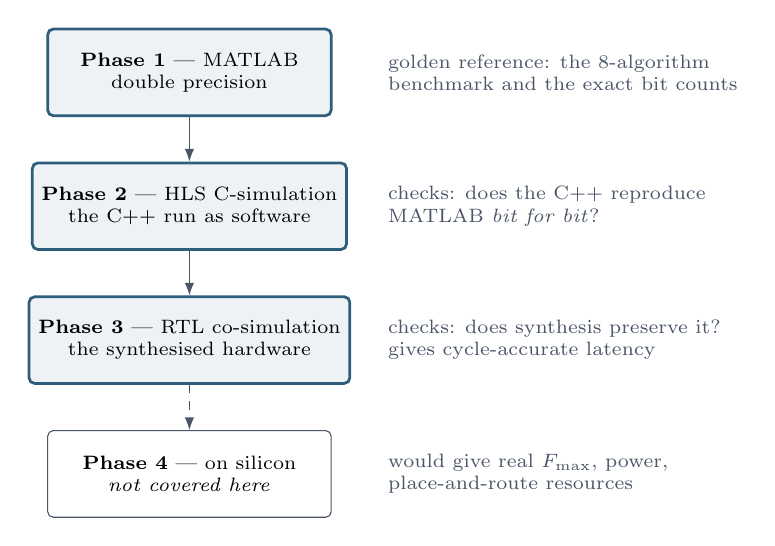
\begin{tikzpicture}[font=\small,
  ph/.style={draw=slate,fill=white,rounded corners=2pt,minimum width=36mm,minimum height=11mm,align=center,font=\scriptsize},
  hl/.style={ph,draw=accent,line width=1pt,fill=lightbg},
  a/.style={-{Latex[length=1.6mm]},slate}]
\node[hl] (p1) at (0,0) {\textbf{Phase 1} --- MATLAB\\double precision};
\node[hl] (p2) at (0,-1.7) {\textbf{Phase 2} --- HLS C-simulation\\the C++ run as software};
\node[hl] (p3) at (0,-3.4) {\textbf{Phase 3} --- RTL co-simulation\\the synthesised hardware};
\node[ph]  (p4) at (0,-5.1) {\textbf{Phase 4} --- on silicon\\\emph{not covered here}};
\draw[a] (p1) -- (p2); \draw[a] (p2) -- (p3); \draw[a,dashed] (p3) -- (p4);
\node[font=\scriptsize,text=slate,anchor=west,align=left] at (2.4,0)
  {golden reference: the 8-algorithm\\benchmark and the exact bit counts};
\node[font=\scriptsize,text=slate,anchor=west,align=left] at (2.4,-1.7)
  {checks: does the C++ reproduce\\MATLAB \emph{bit for bit}?};
\node[font=\scriptsize,text=slate,anchor=west,align=left] at (2.4,-3.4)
  {checks: does synthesis preserve it?\\gives cycle-accurate latency};
\node[font=\scriptsize,text=slate,anchor=west,align=left] at (2.4,-5.1)
  {would give real $F_{\max}$, power,\\place-and-route resources};
\end{tikzpicture}
\caption[The four-phase verification ladder]{The verification ladder. Each
phase is checked against the one above it, so a mismatch localises to a single
transition rather than to ``somewhere in the design''.}
\label{fig:ladder}
\end{figure}

\paragraph{Phase 1 --- MATLAB.}
The entire radar chain is modelled in double precision, and all eight
compression schemes are run against it. This establishes the golden reference:
the exact FX16 values, the exact number of bits each algorithm should produce,
and the detection metrics.

\paragraph{Phase 2 --- HLS C-simulation.}
Because the hardware design is written in C++, it can be compiled and executed
as ordinary software. This phase asks one question: does the C++ produce
\emph{exactly} the bits that MATLAB says it should, and does the decompressor
recover \emph{exactly} the original samples? It runs in minutes over all 50
frames, which makes it the workhorse of the whole project.

\paragraph{Phase 3 --- RTL co-simulation.}
The C++ is synthesised to Verilog and the same testbench is re-run with the
generated RTL substituted for the software. This checks that synthesis
preserved behaviour --- pipelining, array partitioning and fixed-point
inference can all change results if a design is subtly wrong --- and returns a
cycle-accurate latency figure that no software simulation can give.

\paragraph{Phase 4 --- silicon.}
Out of scope here; it requires the physical board. Every hardware number in this
thesis is therefore a synthesis or co-simulation \emph{estimate}, which
Section~\ref{sec:threats} restates as a limitation.

\section{The reference signal chain}
\label{sec:refchain}

The MATLAB chain is described here in the order it executes, because several
later observations depend on details of individual steps.

\subsection{Loading}
A frame is read from the ColoRadar binary and reshaped into a complex cube of
(fast time $\times$ ramp $\times$ receiver), with the TDM flattening of
Equation~\eqref{eq:rampindex}. The per-ramp mean is subtracted from each
channel to remove the DC / transmitter-leakage term.

\subsection{Windowing}
A Hann window is applied along fast time to suppress spectral leakage, so that
a strong nearby target does not bury a weak distant one in sidelobes.

\subsection{Range FFT}
An $N_s$-point FFT is taken along fast time and normalised by $N_s$. Only the
positive half-spectrum is retained, giving $N = 128$ range bins. This halving
is a deliberate choice, not a consequence of conjugate symmetry --- the input
here is complex $I/Q$, so the spectrum is \emph{not} symmetric; the negative
half corresponds to negative beat frequencies, which are not physically
meaningful ranges.\footnote{A code comment in the reference implementation
described this as a symmetry consequence. It is not, and the comment has been
corrected.}

\subsection{FX16 quantisation}
The complex FFT output is scaled by Equation~\eqref{eq:scale} and rounded to
\texttt{int16}. This is the last step before compression, and its output ---
128 range bins $\times$ 192 ramps $\times$ 4 receive channels of complex
\texttt{int16} --- is exactly what both compressors consume.

Four receive channels rather than sixteen are exported to the hardware path,
because four complex \texttt{int16} samples is \num{128} bits, the AXI4-Stream
width. Section~\ref{sec:threats} notes the consequence for comparisons against
the 16-channel MATLAB benchmark.

\subsection{Detection and metrics}
The reconstructed data is put through Doppler and angle processing and a
threshold detector, and the resulting detections are compared against those
from the double-precision reference. The threshold is the mean of the lowest
\SI{75}{\percent} of sorted magnitudes plus a fixed \SI{15}{\decibel} offset,
with 8-connected local-maximum suppression.

\section{Metrics, defined precisely}
\label{sec:metrics}

Several metric names are used loosely in this field. They are pinned down here.

\subsection{Compression ratio}
\begin{equation}
\mathrm{CR} = \frac{B_{\mathrm{in}}}{B_{\mathrm{out}}},
\qquad
B_{\mathrm{in}} = N_{\mathrm{ramps}} \times N \times N_{\mathrm{RX}} \times 32,
\end{equation}
with $B_{\mathrm{out}}$ the compressed length \emph{including} AXI packet
padding. Including the padding matters: a design that flushed its bit buffer
per ramp rather than per frame would waste up to 255 bits per ramp, costing
about \SI{2.9}{\percent} of the ratio. Reporting the ratio without padding
would hide that design choice.

\subsection{Maximum absolute difference}
\begin{equation}
\mathrm{MaxDiff} = \max_{\text{all samples}}
   \bigl| x - \tilde{x} \bigr|
\end{equation}
over every real and imaginary component. For a lossless coder the pass
criterion is $\mathrm{MaxDiff} = 0$. There is no tolerance.

\subsection{Detection metrics, and one correction}
\label{sec:detectionmetrics}

Let $D_{\mathrm{ref}}$ be the detection set from the double-precision reference
and $D_{\mathrm{test}}$ that from the reconstructed data. The two rates reported
are
\begin{equation}
\mathrm{FN}\% = \frac{|D_{\mathrm{ref}} \setminus D_{\mathrm{test}}|}{|D_{\mathrm{ref}}|},
\qquad
\mathrm{FP}\% = \frac{|D_{\mathrm{test}} \setminus D_{\mathrm{ref}}|}{|D_{\mathrm{test}}|}.
\end{equation}

The first is a false negative rate in the ordinary sense. The second is
\textbf{not} a false positive rate, despite the label it carries in the
literature and in this author's own earlier reporting. A false positive rate
normalises by the number of true negatives --- in a range--Doppler map, the
number of empty cells. This quantity normalises by the number of \emph{test
detections}, which makes it a \textbf{false discovery rate}. It is a perfectly
legitimate metric, and arguably the more useful one here, but it is not what
its conventional name denotes. It is reported under its correct name throughout
this thesis.

Two further properties bound how much weight the detection metrics can carry,
and are stated rather than buried:

\begin{itemize}
\item \textbf{The comparison is cell-wise and exact.} A target detected one
range--Doppler cell away from its reference position counts as both a false
negative \emph{and} a false discovery. There is no positional tolerance, which
inflates both rates relative to a matched-detection criterion.
\item \textbf{The \SI{15}{\decibel} threshold is a free parameter.} It is not
swept, and the detection rates are sensitive to it.
\end{itemize}

\subsection{What the detection metrics actually measure here}

This point is important enough to state on its own. FX16, DRHE and LPC are all
exactly lossless \emph{with respect to the FX16 codes}. Their reconstructed
data is bit-identical, so their detection metrics are identical \emph{by
construction} --- not by coincidence, and not as evidence that the compressors
are equally good.

What the detection metrics measure in this thesis is therefore the cost of the
\textbf{FX16 quantisation step}, which is the only lossy operation in the
lossless chain. They are reported for that purpose, and to provide the contrast
against the genuinely lossy BAQ.

\subsection{Order-0 entropy}
To judge the entropy coder rather than the whole compressor,
Equation~\eqref{eq:entropy} is evaluated empirically on the residual
distribution. The gap between the entropy and the achieved bits per value is
the coder's inefficiency; the entropy itself is the figure of merit for the
\emph{predictor}.

This is the measurement that exposed the central finding, and it is worth
noting that it is not a standard part of a compression evaluation. Had it not
been made, the prediction-axis error would have remained invisible behind a
respectable-looking compression ratio.

\section{Edge-case testing}
\label{sec:edgecases}

Real data exercises the typical case well and the extreme case not at all. The
ColoRadar residuals span roughly $[-514, +416]$, which is entirely inside
category 10 of a 16-category code. Everything above that was, until deliberately
tested, unexercised.

An eight-case synthetic testbench was therefore built
(Table~\ref{tab:edgecases}), generating its stimulus internally so that it runs
identically in C-simulation and co-simulation.

\begin{table}[t]
\centering
\caption[Synthetic edge cases]{The synthetic edge-case suite. Each case has its
own allowed reconstruction error --- zero for all but the two that exercise the
saturation described in Section~\ref{sec:defect32768}.}
\label{tab:edgecases}
\small
\begin{tabular}{@{}llc@{}}
\toprule
Case & What it exercises & Allowed $\mathrm{MaxDiff}$ \\
\midrule
all-zeros        & the $S_4 = 0$ path and the best case & 0 \\
dc-constant      & a perfectly predictable sequence & 0 \\
random-int16     & the worst case: incompressible input & 0 \\
tone-192ramp     & a periodic sequence the AR model should fit & 0 \\
tone-1ramp       & a sequence too short to fit & 0 \\
max-amplitude    & full-scale values, and 128-bit correlations & 0 \\
max-alternating  & $\pm 32767$ alternating: the largest residuals & 1 \\
int16-min        & $-32768$ specifically & 1 \\
\bottomrule
\end{tabular}
\end{table}

Both defects reported in Section~\ref{sec:defects} were found by this suite and
by nothing else. Neither is reachable with real radar data. The general lesson
--- that dataset-driven verification and adversarial synthetic verification
find different classes of bug and neither substitutes for the other --- is
returned to in Section~\ref{sec:lessons}.

\section{Toolchain and reproducibility}

All MATLAB work used R2024b with the Signal Processing Toolbox. All hardware
work used AMD Vitis HLS 2026.1 targeting \texttt{xcku5p-ffvb676-2-e} at a
\SI{100}{\mega\hertz} clock, with a licensed Vivado installation for synthesis
and XSIM for co-simulation.

Two practical points are recorded because they cost time. First, Vitis refuses
to create a project under a path containing a space, so the build tree must
live somewhere like \texttt{D:\textbackslash Thesis} rather than under a user
directory whose name contains one. Second, the stimulus for the hardware
testbenches is exported \emph{from MATLAB as \texttt{int16}} rather than
recomputed in C++. This eliminates any possibility of a floating-point FFT
discrepancy between the two environments: the C++ testbench and the MATLAB
reference operate on byte-identical input, so any difference in output is
unambiguously a difference in the compressor.

% ===================================================================
\chapter{Implementation}
\label{ch:implementation}

\section{Common infrastructure}

Both compressors present the same interface: AXI4-Stream in at \num{128} bits
per beat (four channels of 16-bit $I$ and $Q$), AXI4-Stream out at \num{256}
bits per beat of compressed bitstream, with the frame dimensions
($N$, $N_{\mathrm{ramps}}$, $N_{\mathrm{RX}}$, and for the corrected variants
$n_{\mathrm{Tx}}$) on an AXI4-Lite control bundle.

Both share the bit-packing arrangement. Codewords accumulate into a 512-bit
register, least-significant-bit first, and a 256-bit AXI word is flushed
whenever at least 256 bits are available, with a final partial flush at end of
frame. Flushing per frame rather than per ramp is what avoids the
\SI{2.9}{\percent} padding penalty noted in Section~\ref{sec:metrics}.

The Huffman codewords are stored bit-reversed relative to the published
dictionary, because the packer is LSB-first. The reversed code set remains
prefix-free, so the decoder can match candidates from the low end of its buffer
without ambiguity --- at most one table entry can match.

\section{DRHE architecture}
\label{sec:drheimpl}

\subsection{State and parallelism}

DRHE holds five \texttt{float} arrays of shape
$[N_{\mathrm{RX}}][N]$: the magnitude prediction, the previous magnitude, the
phase prediction, and the previous two phases. The channel dimension is
completely partitioned, so the four receive channels are four parallel copies
of the datapath inside one pipelined iteration of the sample loop --- the
parallelism argument of Section~\ref{sec:fpga} made concrete.

State is zeroed on the first ramp of each frame. This makes frames independent:
a frame lost in transit cannot corrupt its successors, which is a desirable
property for a streaming sensor and one that the 50-frame test confirms
directly.

\subsection{Why it is expensive}

Per sample, per channel, DRHE evaluates \texttt{sqrt} and \texttt{atan2} to get
polar coordinates, then \texttt{sin} and \texttt{cos} to get back. Four
floating-point transcendental functions, four times over for four channels, on
every one of \num{24576} beats per frame.

Chapter~\ref{ch:results} shows the bill: these functions account for the bulk
of \num{115534} LUTs, and the resulting combinational depth is why the design
estimates \SI{81.88}{\mega\hertz} rather than meeting its \SI{100}{\mega\hertz}
target. Replacing them with a fixed-point CORDIC would be the obvious
optimisation and is left as future work.

\subsection{The initiation-interval bottleneck}

DRHE achieves $\mathrm{II} = 2$ rather than the target $\mathrm{II} = 1$, and
the reason is instructive because it has nothing to do with arithmetic.

Each state array is partitioned on the channel dimension, so each channel's
$[N]$ history is one dual-port block RAM. Every iteration reads a value from it
and writes the updated value back --- two accesses, which two ports can just
manage. But on the first ramp the iteration \emph{also} writes a reset value.
Three accesses against two ports forces the tool to serialise, and the loop
settles at $\mathrm{II} = 2$ for the whole frame on account of a condition that
is true for one ramp in 192.

The fix is straightforward --- hoist the reset into its own unpipelined loop
before the main one, or partition cyclically on the bin dimension as well ---
and would roughly double throughput. It is identified rather than implemented
here.

\section{LPC architecture}
\label{sec:lpcimpl}

\subsection{Three passes}

LPC cannot stream, so its structure is explicitly multi-pass
(Figure~\ref{fig:lpcblock}):

\begin{enumerate}
\item \textbf{Ingest.} Read the frame into the buffer, accumulating $R_0$,
$R_1$, $R_2$ per (channel, bin) as the samples arrive.
\item \textbf{Solve and residual.} For each (channel, bin), solve
Equation~\eqref{eq:yw}, then walk the ramps again computing residuals and
rewriting the buffer \emph{in place}.
\item \textbf{Emit.} Write the coefficient table, then the residuals.
\end{enumerate}

Rewriting the buffer in place matters: it means one \SI{3.1}{\mebi bit} memory
serves both purposes rather than two.

\begin{figure}[t]
\centering
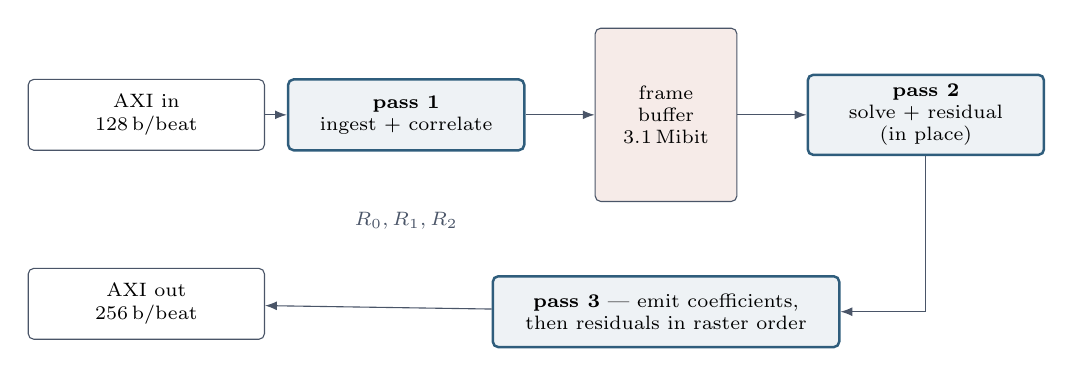
\begin{tikzpicture}[font=\small,
  b/.style={draw=slate,fill=white,rounded corners=2pt,minimum width=30mm,minimum height=9mm,font=\scriptsize,align=center},
  h/.style={b,draw=accent,line width=0.9pt,fill=lightbg},
  m/.style={draw=slate,fill=warm!12,rounded corners=2pt,minimum width=18mm,minimum height=22mm,font=\scriptsize,align=center},
  a/.style={-{Latex[length=1.5mm]},slate}]
\node[b]  (in)  at (0,0)    {AXI in\\128\,b/beat};
\node[h]  (p1)  at (3.3,0)  {\textbf{pass 1}\\ingest + correlate};
\node[m]  (buf) at (6.6,0)  {frame\\buffer\\\SI{3.1}{\mebi bit}};
\node[h]  (p2)  at (9.9,0)  {\textbf{pass 2}\\solve + residual\\(in place)};
\node[h,minimum width=44mm]  (p3)  at (6.6,-2.5) {\textbf{pass 3} --- emit coefficients,\\then residuals in raster order};
\node[b]  (out) at (0,-2.4) {AXI out\\256\,b/beat};
\draw[a] (in) -- (p1);
\draw[a] (p1) -- (buf);
\draw[a] (buf) -- (p2);
\draw[a] (p2.south) -- (9.9,-2.5) -- (p3.east);
\draw[a] (p3) -- (out);
\node[font=\scriptsize,text=slate,align=center] at (3.3,-1.35) {$R_0,R_1,R_2$};
\end{tikzpicture}
\caption[LPC three-pass architecture]{The LPC compressor. Because the
Yule--Walker coefficients depend on the whole frame, the compressor must buffer
it; the buffer is then rewritten in place with residuals so that only one
memory is needed. Emitting residuals in the original raster order is what lets
the \emph{decompressor} avoid a frame buffer entirely.}
\label{fig:lpcblock}
\end{figure}

\subsection{A useful asymmetry}

Pass 3 emits the coefficient table first --- the decoder needs all of it before
it can reconstruct anything --- and then the residuals \emph{in the same raster
order the samples arrived in}, rather than in the (channel, bin, ramp) order
pass 2 produced them.

The payoff is that the decompressor needs no frame buffer at all. It holds the
coefficient table and two reconstructed samples per (channel, bin) --- the same
\emph{shape} of state DRHE uses --- and writes each output sample as its
residual arrives. The reordering cost is paid once, by the side that already
had to buffer.

This is worth noting because it inverts the usual expectation. LPC's
non-causality is a compressor-side problem only; at the receiving SoC, where
memory is comparatively plentiful but latency still matters, LPC decompression
is as cheap as DRHE's.

\subsection{Fixed-point choices}

Coefficients are quantised to \texttt{ap\_fixed<16,2>} for $a_1$ (range
$[-2,2)$) and \texttt{ap\_fixed<16,1>} for $a_2$ (range $[-1,1)$), which
follows from the stability conditions of Equation~\eqref{eq:stability}.
Measured over 50 frames, this quantisation costs \SI{0.0000}{\percent} of
compression ratio relative to double-precision coefficients --- the residuals
are unchanged to the bit. The fitted models are evidently not sensitive at that
level, which retrospectively justifies the 16-bit side-information budget.

The autocorrelations are accumulated as exact 64-bit integers rather than in
floating point. This is deliberate: $R_0^2 - R_1^2$ is a difference of two
nearly equal quantities whenever the data is strongly correlated --- precisely
the regime the predictor exists for --- so computing it in floating point would
lose most of its significant digits exactly when accuracy matters most. Forming
all three 128-bit quantities exactly in integer arithmetic before any division
avoids the cancellation entirely.

\section{Two defects found and fixed}
\label{sec:defects}

Both defects described here share a pattern worth naming: each was invisible on
real data, each was found by a synthetic edge case, and each would have
shipped.

\subsection{Defect 1: the \texorpdfstring{$-32768$}{-32768} residual}
\label{sec:defect32768}

\paragraph{Symptom.}
The \texttt{max-alternating} edge case --- input alternating $\pm 32767$ ---
produced $\mathrm{MaxDiff} = \num{65535}$. That number is diagnostic: it is
exactly the distance from $-32768$ to $+32767$, which points straight at the
representability hole of Section~\ref{sec:hole}. Instrumenting the encoder
confirmed it:
\begin{verbatim}
MISMATCH v=-32768  s4=15  append=0x7FFF  decoded=32767
\end{verbatim}

\paragraph{The three possible fixes.}
\begin{enumerate}
\item \textbf{Extend the code with a category 16.} Correct in general, but it
changes the bitstream format and breaks compatibility with the reference
design's dictionary.
\item \textbf{Reject the input.} Legitimate for a closed system but unhelpful
for a general IP core.
\item \textbf{Saturate $-32768$ to $-32767$.} Costs at most one LSB on the
affected sample and leaves the format untouched.
\end{enumerate}
Option 3 was chosen. On real data the clamp never fires, since residuals span
roughly $[-514, +416]$, so behaviour on the dataset is unchanged.

\paragraph{Why saturation alone is not enough.}
Saturation makes the reconstruction differ from the original by one LSB, and
that is where Section~\ref{sec:closedloop} becomes concrete. The encoder
originally derived its next prediction from the \emph{original} sample, while
the decoder necessarily derives it from the \emph{reconstructed} one. These
agree only while reconstruction is exact. The moment the clamp fires they
diverge --- and because Equations~\eqref{eq:magpred} and~\eqref{eq:phasepred}
are IIR filters, that divergence is then carried forward through every
remaining ramp of the frame, growing rather than decaying.

The complete fix is therefore to close the loop. The encoder reconstructs
exactly what the decoder will produce and drives its state from that:

\begin{verbatim}
int diff_re = wrap_int16(re - pred_re);
if (diff_re == -32768) diff_re = -32767;      // saturate
int recon_re = wrap_int16(diff_re + pred_re); // what the decoder will see
float curr_mag   = hls::sqrt(recon_re*recon_re + recon_im*recon_im);
float curr_phase = hls::atan2(recon_im, recon_re);   // state from recon
\end{verbatim}

\paragraph{The cost.}
Where reconstruction is exact --- which is everywhere on real data --- the
closed-loop and open-loop forms are identical by construction, so compression
is unchanged. The cost falls entirely on synthesis: the reconstruction now sits
on the dependency chain ahead of the polar conversion, so pipeline depth rises
from \num{32} to \num{58} cycles and registers from \num{40309} to
\num{57105}. Initiation interval and $F_{\max}$ are unaffected.

That is a real price --- Section~\ref{sec:kiemcompare} notes that it roughly
doubles the IP-core latency --- and it is the direct cost of bounding an error
that cannot occur on this dataset but could occur on another. Option 1 above
would avoid it, at the price of bitstream compatibility.

\subsection{Defect 2: 128-bit to float conversion}
\label{sec:defect128}

\paragraph{Symptom.}
The \texttt{max-amplitude} edge case produced wrong coefficients. Tracing
showed a determinant of $4.4\times10^{20}$ converting to
$-1.2\times10^{18}$ --- not merely imprecise but the wrong sign.

\paragraph{Cause.}
Equation~\eqref{eq:yw} needs products of 64-bit correlations, so the numerators
and the determinant are computed as \texttt{ap\_int<128>}. Converting such a
value directly to \texttt{float} is not correct above $2^{64}$ in this
toolchain: \texttt{(float)(1 << 70)} evaluates to zero.

\paragraph{Fix.}
Normalise all three operands by a common arithmetic right shift into 62 bits
before the division, choosing the shift from the largest of the three:
\begin{equation}
k = \max\bigl(\mathrm{msb}|D|,\ \mathrm{msb}|N_1|,\ \mathrm{msb}|N_2|\bigr) - 61,
\end{equation}
clamped at zero. Because the same shift is applied to numerator and
denominator, the quotient is mathematically unchanged; only the intermediate
representation is brought into a range the conversion handles.

\paragraph{Why it was invisible.}
On real ColoRadar data the correlations reach only 44 bits, comfortably inside
the range where the conversion is correct. The defect is unreachable with this
dataset and would have been unreachable with any similarly scaled one. It is,
in other words, precisely the class of bug that a dataset-driven test plan
cannot find.

\section{The TDM-aware variants}
\label{sec:tdmimpl}

Chapter~\ref{ch:results} motivates these; this section describes what they are,
since they are implementation rather than result.

\subsection{DRHE}

The change is confined to state indexing. The five state arrays gain a
transmitter dimension, indexed by $m \bmod n_{\mathrm{Tx}}$, and the reset
condition widens from $m = 0$ to $m < n_{\mathrm{Tx}}$, because each
transmitter's history begins on its own first ramp rather than on the frame's.
The prediction equations, the coefficients, the residual computation, the
entropy coder and the bitstream format are all untouched.

The state grows by a factor $n_{\mathrm{Tx}}$ in principle. In practice the
baseline was dimensioned for up to \num{1024} range bins and the corrected
version for the \num{128} actually used, so the realised growth is
$1.5\times$: from \num{40} to \num{80} block RAMs.

Crucially, the \emph{schedule} does not change. Indexing the state by
transmitter changes which address is read, not when, so the initiation
interval, the pipeline depth and the frame latency are all identical. The
correction is therefore close to free.

\subsection{LPC, and a ring buffer trick}

LPC needs more work, because both the autocorrelation and the residual pass now
need $x[m - n_{\mathrm{Tx}}]$ and $x[m - 2n_{\mathrm{Tx}}]$ rather than
$x[m-1]$ and $x[m-2]$.

A naive shift register of depth $2n_{\mathrm{Tx}} = 24$ would shift 24 entries
every iteration. Instead, observe that a \emph{ring} of exactly
$2n_{\mathrm{Tx}}$ entries gives both taps for free. At ramp $m$, let
$k = m \bmod 2n_{\mathrm{Tx}}$. Slot $k$ still holds the value written at ramp
$m - 2n_{\mathrm{Tx}}$, because it is about to be overwritten and has not been
touched since; and slot $(k + n_{\mathrm{Tx}}) \bmod 2n_{\mathrm{Tx}}$ holds
the value from ramp $m - n_{\mathrm{Tx}}$, since that is the most recent ramp
congruent to $k + n_{\mathrm{Tx}}$. So:
\begin{center}
\begin{tabular}{@{}ll@{}}
read $x[m-2n_{\mathrm{Tx}}]$ & from slot $k$ \\
read $x[m-n_{\mathrm{Tx}}]$  & from slot $(k+n_{\mathrm{Tx}}) \bmod 2n_{\mathrm{Tx}}$ \\
write $x[m]$                 & to slot $k$ \\
\end{tabular}
\end{center}
Nothing is shifted; the cost is $2n_{\mathrm{Tx}}$ registers and two
multiplexers.

\subsection{A restructure that pays for itself}

Accumulating the autocorrelations during ingest is no longer convenient at the
deeper lags, so they were moved into the per-bin pass instead, computed from the
frame buffer through the ring above. This deleted six 64-bit accumulator arrays
and four history arrays outright.

The consequences, quantified in Chapter~\ref{ch:results}, are mixed and
interesting: block RAM usage \emph{falls} by \SI{25}{\percent}, and the ingest
loop --- previously stuck at $\mathrm{II} = 3$ on accumulator port pressure ---
now meets $\mathrm{II} = 1$, as does every other loop in the design. Against
that, the design now makes two short passes over each (channel, bin) instead of
one long one, and Section~\ref{sec:tdmresults} shows that the pipeline drain
this incurs costs considerably more than a naive cycle model predicts.

\subsection{Both baselines retained}

The original DRHE and LPC designs were kept alongside the corrected ones rather
than replaced. This is deliberate: it allows a like-for-like comparison at every
level, and it means the results in Chapter~\ref{ch:results} are differences
measured on the same machine with the same toolchain on the same day, not
comparisons against remembered numbers.

% ===================================================================
\chapter{Results}
\label{ch:results}

This chapter reports what was measured. It is arranged so that the story
unfolds in the order it actually did: first the benchmark and the verification,
which all passed and all looked satisfactory; then the audit that asked what the
numbers meant and found they did not mean what they appeared to; then the
correction and its consequences.

\section{Phase 1: the MATLAB benchmark}
\label{sec:phase1}

\subsection{Eight algorithms on real data}

Table~\ref{tab:phase1} gives the 50-frame average over \num{9934} reference
detections, using all 16 receive channels. The reference against which
everything is compared is the double-precision path, so FP16 --- half-precision
floating point --- registers as effectively lossless.

\begin{table}[t]
\centering
\caption[Phase 1 benchmark]{Phase 1: eight compression schemes, 50-frame
average, 16 receive channels, \num{9934} reference detections. FP\% is a false
discovery rate (Section~\ref{sec:detectionmetrics}). NF is the noise floor.}
\label{tab:phase1}
\small
\begin{tabular}{@{}lrrrrr@{}}
\toprule
Algorithm & CR & FN\% & FP\% & NF (dBFS) & SNR (dB)\\
\midrule
FP16          & 1.00 & 0.00  & 0.00 & $-105.638$ & 35.504\\
DRHEfp16      & 1.04 & 0.05  & 0.01 & $-105.637$ & 35.505\\
FX16          & 1.00 & 3.77  & 1.11 & $-105.374$ & 35.359\\
\textbf{DRHE} & \textbf{3.30} & 3.77 & 1.11 & $-105.374$ & 35.359\\
BAQ           & 3.76 & 10.44 & 9.69 & $-105.080$ & 35.081\\
RDVLE         & 1.12 & 24.01 & 4.62 & $-102.275$ & 33.165\\
RDVLE\_UDRE   & 2.56 & 28.73 & 4.44 & $-101.782$ & 33.004\\
\textbf{LPC}  & \textbf{3.37} & 3.77 & 1.11 & $-105.374$ & 35.359\\
\bottomrule
\end{tabular}
\end{table}

Three things are worth drawing out.

\paragraph{The lossless coders share FX16's detection metrics exactly.}
FX16, DRHE and LPC report identical FN\%, FP\%, noise floor and SNR. As
Section~\ref{sec:detectionmetrics} explained, this is not a coincidence but a
tautology: all three reconstruct the FX16 codes bit-exactly, so the detector
sees identical data. What the table is really showing in those rows is the cost
of \emph{quantisation}, which is \SI{3.77}{\percent} of detections missed and
\SI{1.11}{\percent} of reported detections spurious.

\paragraph{The lossy comparison is instructive.}
BAQ reaches a nominally better ratio --- \num{3.76} against \num{3.30} --- but
misses \SI{10.44}{\percent} of detections instead of \SI{3.77}{\percent}, and
\SI{9.69}{\percent} of what it does report is spurious against
\SI{1.11}{\percent}. That is nearly three times the miss rate and nearly nine
times the false discovery rate, for a \SI{14}{\percent} improvement in ratio.
In a system that brakes the car, that is not a trade anyone should take. This
is the empirical form of the argument made on principle in
Section~\ref{sec:lossless}.

\paragraph{The predictive coders reach the target.}
DRHE's \num{3.30} matches the \num{3.2} reported for the baseline design
\cite{kiem2025}, which at the time was taken as confirmation that the
implementation was correct. Section~\ref{sec:decomposition} revisits that
interpretation.

\section{Phase 2: bit-exactness}
\label{sec:phase2}

\subsection{The headline}

Over 50 frames --- \num{157286400} complex samples --- both HLS
implementations reconstruct every sample of every frame exactly:
$\mathrm{MaxDiff} = 0$, mean squared error $= 0$, signal-to-noise ratio
infinite. Compression ratios are \num{3.30987} for DRHE and \num{3.38497} for
LPC.

\subsection{How closely the hardware matches MATLAB}

Agreement with the MATLAB reference is an order of magnitude tighter than the
$\pm 0.01$ criterion set in advance.

For LPC the agreement is exact. A MATLAB model that charges the same 256-bit
AXI padding reproduces the Vitis bit count on \num{50} of \num{50} frames to
within $4.9\times 10^{-6}$ --- which means the entire discrepancy between the
two is packet padding and the underlying bit counts are identical.

\begin{table}[t]
\centering
\caption[LPC MATLAB-versus-hardware agreement]{LPC, mean compression ratio over
50 frames, computed four ways. The padding model reproduces the hardware result
on every frame, so the HLS bit counts are bit-exact with MATLAB.}
\label{tab:lpcagree}
\small
\begin{tabular}{@{}lr@{}}
\toprule
Quantity & Value \\
\midrule
MATLAB, double-precision coefficients & \num{3.38541} \\
MATLAB, 16-bit quantised coefficients & \num{3.38541} \\
\quad (quantisation cost) & \SI{0.0000}{\percent} \\
MATLAB, quantised + 256-bit AXI padding & \textbf{\num{3.38497}} \\
\textbf{Vitis HLS, measured} & \textbf{\num{3.38497}} \\
\midrule
Frames where the padding model matches & \num{50} / \num{50} \\
Worst-frame difference & \num{0.00091} (tolerance $\pm 0.01$) \\
\bottomrule
\end{tabular}
\end{table}

For DRHE the hardware bit count exceeds the MATLAB count by between \num{15}
and \num{252} bits per frame, mean \num{134}. That range sits strictly inside
one 256-bit packet, which is exactly what a per-frame flush should produce, so
again the residual difference is padding rather than disagreement.

\subsection{Edge cases}

All eight synthetic cases of Table~\ref{tab:edgecases} pass for both coders
after the fixes of Section~\ref{sec:defects}. Two results are worth recording
because they were initially misread as failures:

\begin{itemize}
\item \textbf{\texttt{random-int16} compresses to \num{0.60}} --- that is,
it \emph{expands} the data by \SI{67}{\percent}. This is correct behaviour, not
a bug. Incompressible input has no structure to remove, and every residual
lands in a high category costing a 12-bit codeword plus 15 APPEND bits. Every
lossless coder expands incompressible input; it is a theorem that some input
must.
\item \textbf{\texttt{tone-192ramp} reaches only \num{1.10} under LPC.} The
synthetic tone's period is about \num{209} ramps, longer than the \num{192}-ramp
frame, so the autocorrelation estimate is poor and the fitted coefficients are
$a_1 = 1.0377$, $a_2 = -0.0484$ against the ideal $a_1 = 2\cos\omega = 1.9991$,
$a_2 = -1$. MATLAB's solver produces the same coefficients, and its stability
test does not fire either, so this is a property of the second-order
Yule--Walker estimator on a truncated period, not an implementation fault.
\end{itemize}

\section{Phase 3: synthesis and co-simulation}
\label{sec:phase3}

\subsection{Resources}

Table~\ref{tab:resources} gives post-synthesis estimates for both compressors
on the \texttt{xcku5p}.

\begin{table}[t]
\centering
\caption[Synthesis estimates]{Post-synthesis resource and timing estimates,
\texttt{xcku5p} at a \SI{100}{\mega\hertz} target. Percentages are of the
device, which has \num{216960} LUT, \num{433920} FF, \num{960} BRAM\_18K and
\num{1824} DSP. The reference column is Kiem's ZU3EG design \cite{kiem2025},
which is a device roughly three times smaller, so only absolute counts are
comparable.}
\label{tab:resources}
\small
\begin{tabular}{@{}lrrr@{}}
\toprule
Resource & DRHE & LPC & Reference \cite{kiem2025}\\
\midrule
LUT              & \num{115534} (53\%) & \num{80528} (37\%) & \num{45892}\\
FF               & \num{57105} (13\%)  & \num{17393} (4\%)  & \num{9243}\\
BRAM\_18K        & \num{40} (4\%)      & \num{256} (26\%)   & \num{10}\\
DSP              & \num{132} (7\%)     & \num{168} (9\%)    & \num{44}\\
Est.\ $F_{\max}$ & \SI{81.88}{\mega\hertz} & \SI{85.43}{\mega\hertz} & \SI{100}{\mega\hertz}\\
Frame latency    & \num{61253} cyc & \num{197277} cyc & ---\\
Worst loop II    & 2 & 3 & 1\\
Frame buffer     & none & \SI{3.1}{\mebi bit} & ---\\
\bottomrule
\end{tabular}
\end{table}

\subsection{Neither design meets timing}

Both estimate below \SI{100}{\mega\hertz}: \SI{81.88}{\mega\hertz} for DRHE and
\SI{85.43}{\mega\hertz} for LPC. The critical path in DRHE is the chain of
floating-point transcendentals described in Section~\ref{sec:drheimpl}. The
remedy --- pipelining the float datapath, or replacing the polar conversion
with a fixed-point CORDIC --- is identified but not implemented.

\subsection{The expectation that did not survive}

Section~\ref{ch:algorithms} recorded the prior expectation that LPC would be
the expensive design, because it contains a division and DRHE does not.

It is not. LPC uses \SI{30}{\percent} fewer LUTs and \SI{70}{\percent} fewer
flip-flops. The reason is that per-sample cost dominates: LPC's inner loop is
two fixed-point multiply--accumulates, while DRHE's is four floating-point
transcendentals. The division runs \num{1024} times per frame --- once per
(bin, channel, part) --- and contributes \num{512} cycles out of \num{197277},
or \SI{0.26}{\percent}. It is not the bottleneck by any measure.

What LPC costs instead is \emph{memory and latency}. Its frame buffer accounts
for \num{240} of its \num{256} block RAMs, and the frame must be complete
before the first output bit exists. The real trade between the two algorithms
is therefore \textbf{logic against memory and latency}, which was not the trade
either was expected to present.

\subsection{Where LPC's cycles go}

The cycle count decomposes exactly, which is a useful check that nothing
unexpected is happening:

\begin{table}[h]
\centering
\small
\begin{tabular}{@{}lrrr@{}}
\toprule
Stage & Iterations & II & Cycles \\
\midrule
Ingest              & \num{24576} & 3 & \num{73728} \\
Solve + residual    & \num{98304} & 1 & \num{98304} \\
Emit coefficients   & \num{512}   & 1 & \num{512} \\
Emit residuals      & \num{24576} & 1 & \num{24576} \\
\midrule
Model total         &             &   & \num{197120} \\
\textbf{Measured (co-simulation)} & & & \textbf{\num{197277}} \\
\bottomrule
\end{tabular}
\end{table}

\noindent
The model is accurate to \SI{0.08}{\percent}. Two inefficiencies are visible and
neither is algorithmic: the ingest loop sits at $\mathrm{II} = 3$ on
accumulator port pressure where \num{24576} cycles should do, and the residual
pass handles one channel at a time where ingest and emit handle all four.
Fixing both would bring LPC to roughly \num{74000} cycles, within
\SI{20}{\percent} of DRHE, without touching the algorithm.

\bigskip
\noindent
At this point every test had passed, both designs were verified bit-exact on
real data, and the compression ratios matched the literature. The obvious
conclusion was that the work was done.

\section{The audit: what the compression ratio actually measures}
\label{sec:decomposition}

\subsection{The question}

A compression ratio of \num{3.3} on radar data invites a particular reading:
that the predictor is removing about \SI{70}{\percent} of the information, and
that the Doppler redundancy the algorithm was designed around is really there
and really being exploited.

That reading deserves a test, and the test is simple. Both compressors use the
same entropy coder. So: code the FX16 output through that coder with
\emph{no prediction at all}, and see what ratio survives. Whatever survives is
attributable to the entropy coder and to the statistics of the data --- not to
prediction.

\subsection{The result}

\begin{table}[t]
\centering
\caption[Compression ratio decomposition]{What happens when the predictor is
removed. ``No prediction'' codes the FX16 values directly through the same S4 +
Huffman back end. Five frames, four receive channels. LPC includes its
coefficient overhead.}
\label{tab:decomp}
\small
\begin{tabular}{@{}lrrr@{}}
\toprule
Configuration & bits/value & CR & vs.\ baseline\\
\midrule
\textbf{No prediction (entropy coder only)} & \textbf{4.586} & \textbf{3.489} & --- \\
DRHE, lag 1 (as implemented)       & 4.821 & 3.319 & $0.951\times$ \\
LPC, lags 1 \& 2 (as implemented)  & 4.710 & 3.397 & $0.974\times$ \\
\bottomrule
\end{tabular}
\end{table}

Table~\ref{tab:decomp} is the pivot of this thesis. Coding the data with
\emph{no predictor at all} compresses \textbf{better} than either predictor.
DRHE costs \SI{4.9}{\percent} more bits than doing nothing; LPC costs
\SI{2.6}{\percent} more.

Order-0 entropy confirms the direction independently of the coder:

\begin{table}[h]
\centering
\small
\begin{tabular}{@{}lr@{}}
\toprule
Quantity & Value \\
\midrule
Order-0 entropy of raw FX16 codes    & \SI{4.094}{bits} \\
Order-0 entropy of DRHE residuals    & \SI{4.538}{bits} \\
Achieved bits/value (no prediction)  & \SI{4.586}{bits} \\
Huffman overhead above entropy       & \SI{0.283}{bits} (\SI{6.2}{\percent}) \\
\bottomrule
\end{tabular}
\end{table}

\noindent
The predictor is \emph{increasing} the entropy of the data it is supposed to be
decorrelating. That is not a marginal inefficiency; it is a predictor that is
actively wrong.

Note also that the entropy coder itself is doing fine: \SI{4.586}{bits}
achieved against \SI{4.094}{bits} of entropy is an overhead of
\SI{6.2}{\percent}, which for a fixed dictionary designed for a different
dataset is a good result. The problem is not in the second stage.

\subsection{Where the ratio really comes from}

If not prediction, then what? Two places, neither of which is Doppler
redundancy (Figure~\ref{fig:waterfall}).

\begin{figure}[t]
\centering
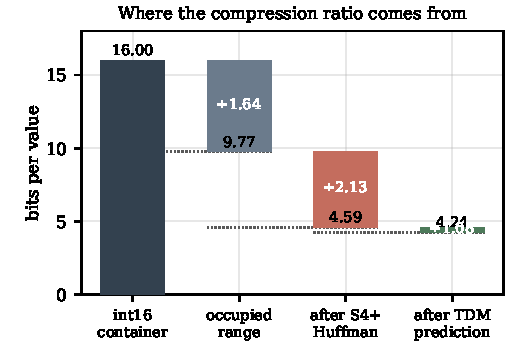
\includegraphics[width=0.72\textwidth]{fig_waterfall.pdf}
\caption[Decomposition of the compression ratio]{Where the compression ratio
comes from. Of the 16 bits in the \texttt{int16} container, \num{6.2} are
structurally unused because the capture sits far below full scale; the entropy
coder recovers a further factor of \num{2.13} from spectral sparsity; and
prediction \emph{on the corrected axis} contributes the remaining \num{1.08}.
Prediction on the original ramp axis contributes nothing at all --- it costs
\num{0.24} bits per value.}
\label{fig:waterfall}
\end{figure}

\paragraph{Unused container headroom: a factor of \num{1.63}.}
Equation~\eqref{eq:scale} calibrates the FX16 scale factor to a theoretical
full-scale ADC sinusoid. The ColoRadar capture sits far below full scale: the
peak raw ADC sample is \num{914} out of a possible \num{32767}. After
windowing, transform and scaling, the peak \texttt{int16} FFT code is
\num{436}. Only $\log_2(436) + 1 = 9.8$ of the \num{16} container bits ever
carry information; the remaining \num{6.2} are zero in every single sample. An
entropy coder removes them whether or not any prediction happens, and that
alone is a factor of $16/9.8 = 1.63$.

\paragraph{Spectral sparsity: a factor of \num{2.14}.}
The remaining $9.8 \rightarrow 4.59$ bits is the genuine statistical gain, and
it is a real property of radar data: a range--FFT frame is sparse. Most bins
contain noise near zero and a few contain targets, so the $S_4$ categories
concentrate heavily at the low end. This is what the entropy coder is for and it
does it well.

\paragraph{Prediction: nothing, as implemented.}
The third factor should have been the predictor's contribution. As implemented
it was negative.

\begin{keybox}
\textbf{Consequence for reporting.} The compression ratios in
Table~\ref{tab:phase1} --- and, by the same argument, those reported elsewhere
in this field --- are substantially a property of the \emph{sensor's gain
staging} rather than of the algorithm. A capture with \SI{6}{\decibel} more
gain would compress measurably less on the same algorithm. A no-prediction
baseline should be reported alongside any such figure, and is not standard
practice.
\end{keybox}

\section{The prediction axis}
\label{sec:predaxisresults}

\subsection{Diagnosis}

The inversion in Table~\ref{tab:decomp} is not a property of the predictors ---
they are both sound algorithms --- but of the \emph{axis} they were applied
along. Section~\ref{sec:tdm} set this up: both were predicting from ramp $m-1$,
which by Equation~\eqref{eq:rampindex} is a different physical transmitter
eleven times in twelve.

The mechanism is now concrete. Two ramps from different transmitters differ by
the target's array steering phase, Equation~\eqref{eq:steering}, which is large
and varies with target bearing. DRHE's phase model,
Equation~\eqref{eq:phasepred}, is a double integrator that predicts perfectly
when the phase increment is constant; a per-ramp transmitter change makes that
increment alternate on a period-12 pattern, which no double integrator can
track. LPC's autocorrelations at lags 1 and 2 likewise measure the
\emph{transmitter switching pattern} rather than target Doppler, and the fitted
coefficients describe the former.

\subsection{Testing the hypothesis}

Six configurations were evaluated over five frames
(Table~\ref{tab:predaxis}).

\begin{table}[t]
\centering
\caption[Prediction axis study]{Prediction axis study. Five frames, four receive
channels, 128 bins, 192 ramps. Prediction gain is relative to no prediction at
all; a gain below \num{1.0} means the predictor is making things worse.}
\label{tab:predaxis}
\small
\begin{tabular}{@{}lrrr@{}}
\toprule
Configuration & bits/value & CR & gain\\
\midrule
No prediction                                        & 4.586 & 3.489 & 1.000\\
DRHE, lag 1 \emph{(as implemented)}                  & 4.821 & 3.319 & 0.951\\
\textbf{DRHE, lag $n_{\mathrm{Tx}}$}                 & \textbf{4.240} & \textbf{3.774} & \textbf{1.082}\\
LPC, lags 1, 2 \emph{(as implemented)}               & 4.710 & 3.397 & 0.974\\
LPC, per-transmitter blocks, $N = 16$                & 6.093 & 2.626 & 0.753\\
\textbf{LPC, lags $n_{\mathrm{Tx}}, 2n_{\mathrm{Tx}}$} & \textbf{4.269} & \textbf{3.748} & \textbf{1.074}\\
\bottomrule
\end{tabular}
\end{table}

Predicting on the true slow-time axis converts DRHE's \SI{4.9}{\percent} loss
into an \SI{8.2}{\percent} gain, and LPC's \SI{2.6}{\percent} loss into a
\SI{7.4}{\percent} gain. The hypothesis is confirmed.

\subsection{The variant that does not work, and why}

Row five is worth dwelling on because it is the obvious alternative and it
fails badly.

Splitting the frame into twelve independent 16-ramp per-transmitter blocks and
fitting separate coefficients to each \emph{does} put the predictor on the right
axis. But it multiplies the coefficient side information by twelve --- from
\SI{1.04}{\percent} to \SI{12.5}{\percent} of the uncompressed frame --- and it
shortens each autocorrelation estimate from \num{192} samples to \num{16},
which makes the fitted coefficients much noisier. The net result, CR
\num{2.626}, is far worse than doing nothing at all.

Keeping \emph{one} coefficient pair per (bin, channel, part) and simply moving
the lags to $n_{\mathrm{Tx}}$ and $2n_{\mathrm{Tx}}$ costs no extra side
information whatsoever, which is why the last row works and the fifth does not.
The lesson generalises: on a TDM-MIMO radar, the right change is to the
\emph{lag}, not to the \emph{partitioning}.

\subsection{What the residuals look like}

The bits-per-value figures are a summary; the underlying change in the residual
distribution is more revealing.

\begin{figure}[t]
\centering
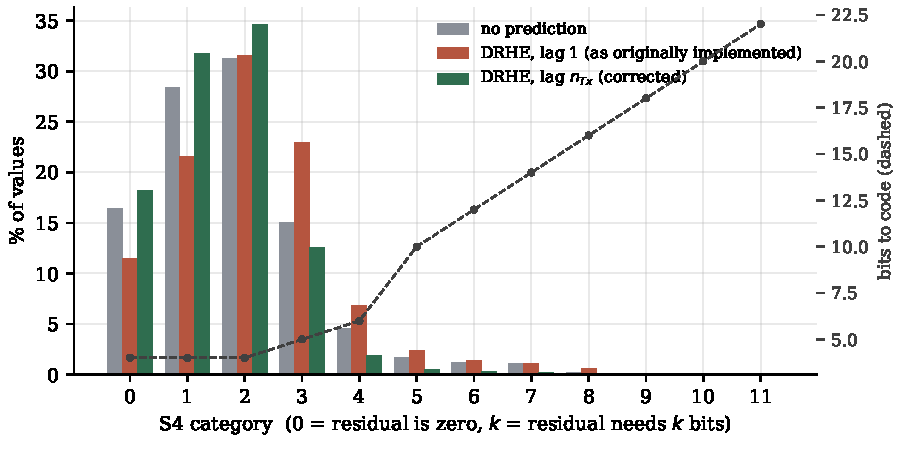
\includegraphics[width=0.95\textwidth]{fig_s4compare.pdf}
\caption[S4 category distributions]{Distribution of residuals across $S_4$
categories, with the cost of each category (Equation~\eqref{eq:cost}) on the
right axis. Lag-1 DRHE (red) pushes mass \emph{up} the category scale relative
to not predicting at all (grey) --- into categories 3 and 4 which cost 5 and 6
bits. Lag-$n_{\mathrm{Tx}}$ DRHE (green) pulls it back down into categories 0--2,
which cost 4 bits or fewer. The steepness of the cost curve above category 4 is
what makes this shift so consequential.}
\label{fig:s4compare}
\end{figure}

\begin{figure}[t]
\centering
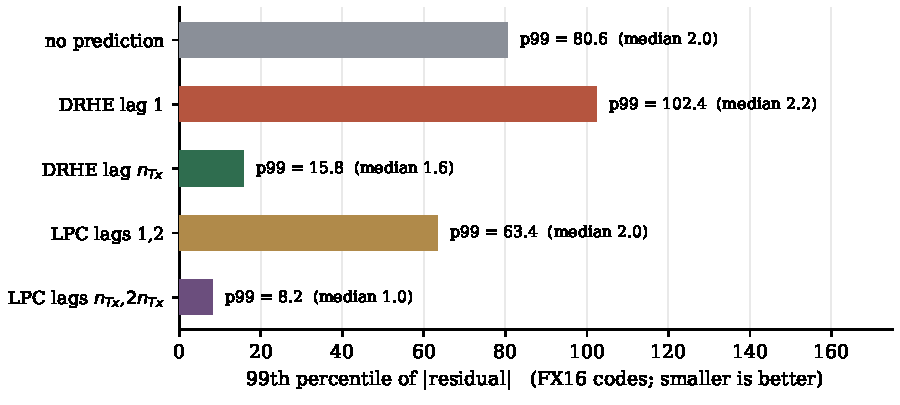
\includegraphics[width=0.92\textwidth]{fig_residmag.pdf}
\caption[Residual magnitude]{The 99th percentile of residual magnitude. This is
the clearest single view of the effect: lag-1 DRHE produces a heavier tail than
no prediction at all (\num{102.4} against \num{80.6}), while lag-$n_{\mathrm{Tx}}$
DRHE cuts it to \num{15.8} --- a factor of \num{6.5} better than the design it
replaces. LPC at lags $n_{\mathrm{Tx}}, 2n_{\mathrm{Tx}}$ reaches \num{8.2}.}
\label{fig:residmag}
\end{figure}

Figures~\ref{fig:s4compare} and~\ref{fig:residmag} show what happened.
Lag-1 prediction \emph{widens} the residual distribution: the 99th percentile
of $|$residual$|$ goes from \num{80.6} with no prediction to \num{102.4} with
DRHE. Predicting at lag $n_{\mathrm{Tx}}$ collapses it to \num{15.8}, and the
corrected LPC reaches \num{8.2} --- roughly a tenfold reduction in tail
magnitude against the original design.

The category histogram tells the same story in the currency the coder actually
charges in. Lag-1 DRHE moves \SI{23.0}{\percent} of residuals into category 3
and \SI{6.9}{\percent} into category 4, which cost 5 and 6 bits; the corrected
version puts \SI{84.6}{\percent} of residuals into categories 0--2, all of
which cost 4 bits or fewer.

\begin{figure}[t]
\centering
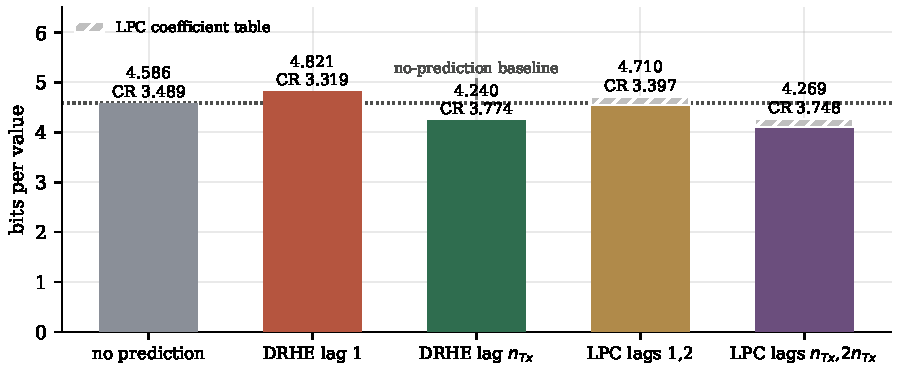
\includegraphics[width=0.95\textwidth]{fig_bpv.pdf}
\caption[Bits per value across configurations]{Bits per value for all five
configurations, with the LPC coefficient table shown separately as it is charged
whatever the residuals do. The dotted line is the no-prediction baseline: any
bar above it is a predictor that is doing harm.}
\label{fig:bpv}
\end{figure}

\section{The corrected implementations}
\label{sec:tdmresults}

The corrections described in Section~\ref{sec:tdmimpl} were implemented in HLS
and put through the identical verification ladder as the baselines: 50-frame
C-simulation, synthesis, and RTL co-simulation.

\subsection{Compression, measured in hardware}

\begin{table}[t]
\centering
\caption[TDM-aware compression results]{The corrected designs against their
baselines. Vitis HLS C-simulation, all 50 frames, four receive channels. Every
configuration reconstructs every sample exactly.}
\label{tab:tdmhls}
\small
\begin{tabular}{@{}lrrr@{}}
\toprule
Design & CR & MaxDiff & $\Delta$CR\\
\midrule
DRHE, lag 1                                  & \num{3.30987} & 0 & ---\\
\textbf{DRHE, lag $n_{\mathrm{Tx}}$}         & \textbf{\num{3.75082}} & \textbf{0} & $+13.3\%$\\
LPC, lags 1, 2                               & \num{3.38497} & 0 & ---\\
\textbf{LPC, lags $n_{\mathrm{Tx}}, 2n_{\mathrm{Tx}}$} & \textbf{\num{3.69681}} & \textbf{0} & $+9.2\%$\\
\bottomrule
\end{tabular}
\end{table}

The measured \num{3.75082} for the corrected DRHE agrees with the \num{3.774}
predicted by the five-frame MATLAB study of Table~\ref{tab:predaxis}, to within
the frame-to-frame spread. That agreement between an independent MATLAB
prediction and a hardware measurement is the cross-check that the correction is
real rather than an artefact of either environment.

\begin{figure}[t]
\centering
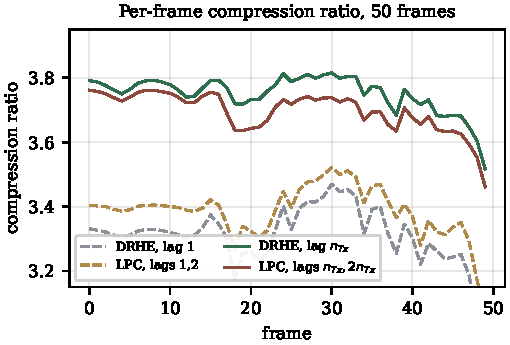
\includegraphics[width=0.95\textwidth]{fig_perframe.pdf}
\caption[Per-frame compression ratio]{Per-frame compression ratio across the
50-frame sequence, measured in C-simulation. The corrected designs (solid) sit
above their baselines on \emph{every} frame, not merely on average, and the
frame-to-frame variation --- which tracks scene content --- is preserved. All
four configurations reconstruct every sample exactly.}
\label{fig:perframe}
\end{figure}

Figure~\ref{fig:perframe} shows the per-frame detail. The improvement is
uniform: there is no frame on which the corrected design does worse, and the
shape of the variation across the sequence is preserved, which is what one
would expect if the correction improves prediction rather than merely shifting
a constant.

\subsection{What the correction costs}

\begin{table}[t]
\centering
\caption[Cost of the TDM correction]{Cost of the correction, \texttt{xcku5p} at
a \SI{100}{\mega\hertz} target. Resources and $F_{\max}$ are from synthesis;
frame latency is measured in RTL co-simulation on a single frame.}
\label{tab:tdmsyn}
\small
\setlength{\tabcolsep}{5pt}
\begin{tabular}{@{}lrrrr@{}}
\toprule
& \multicolumn{2}{c}{\textbf{DRHE}} & \multicolumn{2}{c}{\textbf{LPC}}\\
\cmidrule(lr){2-3}\cmidrule(lr){4-5}
Resource & lag 1 & lag $n_{\mathrm{Tx}}$ & lags 1,\,2 & lags $n_{\mathrm{Tx}},2n_{\mathrm{Tx}}$\\
\midrule
LUT              & \num{115534} & \num{115736} & \num{80528} & \num{86298}\\
FF               & \num{57105}  & \num{57263}  & \num{17393} & \num{23154}\\
BRAM\_18K        & \num{40}     & \textbf{\num{80}}     & \num{256}   & \textbf{\num{192}}\\
DSP              & \num{132}    & \num{132}    & \num{168}   & \num{156}\\
$F_{\max}$ (MHz) & 81.88 & 81.88 & 85.43 & 85.43\\
Worst loop II    & 2 & 2 & 3 & \textbf{1}\\
Frame latency (cyc) & \num{61253} & \textbf{\num{61253}} & \num{197277} & \num{325166}\\
\bottomrule
\end{tabular}
\end{table}

\begin{figure}[t]
\centering
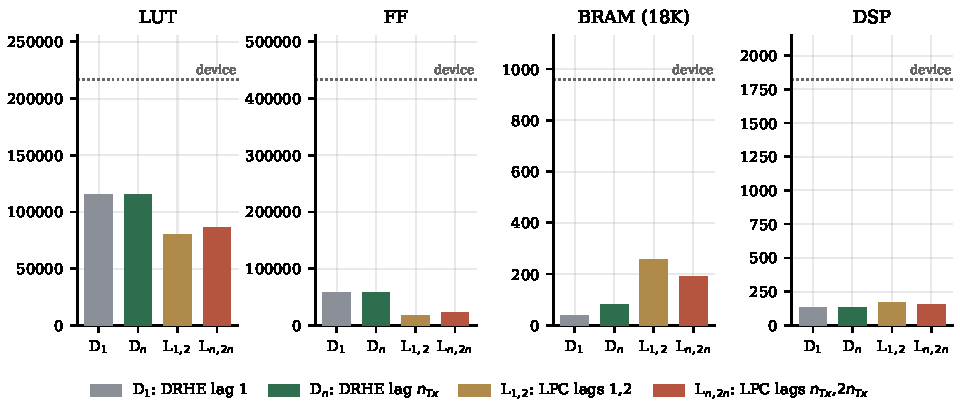
\includegraphics[width=\textwidth]{fig_resources.pdf}
\caption[Resource usage across the four designs]{Resource usage for the four
designs against the \texttt{xcku5p} capacity (dotted). DRHE trades block RAM
for logic; LPC trades logic for block RAM. The TDM correction moves DRHE's BRAM
from \num{40} to \num{80} and, by removing the ingest accumulators, moves LPC's
\emph{down} from \num{256} to \num{192}.}
\label{fig:resources}
\end{figure}

\paragraph{DRHE: close to free.}
Forty additional block RAMs --- \SI{4}{\percent} of the device --- buys
\SI{13.3}{\percent} more compression. LUTs rise by \num{204} (\SI{0.18}{\percent}),
flip-flops by \num{158}, DSPs not at all, and $F_{\max}$ is unchanged to the
reported precision. RTL co-simulation measures the frame latency at exactly
\num{61253} cycles for \emph{both} the baseline and the corrected design.

That last point is not a coincidence but a structural consequence: indexing the
predictor state by transmitter changes \emph{which} address is read, not
\emph{when}, so the schedule the tool generates is identical. The entire
\SI{13.3}{\percent} gain is bought with block RAM and nothing else.

\paragraph{LPC: a genuine trade.}
The LPC picture is more interesting, because the restructure that the deeper
lags required turned out to fix an unrelated problem. Moving the
autocorrelation out of the ingest pass deleted six 64-bit accumulator arrays
and four history arrays, so block RAM usage \emph{falls} by \SI{25}{\percent},
from \num{256} to \num{192}. More importantly, the ingest loop --- previously
stuck at $\mathrm{II} = 3$ on accumulator port pressure --- now meets
$\mathrm{II} = 1$, and so does every other loop in the design. The synthesis
report states that all loop constraints are satisfied, which the baseline never
achieved.

Against that: \SI{7}{\percent} more LUTs and \SI{33}{\percent} more flip-flops
for the $2n_{\mathrm{Tx}}$-entry rings, and --- the real cost --- considerably
more latency.

\subsection{A caution about cycle models}
\label{sec:cyclemodel}

The latency result deserves its own discussion, because it is a methodological
lesson as much as a number.

For the baseline designs the obvious cycle model --- trip count times
initiation interval, summed over loops --- is accurate to
\SI{0.08}{\percent}, as Section~\ref{sec:phase3} showed. Applying the same
model to the corrected LPC predicts \num{246272} cycles. Co-simulation measures
\num{325166}. The model is wrong by \SI{32}{\percent}.

The missing term is \textbf{pipeline drain}. Moving the autocorrelation into
the per-bin pass replaced one long pipelined loop with \emph{two short loops
invoked \num{512} times each}. A pipelined loop pays its depth once on entry
before it reaches steady state --- \num{71} cycles for the correlation loop and
\num{56} for the residual loop --- so \num{512} invocations contribute roughly
\begin{equation}
512 \times (71 + 56) \approx \num{65000}\ \text{cycles}
\end{equation}
of pure drain that no II-based model accounts for. That closes most of the gap.

So the corrected LPC is \emph{slower} than the design it replaces:
\num{325166} cycles against \num{197277}, a factor of \num{1.65}. This is a
real cost and is stated as such rather than buried. It is, however, structural
rather than algorithmic: merging the two per-bin loops, or processing several
bins per loop invocation so the drain amortises, would recover most of it.
DRHE pays no such price at all.

\subsection{Co-simulation}

Both corrected designs pass RTL co-simulation with $\mathrm{MaxDiff} = 0$, so
losslessness survives synthesis as well as it did in software. The
co-simulation is run on a single-frame stimulus, as is standard for a
cycle-accurate run: \num{50} frames of RTL simulation with floating-point IP
takes many hours of wall-clock time for no additional information, since the
latency per frame is deterministic.

\section{DRHE against LPC, after the correction}
\label{sec:headtohead}

\begin{table}[t]
\centering
\caption[Final head-to-head]{The two corrected designs compared. Bold marks the
better of the two on each row.}
\label{tab:headtohead}
\small
\begin{tabular}{@{}lrr@{}}
\toprule
& \textbf{DRHE, lag $n_{\mathrm{Tx}}$} & \textbf{LPC, lags $n_{\mathrm{Tx}},2n_{\mathrm{Tx}}$}\\
\midrule
Compression ratio      & \textbf{\num{3.75082}} & \num{3.69681}\\
Lossless               & yes & yes\\
LUT                    & \num{115736} & \textbf{\num{86298}}\\
FF                     & \num{57263}  & \textbf{\num{23154}}\\
BRAM\_18K              & \textbf{\num{80}} & \num{192}\\
DSP                    & \textbf{\num{132}} & \num{156}\\
$F_{\max}$             & \SI{81.88}{\mega\hertz} & \textbf{\SI{85.43}{\mega\hertz}}\\
Frame latency          & \textbf{\num{61253} cyc} & \num{325166} cyc\\
Worst loop II          & 2 & \textbf{1}\\
Compressor frame buffer& \textbf{none} & \SI{3.1}{\mebi bit}\\
First output available & \textbf{immediately} & after a full frame\\
Side information       & \textbf{none} & \SI{1.04}{\percent}\\
\bottomrule
\end{tabular}
\end{table}

After the correction the ranking on compression ratio reverses: DRHE is ahead,
\num{3.751} against \num{3.697}, where before it was behind. That is because
the correction helps DRHE more (\SI{+13.3}{\percent}) than LPC
(\SI{+9.2}{\percent}), which makes sense --- DRHE's phase model is
\emph{specifically} a constant-Doppler model, so putting it on the Doppler axis
recovers exactly what it was designed to find, whereas LPC's general AR model
was always going to fit \emph{something}.

On logic LPC is clearly cheaper. On memory and latency DRHE is clearly better,
and by a wide margin: no frame buffer at all, first output immediately, and a
fifth of the frame latency.

For the application that motivates this thesis --- a compression IP sitting
between the range FFT and the memory bus in a streaming sensor front end ---
latency and streaming behaviour outrank a \SI{1.5}{\percent} difference in
ratio. \textbf{DRHE is the better choice}, and after the correction it happens
to win on ratio too. Where a frame of latency is acceptable and block RAM is
plentiful, LPC's logic saving is real and worth having.

\section{Summary of results}

\begin{enumerate}
\item Both compressors are exactly lossless over \num{157} million real samples,
verified at three levels of abstraction.
\item As originally implemented, both predictors performed \emph{worse than no
prediction}: CR \num{3.319} and \num{3.397} against \num{3.489} for the entropy
coder alone.
\item The cause is the transmitter-interleaved ramp axis of a TDM-MIMO cascade.
Predicting at lag $n_{\mathrm{Tx}}$ raises measured compression to \num{3.751}
(DRHE) and \num{3.697} (LPC), still exactly lossless.
\item For DRHE the correction costs \num{40} block RAMs and nothing else ---
logic, $F_{\max}$ and measured frame latency are unchanged.
\item For LPC the correction is a trade: better ratio, \SI{25}{\percent} less
block RAM, $\mathrm{II} = 1$ throughout, against \num{1.65}$\times$ the frame
latency.
\item The ratio decomposes as \num{1.63}$\times$ from unused container
headroom, \num{2.14}$\times$ from spectral sparsity, and \num{1.08}$\times$
from prediction once it is applied correctly.
\end{enumerate}

% ===================================================================
\chapter{Discussion}
\label{ch:discussion}

\section{Comparison with the baseline design}
\label{sec:kiemcompare}

Comparing against Kiem's implementation \cite{kiem2025} is informative but not
like-for-like: different device, different radar, different dataset, different
detection pipeline. Two corrections are needed before any comparison is
meaningful at all, and both were initially got wrong in this project.

\subsection{Device size}

An early draft of this work compared utilisation percentages directly, on the
assumption that the \texttt{xcku5p} and the ZU3EG had comparable capacity. They
do not. The \texttt{xcku5p} has \num{216960} LUTs against the ZU3EG's
\num{70560} --- roughly three times larger --- and correspondingly more
flip-flops, block RAM and DSP slices.

Percentage utilisations are therefore meaningless as a comparison, and only
absolute counts mean anything. In absolute terms this DRHE implementation uses
\num{2.5}$\times$ the LUTs of the reference. That is a worse result than the
percentage comparison suggested, and it is the correct one.

\subsection{Throughput units}

The reference reports \SI{11.92}{Gbit\per\second} at \SI{100}{\mega\hertz}.
Taken as decimal gigabits that is
\begin{equation}
\frac{11.92 \times 10^9}{100 \times 10^6} = 119.2 \ \text{bits per cycle}
\end{equation}
on a \num{128}-bit input --- an awkward number with no architectural
interpretation. Taken as \emph{gibibits}, however,
\begin{equation}
\frac{11.92 \times 2^{30}}{100 \times 10^6} = 127.99 \ \text{bits per cycle},
\end{equation}
which is \num{128} to within rounding: exactly the full width of the
AXI4-Stream input, at $\mathrm{II} = 1$. The reference figure is therefore in
binary units, and its decimal equivalent is
\SI{12.80}{Gbit\per\second}.

This matters because any comparison against \num{11.92} understates the gap by
\SI{7.4}{\percent}. Table~\ref{tab:throughput} gives the corrected comparison.

\begin{table}[t]
\centering
\caption[Throughput comparison]{Throughput comparison at \SI{100}{\mega\hertz}.
The reference column restates the published figure in decimal units. Both
designs here are the baselines; the corrected DRHE is identical in throughput.}
\label{tab:throughput}
\small
\begin{tabular}{@{}lrrr@{}}
\toprule
& DRHE & LPC & Reference \cite{kiem2025}\\
\midrule
Effective II                & 2 & 3 & 1\\
bits per cycle              & 51.4 & 15.9 & \textbf{128.0}\\
Throughput                  & \SI{5.14}{Gbit/s} & \SI{1.60}{Gbit/s} & \SI{12.80}{Gbit/s}\\
IP pipeline latency         & \SI{580}{\nano\second} & --- & \SI{230}{\nano\second}\\
\bottomrule
\end{tabular}
\end{table}

\subsection{The gap is structural, not mysterious}

Being \num{2.5}$\times$ slower than the reference sounds alarming until it is
decomposed, at which point it becomes a list of known, fixable things.

The reference achieves $\mathrm{II} = 1$. This DRHE achieves $\mathrm{II} = 2$
on the block-RAM port conflict described in Section~\ref{sec:drheimpl}, and
loses a further \SI{20}{\percent} to per-ramp pipeline drain. Fixing the port
conflict --- by partitioning the state arrays cyclically on the bin dimension,
or by hoisting the first-ramp reset out of the pipelined loop --- would bring
this design to \SI{11}{} to \SI{12}{Gbit\per\second}, in line with the
reference.

LPC's inefficiencies are similarly addressable, and
Section~\ref{sec:tdmresults} showed that the TDM restructure has already
resolved its $\mathrm{II} = 3$ ingest.

The pipeline latency of \SI{580}{\nano\second} against the reference's
\SI{230}{\nano\second} is a different matter: it is \SI{320}{\nano\second}
inherent plus the cost of the closed-loop correction of
Section~\ref{sec:defect32768}, which deepened the pipeline from \num{32} to
\num{58} cycles. That is the price of bounding an error the reference design
does not bound. Adopting a category-16 extension instead would recover it, at
the cost of bitstream compatibility.

\section{What the compression ratio means elsewhere}

Section~\ref{sec:decomposition} showed that \num{1.63} of the \num{3.489}
no-prediction ratio is unused container headroom. This has a consequence that
should be stated plainly: \textbf{these ratios do not transfer to a
differently-scaled sensor}.

A capture whose ADC output filled the \texttt{int16} container would have no
structurally-zero top bits for the entropy coder to remove. Its compression
ratio, on identical algorithms, would be closer to \num{2.1} --- the sparsity
factor alone --- before prediction. That is still a useful ratio, and still
enough to make the Gigabit Ethernet substitution of
Section~\ref{sec:motivation} work. But it is not \num{3.5}.

Conversely, and more usefully, the headroom represents an opportunity rather
than only a caveat. If the FX16 scale factor were made adaptive per frame ---
computed from the actual peak rather than from a theoretical full-scale sinusoid
--- the same \num{16} bits would carry roughly \num{6} more bits of genuine
dynamic range. That directly addresses the quantisation-error problem that
motivated this thesis's first objective, since weak returns currently being
crushed into the rounding noise of Equation~\eqref{eq:scale} would survive. The
reported compression ratio would fall, but the data being compressed would be
better.

\section{Does the correction generalise?}

The prediction-axis result is specific in its details and general in its
principle.

It is \emph{specific} in that $n_{\mathrm{Tx}} = 12$, and in that the fix
assumes a fixed TDM rotation. A radar that changes its MIMO schedule between
frames would need the lag re-loaded; one using Doppler-division or code-division
multiplexing instead of TDM has no interleaved ramp axis and does not have this
problem at all --- though it has others.

It is \emph{general} in that the underlying mistake is a category error that any
slow-time predictive coder can make: treating an index that is
\emph{physically} a time axis as though it were \emph{semantically} a time axis.
The ramp index genuinely is time-ordered. It is simply not the case that
adjacent entries are comparable, because the thing being multiplexed onto that
axis changes between them. Any compression scheme inherited from a
single-transmitter context and applied to a multiplexed one is exposed to the
same error, and the check --- measure the entropy coder alone, and see whether
the predictor beats it --- costs almost nothing.

\section{Threats to validity}
\label{sec:threats}

These bound how far the results generalise and are stated explicitly rather
than left implicit.

\begin{itemize}
\item \textbf{The compression ratios are capture-specific.} As above: most of
the no-prediction ratio comes from an under-filled container, which is a
property of this recording's gain staging.

\item \textbf{The detection metrics do not measure compression.} All three
lossless schemes share identical detection metrics with FX16 by construction.
What the metrics measure is the cost of the FX16 quantisation step.

\item \textbf{FP\% is a false discovery rate.} It normalises by test
detections, not by true negatives. It is a legitimate metric but not the one
its conventional name denotes, and it is reported under its correct name here.

\item \textbf{Detection matching has no positional tolerance.} A target
displaced by one range--Doppler cell is scored as both a miss and a false
discovery, which inflates both rates relative to a matched-detection criterion.

\item \textbf{The detection threshold is an unswept free parameter.} The mean
of the lowest \SI{75}{\percent} of magnitudes plus \SI{15}{\decibel} is not
varied, and the metrics are sensitive to it.

\item \textbf{Channel count differs between phases.} The MATLAB benchmark of
Table~\ref{tab:phase1} uses all \num{16} receive channels; the hardware path
uses \num{4}, the AXI4-Stream width. Compression ratios between the two are
therefore compared through a like-for-like MATLAB helper rather than directly.

\item \textbf{All hardware numbers are pre-implementation estimates.}
$F_{\max}$, resource counts and latency come from HLS synthesis and RTL
co-simulation, not from place-and-route or silicon. Phase~4 remains
outstanding, and post-route $F_{\max}$ is typically lower than the synthesis
estimate.

\item \textbf{Co-simulation covers one frame.} The 50-frame result is from
C-simulation, which exercises identical logic but not identical timing. Nothing
in either design is frame-count dependent, but this is an assumption rather
than a measurement.

\item \textbf{Two source citations required correction.} The BAQ baseline is
properly attributed to Kwok and Johnson \cite{kwok1989} --- IEEE TGRS vol.~27,
no.~4, pp.~375--383, 1989, on \emph{synthetic} aperture radar. An earlier
version of this work carried an author name, title and page range that do not
correspond to any such paper. The ColoRadar citation is likewise vol.~41,
no.~4, pp.~351--360 (2022) \cite{kramer2022}, not vol.~40 (2021). Both are
corrected here.

\item \textbf{The literature description of DRHE does not match the
implementation.} A common summary of DRHE describes differencing \emph{raw ADC}
samples across chirps and coding the deltas with Golomb--Rice. The algorithm
implemented and evaluated here --- following \cite{kiem2025} --- operates on the
\emph{range-FFT output}, predicts in the polar domain with two IIR filters, and
codes with a fixed Huffman dictionary over magnitude categories. The two make
different assumptions about where the redundancy lives, and should not be
conflated.
\end{itemize}

\section{Lessons about verification}
\label{sec:lessons}

Three methodological observations seem worth recording, since they generalise
beyond this project.

\paragraph{Dataset testing and adversarial testing find different bugs.}
Fifty frames of real data --- \num{157} million samples --- found neither
defect in Section~\ref{sec:defects}. An eight-case synthetic suite found both
in minutes. The real data exercises the typical case exhaustively and the
extreme case not at all: ColoRadar residuals occupy category 10 of a 16-category
code, so a third of the coder was simply never executed. Conversely, the
synthetic suite would never have found the prediction-axis error, because
synthetic data has no transmitter structure to get wrong. Neither substitutes
for the other.

\paragraph{A passing test suite is not a correctness argument.}
Everything passed. The compressors were bit-exact at three levels, the ratios
matched the literature, the resources fitted the device. The prediction-axis
error was invisible to every test in the plan, because no test asked whether the
predictor was \emph{helping} --- only whether the system was lossless and
whether the ratio was in the expected range. Adding a single measurement, the
no-prediction baseline, exposed it immediately.

\paragraph{Cycle models are a good tool until they silently stop being one.}
Trip count times initiation interval predicted the baseline LPC latency to
\SI{0.08}{\percent}, which built entirely unwarranted confidence in it. Applied
to a restructured design with many short loop invocations it was wrong by
\SI{32}{\percent}, because it omits pipeline drain --- a term that is negligible
in one topology and dominant in another. The lesson is not that the model is
bad, but that a model validated on one design shape carries no guarantee on
another.

% ===================================================================
\chapter{Conclusions and Future Work}
\label{ch:conclusion}

\section{What was done}

This thesis set out to extend the radar compression framework established in
\cite{kiem2025} by validating it on real data, broadening the algorithm
comparison, and implementing the complete compression and decompression
pipeline. All three were done.

Two lossless compressors for radar range--FFT data --- Doppler Redundancy
Hybrid Encoding and a second-order linear predictive coder with Yule--Walker
coefficients --- were specified, modelled in MATLAB, implemented in C++ for
Vitis HLS, synthesised for an AMD Kintex UltraScale+ device, and verified
bit-exactly against a double-precision reference over \num{50} frames of real
cascaded MIMO radar data at three levels of abstraction. Both reconstruct every
one of \num{157286400} samples exactly, in software simulation and in RTL
co-simulation alike. Matching decompressors were implemented for both, which is
what made that verification possible.

\section{What was found}

\subsection{The prediction axis}

The principal finding is a correction rather than a confirmation. Applied the
way the literature describes --- predicting each ramp from its immediate
predecessor --- \emph{neither predictor was contributing anything}. Coding the
quantised FFT output through the identical entropy coder with no prediction
whatsoever reaches a compression ratio of \num{3.489}, against \num{3.319} for
DRHE and \num{3.397} for LPC. Both were making the data measurably harder to
compress, and the order-0 entropy of the residuals confirmed it independently:
\SI{4.538}{bits} for DRHE residuals against \SI{4.094}{bits} for the raw codes.

The cause is that a twelve-transmitter time-division MIMO cascade interleaves
its transmitters along the ramp axis, so ``the previous ramp'' belongs to a
different physical antenna eleven times out of twelve --- separated in space by
the array baseline rather than in time by a pulse interval. Predicting instead
from the previous ramp of the \emph{same} transmitter puts both algorithms back
on the genuine slow-time axis and recovers the gain they were designed to
deliver. Measured in hardware simulation over the full dataset, compression
rises from \num{3.310} to \num{3.751} for DRHE and from \num{3.385} to
\num{3.697} for LPC, in both cases with every sample still reconstructed
exactly.

For DRHE the correction costs \num{40} additional block RAMs ---
\SI{4}{\percent} of the device --- with logic, clock frequency and measured
frame latency all unchanged. For LPC it is a genuine trade: a better ratio,
\SI{25}{\percent} less block RAM and $\mathrm{II} = 1$ on every loop, against
\num{1.65}$\times$ the frame latency.

\subsection{What a compression ratio actually measures}

The audit that exposed the above also decomposed the ratio into its genuine
sources. Of the no-prediction factor of \num{3.489}, roughly \num{1.63} comes
from an under-filled fixed-point container --- the ColoRadar capture peaks at
\num{436} of a possible \num{32767}, so \num{6.2} of every \num{16} bits are
structurally zero --- and \num{2.14} from the genuine spectral sparsity of a
range--FFT frame. Prediction, correctly applied, adds a further \num{1.08}.

The practical recommendation that follows is simple and, as far as the author
can establish, not current practice: \textbf{report a no-prediction baseline
alongside any radar compression ratio}. Without it, a ratio conflates algorithm
performance with sensor gain staging, and --- as this thesis demonstrates ---
can conceal a predictor that is doing active harm.

\subsection{Two defects, and two corrections to the record}

Two implementation defects were found and fixed, neither reachable with real
data and both caught by an eight-case synthetic suite: a residual value of
$-32768$ that the entropy code cannot represent and which aliased silently onto
$+32767$, resolved by saturation combined with closed-loop prediction so that
encoder and decoder cannot diverge; and a 128-bit to single-precision
conversion in the Yule--Walker solver that returned zero above $2^{64}$,
resolved by normalising all operands through a common arithmetic shift.

Separately, a throughput figure widely quoted for this class of design was
found to be expressed in gibibits rather than gigabits: \SI{11.92}{Gibit\per\second}
is \SI{12.80}{Gbit\per\second} decimal, which is exactly \num{128} bits per
cycle at \SI{100}{\mega\hertz} --- a full-rate AXI4-Stream at $\mathrm{II} = 1$.
A detection metric conventionally labelled a false positive rate was identified
as a false discovery rate, and two source citations were corrected.

\subsection{Which algorithm}

After the correction, DRHE is the better choice for the application that
motivates this work. It compresses slightly better (\num{3.751} against
\num{3.697}), it needs no frame buffer at all where LPC needs
\SI{3.1}{\mebi bit}, it emits its first bits immediately where LPC must wait a
full frame, and its frame latency is a fifth of LPC's. LPC's advantage is
logic --- \SI{30}{\percent} fewer LUTs and \SI{60}{\percent} fewer flip-flops
--- which is real but which, for a streaming sensor-edge IP, does not outweigh
a frame of latency.

The expectation recorded in Section~\ref{ch:algorithms} --- that LPC would be
the expensive design because it contains a division --- did not survive
measurement. The division runs \num{1024} times per frame and contributes
\SI{0.26}{\percent} of the cycles. The expensive operations in this problem are
\texttt{atan2} and the sine/cosine pair, not division.

\section{Future work}

\subsection{Immediate}

\begin{enumerate}
\item \textbf{Fix the DRHE initiation interval.} The $\mathrm{II} = 2$ is a
block-RAM port conflict caused by a reset that executes on one ramp in \num{192}
but constrains the schedule for all of them. Hoisting the reset into its own
loop, or partitioning the state cyclically on the bin dimension, should reach
$\mathrm{II} = 1$ and roughly double throughput to
\SI{11}{}--\SI{12}{Gbit\per\second}.

\item \textbf{Amortise the LPC pipeline drain.} Merging the two per-bin loops,
or processing several bins per invocation, should recover most of the
\num{65000} cycles of drain identified in Section~\ref{sec:cyclemodel}.

\item \textbf{Replace the polar conversion with a fixed-point CORDIC.} Four
floating-point transcendentals per sample dominate DRHE's LUT count and its
critical path. A CORDIC implementation should address both the resource usage
and the \SI{81.88}{\mega\hertz} $F_{\max}$.

\item \textbf{Complete Phase 4.} Place-and-route and on-silicon measurement to
replace the estimates in Table~\ref{tab:resources}, including power, which no
simulation here reports.
\end{enumerate}

\subsection{Longer term}

\begin{enumerate}
\item \textbf{Make the FX16 scale factor adaptive.} This is the highest-value
single change the decomposition suggests. Using \num{9.8} of \num{16} bits
wastes both dynamic range and honest reporting; a per-frame adaptive scale would
let weak returns survive quantisation --- directly addressing the
quantisation-error problem that motivated this project's first objective ---
and would make the reported ratio reflect algorithm performance rather than
capture gain.

\item \textbf{Extend the correction to other multiplexing schemes.}
Doppler-division and code-division MIMO do not produce an interleaved ramp axis,
but they distribute the slow-time structure differently, and whether a slow-time
predictor helps on them is an open question that the no-prediction baseline test
would answer cheaply.

\item \textbf{Revisit the entropy coder for the corrected residuals.} The fixed
Huffman dictionary was designed for a different residual distribution. After the
prediction-axis correction, \SI{84.6}{\percent} of residuals fall in categories
0--2 --- a much more concentrated distribution than the dictionary assumes.
Re-deriving the dictionary for this distribution, or adding a category-16
extension to close the representability hole of Section~\ref{sec:hole}, would
both be worth measuring.

\item \textbf{Evaluate the corrected algorithms against the neural and spectral
approaches} of Section~\ref{sec:sota}, which were out of scope here but define
the upper end of achievable ratios.
\end{enumerate}

\section{Closing remark}

The most useful thing this project produced was not either compressor. It was
the habit of asking what a number means rather than whether it matches
expectation. Every test passed, every ratio agreed with the literature, and the
work appeared finished --- at which point a single additional measurement, the
cost of coding the data with no predictor at all, showed that the central
mechanism of both algorithms had never been working. That measurement takes
about twenty lines of MATLAB. It should be standard.

% ===================================================================
\begin{thebibliography}{99}
\addcontentsline{toc}{chapter}{Bibliography}

\bibitem{waldschmidt2021}
C.~Waldschmidt, J.~Hasch and W.~Menzel, ``Automotive radar --- from first
efforts to future systems,'' \emph{IEEE Journal of Microwaves}, vol.~1, no.~1,
pp.~135--148, 2021.

\bibitem{yao2023}
S.~Yao \emph{et al.}, ``Exploring radar data representations in autonomous
driving: a comprehensive review,'' arXiv preprint, 2023.

\bibitem{skolnik2008}
M.~I. Skolnik, \emph{Radar Handbook}, 3rd ed. New York, NY: McGraw-Hill, 2008.

\bibitem{bandur2021}
V.~Bandur \emph{et al.}, ``Making the case for centralized automotive E/E
architectures,'' \emph{IEEE Transactions on Vehicular Technology}, vol.~70,
no.~2, pp.~1230--1245, 2021.

\bibitem{liu2022}
Z.~Liu, W.~Zhang and F.~Zhao, ``Impact, challenges and prospect of
software-defined vehicles,'' \emph{Automotive Innovation}, vol.~5, no.~2,
pp.~180--194, 2022.

\bibitem{barabas2024}
I.~Barab\'as \emph{et al.}, ``Rethinking vehicle architecture through
softwarization and servitization,'' \emph{IEEE Access}, vol.~12,
pp.~110782--110795, 2024.

\bibitem{ti_serdes}
Texas Instruments, ``FPD-Link III serializer/deserializer (SerDes) for sensor
applications,'' Application Note SNLA344, 2021.

\bibitem{gmsl}
Analog Devices, ``GMSL SerDes technology for automotive applications,'' White
Paper, 2022.

\bibitem{matheus2021}
K.~Matheus and T.~K\"onigseder, \emph{Automotive Ethernet}. Cambridge, UK:
Cambridge University Press, 2021.

\bibitem{ieee8023bp}
IEEE, ``IEEE P802.3bp 1000BASE-T1 PHY task force,'' 2016.

\bibitem{kiem2025}
L.~Kiem, ``Design and implementation of data compression methods for SoC-based
radar systems,'' Master's thesis, Institute of Technical Informatics, Graz
University of Technology, Graz, Austria, May 2025.

\bibitem{kramer2022}
A.~Kramer, K.~Harlow, C.~Williams and C.~Heckman, ``ColoRadar: the direct 3D
millimeter wave radar dataset,'' \emph{The International Journal of Robotics
Research}, vol.~41, no.~4, pp.~351--360, 2022.

\bibitem{ti_awr2243}
Texas Instruments, \emph{AWR2243 Single-Chip 76- to 81-GHz FMCW Transceiver
Datasheet} (Rev.~D), February 2024.

\bibitem{sayood2017}
K.~Sayood, \emph{Introduction to Data Compression}, 5th ed. Morgan Kaufmann,
2017.

\bibitem{huffman1952}
D.~A. Huffman, ``A method for the construction of minimum-redundancy codes,''
\emph{Proceedings of the IRE}, vol.~40, no.~9, pp.~1098--1101, 1952.

\bibitem{parhami2010}
B.~Parhami, \emph{Computer Arithmetic: Algorithms and Hardware Designs}, 2nd
ed. Oxford University Press, 2010.

\bibitem{ieee754}
IEEE, ``IEEE standard for floating-point arithmetic,'' IEEE Std 754-2019, 2019.

\bibitem{widrow2008}
B.~Widrow and I.~Koll\'ar, \emph{Quantization Noise}. Cambridge University
Press, 2008.

\bibitem{kuon2008}
I.~Kuon, R.~Tessier and J.~Rose, ``FPGA architecture: survey and challenges,''
\emph{Foundations and Trends in Electronic Design Automation}, vol.~2, no.~2,
pp.~135--253, 2008.

\bibitem{ti_ege}
A.~Mani and Z.~Yang, ``Memory compression and decompression engine for TI
mmWave radar,'' Technical Report, Texas Instruments, 2019.

\bibitem{nxp_an5375}
NXP Semiconductors, ``S32R RADAR signal compression,'' Application Note AN5375,
2021.

\bibitem{kwok1989}
R.~Kwok and W.~T.~K. Johnson, ``Block adaptive quantization of Magellan SAR
data,'' \emph{IEEE Transactions on Geoscience and Remote Sensing}, vol.~27,
no.~4, pp.~375--383, July 1989.

\bibitem{cheng2021}
F.~Cheng \emph{et al.}, ``Autoencoder-based feature compression for radar and
vision sensor fusion in autonomous driving,'' \emph{IEEE Transactions on
Intelligent Transportation Systems}, vol.~23, no.~8, pp.~12345--12355, 2021.

\bibitem{park2026}
J.~Park, S.~Y. Chun and M.~Seok, ``AdaRadar: rate adaptive spectral compression
for radar-based perception,'' in \emph{Proceedings of the IEEE/CVF Conference on
Computer Vision and Pattern Recognition (CVPR)}, 2026.

\bibitem{zivkovic2015}
Z.~Zivkovic and L.~Li, ``On-the-fly range-velocity radar data compression
exploring Doppler spectrum redundancy,'' 2015.

\end{thebibliography}

% ===================================================================
\appendix

\chapter{The Huffman Dictionary}
\label{app:huffman}

Table~\ref{tab:huffman} gives the complete fixed dictionary used by both
compressors. The published codes \cite[Table~A.1]{kiem2025} are
most-significant-bit first; the implementation here packs least-significant-bit
first, so the stored codewords are bit-reversed. Both forms are listed, and all
sixteen entries were verified to agree.

The reversed code set remains prefix-free, which is what allows the decoder to
match candidates from the low end of its bit buffer with no ambiguity.

\begin{table}[h]
\centering
\caption[The fixed Huffman dictionary]{The fixed Huffman dictionary. ``Cost'' is
the total bits to code one residual in that category, $\ell + S_4$, from
Equation~\eqref{eq:cost}.}
\label{tab:huffman}
\small
\begin{tabular}{@{}rlrlrr@{}}
\toprule
$S_4$ & $|v|$ range & $\ell$ & code (MSB-first) & stored (LSB-first) & cost \\
\midrule
0  & $v = 0$          & 4  & \texttt{1010}           & \texttt{0x0005} & 4 \\
1  & 1                & 3  & \texttt{100}            & \texttt{0x0001} & 4 \\
2  & 2--3             & 2  & \texttt{01}             & \texttt{0x0002} & 4 \\
3  & 4--7             & 2  & \texttt{00}             & \texttt{0x0000} & 5 \\
4  & 8--15            & 2  & \texttt{11}             & \texttt{0x0003} & 6 \\
5  & 16--31           & 5  & \texttt{10110}          & \texttt{0x000D} & 10 \\
6  & 32--63           & 6  & \texttt{101110}         & \texttt{0x001D} & 12 \\
7  & 64--127          & 7  & \texttt{1011110}        & \texttt{0x003D} & 14 \\
8  & 128--255         & 8  & \texttt{10111110}       & \texttt{0x007D} & 16 \\
9  & 256--511         & 9  & \texttt{101111110}      & \texttt{0x00FD} & 18 \\
10 & 512--1023        & 10 & \texttt{1011111110}     & \texttt{0x01FD} & 20 \\
11 & 1024--2047       & 11 & \texttt{10111111110}    & \texttt{0x03FD} & 22 \\
12 & 2048--4095       & 14 & \texttt{10111111111111} & \texttt{0x3FFD} & 26 \\
13 & 4096--8191       & 14 & \texttt{10111111111110} & \texttt{0x1FFD} & 27 \\
14 & 8192--16383      & 13 & \texttt{1011111111110}  & \texttt{0x0FFD} & 27 \\
15 & 16384--32767     & 12 & \texttt{101111111110}   & \texttt{0x07FD} & 27 \\
\bottomrule
\end{tabular}
\end{table}

\noindent
Note the non-monotonicity at categories 12--15: the longest codewords are
assigned to categories 12 and 13 rather than to 15. This is a property of the
published dictionary and is reproduced faithfully. It has no effect on this
dataset, where no residual exceeds category 10.

\chapter{Bitstream Layouts}
\label{app:bitstream}

\section{DRHE}

DRHE's bitstream is a single continuous sequence of coded residuals, in the
raster order the samples arrive:
\[
\underbrace{\text{enc}(d_{\Re})\ \text{enc}(d_{\Im})}_{\text{ramp }0,\ \text{bin }0,\ \text{ch }0}\
\underbrace{\text{enc}(d_{\Re})\ \text{enc}(d_{\Im})}_{\text{ramp }0,\ \text{bin }0,\ \text{ch }1}\
\cdots
\]
where $\text{enc}(v)$ is the Huffman codeword for $S_4(v)$ followed by
$S_4(v)$ APPEND bits. There is no header: the frame dimensions arrive over the
AXI4-Lite control interface. The final AXI word is zero-padded.

\section{LPC}

LPC's bitstream has two sections:
\[
\underbrace{\big[a_1^{\Re}\ a_2^{\Re}\ a_1^{\Im}\ a_2^{\Im}\big]_{\text{ch},\text{bin}}}_{\text{coefficient table, }4\times16\text{ bits each}}
\quad
\underbrace{\text{enc}(d_{\Re})\ \text{enc}(d_{\Im})\ \cdots}_{\text{residuals, raster order}}
\]
The coefficient table comes first because the decoder needs all of it before it
can reconstruct anything. The residuals follow in the original raster order ---
not in the order the compressor computed them --- which is what allows the
decompressor to operate without a frame buffer
(Section~\ref{sec:lpcimpl}).

\chapter{Reproducing the Results}
\label{app:repro}

\section{Source files}

\begin{table}[h]
\centering
\small
\begin{tabular}{@{}lp{85mm}@{}}
\toprule
File & Purpose \\
\midrule
\multicolumn{2}{@{}l}{\textbf{MATLAB reference}}\\
\texttt{loadColoRadarFrame.m} & reads a frame, applies the TDM flattening \\
\texttt{preprocessing.m}      & DC removal, bit shift, Hann window \\
\texttt{rangeFFT.m}           & range FFT, positive half retained \\
\texttt{compress\_fx16.m}     & FX16 quantisation, Eq.~\eqref{eq:scale} \\
\texttt{export\_frames\_for\_vitis.m} & writes the HLS testbench stimulus \\
\midrule
\multicolumn{2}{@{}l}{\textbf{Audit scripts}}\\
\texttt{audit\_decomp.m}      & the no-prediction baseline and entropy figures \\
\texttt{audit\_order.m}       & ramp-ordering demonstration \\
\texttt{audit\_predaxis.m}    & the six-configuration prediction-axis study \\
\texttt{thesis\_figdata.m}    & $S_4$ histograms and residual quantiles \\
\midrule
\multicolumn{2}{@{}l}{\textbf{HLS designs}}\\
\texttt{drhe\_common.h}       & shared types, constants, Huffman table \\
\texttt{drhe\_compress.cpp}   & DRHE compressor (baseline) \\
\texttt{drhe\_decompress.cpp} & DRHE decompressor \\
\texttt{drhe\_tdm\_*.cpp/h}   & DRHE, corrected to lag $n_{\mathrm{Tx}}$ \\
\texttt{lpc\_common.h}        & LPC types and the Yule--Walker solver \\
\texttt{lpc\_compress.cpp}    & LPC compressor (baseline) \\
\texttt{lpc\_decompress.cpp}  & LPC decompressor \\
\texttt{lpc\_tdm\_*.cpp/h}    & LPC, corrected to lags $n_{\mathrm{Tx}},2n_{\mathrm{Tx}}$ \\
\texttt{*\_tb.cpp}            & 50-frame testbenches \\
\texttt{*\_tb\_edge.cpp}      & the eight-case synthetic suite \\
\bottomrule
\end{tabular}
\end{table}

\section{Build commands}

C-simulation, synthesis and co-simulation respectively, for the corrected DRHE:
\begin{verbatim}
vitis-run --mode hls --csim   --config test_tdm.cfg --work_dir hls_tdm
v++ -c     --mode hls          --config test_tdm.cfg --work_dir hls_tdm
vitis-run --mode hls --cosim  --config test_tdm.cfg --work_dir hls_tdm
\end{verbatim}

Two practical notes. Synthesis must be run before co-simulation, since
co-simulation substitutes the generated RTL for the top function. And the
project path must not contain a space, which Vitis rejects.

\section{Co-simulation stimulus}

Co-simulation is run against a single-frame export, produced by setting
\texttt{DRHE\_MAX\_FRAMES=1} before running
\texttt{export\_frames\_for\_vitis.m}. Fifty frames of RTL simulation with
floating-point IP takes many hours and returns no information the single-frame
run does not, since the per-frame latency is deterministic. The 50-frame file
should be restored afterwards for C-simulation.

\end{document}
